\documentclass[modern]{aastex62}

\newcommand{\R}{{\normalfont\textsf{R}}{}}

\usepackage{listings}
\lstset{
  basicstyle=\footnotesize,
  numbers=left,
  stepnumber=1,
  breaklines=true
}

\begin{document}


\title{Bayesian nonparametric star formation histories: models, methods, and a case study}
\author{Michael Peck}
\noaffiliation
\email{mlpeck54@gmail.com}
	
\DeclareGraphicsExtensions{.jpg, .pdf, .png, .eps}
	
\defcitealias{2010MNRAS.405..783M}{M10}
\defcitealias{2003MNRAS.344.1000B}{BC03}
\defcitealias{2012A&A...543A.132C}{C12}
\defcitealias{2013MNRAS.432..359T}{T13}

\begin{abstract}
Astronomers have produced models of the spectral energy distributions of galaxies for almost as long as their extragalactic nature has been recognized. Stellar population synthesis has been a quantitative discipline since at least the early 1970's thanks to advances in stellar evolution theory and computational tools that became available at that time. Since then a large number of tools have been developed for SED modeling, including several that have been made publicly available. To my knowledge however there has not to date been a successful fully Bayesian implementation of a tool for SED fitting with a nonparametric model of star formation histories. I show that the variant of Hamiltonian Monte Carlo implemented in the modeling language Stan is (perhaps uniquely) capable of converging to a stationary posterior distribution in a tractable number of iterations with dozens or even hundreds of input template spectra. I demonstrate its performance on a small number of mock data sets and on a sample of spiral galaxies in the first public data release of SDSS-IV MaNGA.
\end{abstract}


\section{INTRODUCTION}
\label{sec:intro}

The spectral energy distributions (SEDs) of galaxies contain archaeological records of their star formation histories and present physical properties. This simple truism has been understood for a very long time \citep{1935hcoc404} and a vast literature is devoted to extracting information from SED's. For recent reviews of the subject see \citet{2013ARA&A..51..393C, 2011Ap&SS.331....1W, 2012IAUS..284....2L}. Earlier reviews include \citet{2000eaa..bookE2870W, 1996ASPC...98....3O, 1980FCPh....5..287T}. In this paper I focus on full SED fitting, that is the observational data are colors or relative or absolute monochromatic fluxes, and I specifically concentrate on spectroscopic data. The alternative approach of treating absorption line indexes as the observable data \citep{2012MNRAS.421.1678Z, 1994ApJS...95..107W, 1994ApJS...94..687W} will not be considered here except in passing.

SED modeling was first made fully quantitative by \citet{1972A&A....20..361F} who formulated the problem as a quadratic program, which is a linearly constrained optimization model with quadratic objective function. Nearly 50 years later there is still no standardized approach to the task, and papers continue to appear regularly offering new takes on the subject. Several computer codes are publicly available however and at least two of these -- \texttt{ppxf} \citep{2004PASP..116..138C, 2017MNRAS.466..798C} and \texttt{STARLIGHT} \citep{2005MNRAS.358..363C} -- are close to becoming standard tools thanks to being incorporated into the data processing pipelines of large IFU based spectroscopic surveys \citep{2016AJ....152...83L, fernandes_et_al._2014}. A non-comprehensive list of others include PEGASE \citep{1997A&A...326..950F, 1999astro.ph.12179F}, GALEXEV \citep{2003MNRAS.344.1000B}, STECKMAP \citep{2006MNRAS.365...46O, 2006MNRAS.365...74O, 2011arXiv1108.4631O}, ULySS \citep{2009A&A...501.1269K}, FSPS \citep{2009ApJ...699..486C, 2010ApJ...712..833C}, CIGALEMC \citep{2011ApJ...740...22S}, GalMC \citep{2011ApJ...737...47A}, and StarPy \citep{2016ascl.soft09002S, 2015MNRAS.450..435S}. In addition a great many codes have been developed internally but never publicly released, some of which have been used to create large catalogs of stellar population properties \citep{2004astro.ph..6220B, 2007MNRAS.381.1252T, 2009ApJS..185....1T}.

There are two common approaches to model the star formation histories (SFH) of galaxies, which is an important (but not only) aspect of SED modeling and the main topic of interest in this paper. One is to assume a functional form for the time evolution of the star formation rate. An exponentially decaying (or increasing) star formation rate (SFR) is commonly adopted, but other forms including top hat functions, delta functions (i.e. all star formation occcuring in a single burst), and ``delayed $\tau$'' models ($SFR \propto t/\tau \mathrm{e}^{-t/\tau}$) have been used. All of these functions are unimodal and as such cannot model more complex multimodal star formation histories such as late time starbursts, which if considered at all are usually added as delta functions. They also have known biases when model assumptions aren't met \citep{2009ApJS..184..100L}. 

The other common approach is what \citet{2013ARA&A..51..393C} calls ``non-parametric'' star formation histories where the model inputs are typically a basis set of spectra of coeval populations of differing ages. The star formation history is then inferred from the relative contributions of each population. \citet{2013ARA&A..51..393C} considers this to be the most promising way to obtain detailed and unbiased estimates of star formation histories and in fact this approach is used by both \texttt{ppxf} and \texttt{STARLIGHT}, which judging by citation counts are probably the most popular modeling codes.

There are also two commonly adopted approaches to inference among programs that attempt to fit SEDs (some of the mentioned programs generate model predictions but don't attempt to fit data): these can be broadly characterized as optimization and Bayesian methods. Optimization methods seek the maximum (possibly penalized) likelihood solution for model parameters. Bayesian methods attempt to explore the posterior distribution of model parameters using Markov Chain Monte Carlo (MCMC) techniques. An interesting bimodality exists in the codes mentioned above (and other unreleased ones): all of the programs that use MCMC methods adopt a parametric form for star formation histories, while all of the programs that explore non-parametric star formation histories use maximum likelihood methods (occasionally implemented with heuristic algorithms that, with luck, might approximate ML solutions). The only partial exception I could find in the literature was \citet{2001MNRAS.325...60C}, who used an MCMC algorithm to explore the posterior of contributions from a basis set of 12 star clusters of varying ages and metallicities along with an internal extinction model, with observables consisting of a small number of line indexes and continuum flux values. This is a far smaller basis set than one would like for a detailed non-parametric analysis of star formation histories, and many fewer data points were fit compared to the thousands measured in a typical optical spectrum from modern spectroscopic surveys. The later \texttt{STARLIGHT} code from the same research team uses Monte Carlo methods for optimization but the objective is maximum likelihood, which suggests they were unable to scale up to larger data and parameter sets.

There are very good reasons for the non-use of Bayesian methods for this task. Most commonly used MCMC algorithms aren't scaleable \citep{2017arXiv170102434B} and would struggle to converge with the dozens to hundreds of parameters needed for nonparametric SFH modeling. This is exacerbated by large correlations between model SEDs, which lead to complex covariations among parameters in the posterior that are very difficult to navigate for algorithms based on random walks.

Fortunately recent developments in Monte Carlo sampling methods have led to algorithms that are both scaleable and capable of efficiently exploring complex posterior geometries. In this paper I describe experiments I have performed with the probabilistic modeling language Stan \citep{stanlang}\footnote{\url{http://mc-stan.org/}}, which implements a sampler called Hamiltonian Monte Carlo \citep[HMC][]{JSSv076i01}. The specific version of the algorithm is known informally as the ``No U Turn Sampler'' (NUTS) \citep{JMLR:v15:hoffman14a}.

I review SED modeling and discuss my own data analysis ``pipeline'' in more detail in the next section, followed by a description of the Bayesian implementation and discussion of a limited set of validation exercises. I have run some thousands of models on spectra from both the SDSS legacy spectroscopic sample \citep{2000AJ....120.1579Y} and more recently from SDSS-IV MaNGA \citep{2015AJ....150...19L}. To give some structure to this study I chose a small sample of galaxies from the red sequence spiral sample of \citet[][M10]{2010MNRAS.405..783M} included in the first MaNGA public data release \citep{2016arXiv160802013S}, along with a matched sample of blue sequence spirals from the same work. The purpose of this work is not to draw any general conclusions about the nature of red sequence spirals, but to show that astrophysically useful inferences can be made with these models. This is mostly a technique paper.

I do not review Bayesian methods here. A comprehensive applied text with examples mostly from the social sciences is \citet{bda3}. The recently published \citet{2017bmad.book.....H} is the first mainstream textbook devoted entirely to Bayesian methods in astrophysics. All of its examples include Stan code interfaced with Python.

Where needed I use a standard $\Lambda$CDM cosmology with H$_0$ = 70 km/sec/Mpc, $\Omega_m = 0.27$, and $\Omega_\Lambda = 0.73$.

\section{MODELS}
\label{sec:models}

In this section I give a brief and simplified overview of SED modeling and discuss the specific model inputs I use. I then turn to the Bayesian formulation of the model and the MCMC algorithm that proved successful in generating samples from the posterior. Finally I look at its performance on mock galaxy spectra.

\subsection{SED modeling}
\label{sec:ml}

Suppose we have a set of $N$ template spectra $T_n(\lambda), n = 1, \ldots, N$. Both the templates and the galaxy spectra are sampled on a discrete grid of wavelengths, so $\lambda$ is just an index.

The templates are assumed to have 0 velocity dispersion, while the stars and gas in the galaxy we're modeling are in motion, so the templates must be convolved with a line of sight velocity distribution (LOSVD) $\mathcal{L}(\lambda; v_n)$ where $v_n$ is a possibly vector valued set of parameters describing the LOSVD. The index $n$ is used to indicate that the kinematics may vary with different components of the galaxy.

It is common to incorporate additive or multiplicative functions into these models to allow for possible absolute calibration differences between models and observed spectra \citep[see for example][for a more general formulation]{2017MNRAS.466..798C}. Instead I use a multiplicative function representing attenuation parametrized by optical depth $\tau_n^V$, which in principle can vary with the template. The modeled spectrum is then

\begin{equation}
\label{eqn:modelsed}
\mathcal{G}(\lambda) = \sum_{n=1}^N \beta_n [\mathcal{L}(\lambda; v_n) \ast T_n(\lambda)]
            \mathrm{e}^{-\tau_n^V A(\lambda)}
\end{equation}

where $\beta_n$ is the contribution of the n'th template to the model spectrum, $\ast$ is the convolution operator, and $A(\lambda)$ is a function describing the attenuation relation. The \emph{measured} galaxy flux values are assumed to have additive Gaussian errors with known variances,

\begin{equation}
\label{eqn:like}
g(\lambda) \sim \mathcal{N}(\mathcal{G}(\lambda), \sigma^2(\lambda)).
\end{equation}

The maximum likelihood (ML) solution to this model minimizes the deviance ($\chi^2$ in astronomer speak) over the parameters $\{\beta_n, v_n, \tau_n, n=1, \ldots, N\}$. One key to making this computationally tractable is to notice that for any given set of values for the velocity distribution(s) and dust optical depth(s), forming

\begin{equation}
x_n(\lambda) = [\mathcal{L}(\lambda; v_n) \ast T_n(\lambda)]
\mathrm{e}^{-\tau_n^V A(\lambda)},
\end{equation}

the sub-problem

\begin{equation}
\label{eqn:linmodel}
g(\lambda) \sim \mathcal{N}(\sum_{n=1}^N \beta_n x_n(\lambda), \sigma^2(\lambda))
\end{equation}

is just a linear model in the parameters. Therefore the model naturally partitions into a (usually) low dimensional nonlinear optimization problem and a (possibly) high dimensional but easily solved linear model.

When the templates are actual observed or modeled spectra they must be combined in nonnegative proportions to produce a minimally physically realistic representation. But in fact it was discovered early on that ordinary least squares fits fail badly to meet this minimal criterion for physical realism \citep{1968AJ.....73..313M}. The pioneering work of \citet{1972A&A....20..361F} addressed this problem by formulating the model as a quadratic program in which variables are constrained to be nonnegative, with additional constraints added to force physically reasonable luminosity functions.

If only nonnegativity constraints are required an efficient way to solve the linear subproblem equation \ref{eqn:linmodel} is the nonnegative least squares algorithm of \citet{doi:10.1137/1.9781611971217} -- this is the same strategy used by the publicly available code \texttt{ppxf} \citep{2004PASP..116..138C, 2017MNRAS.466..798C}. Versions of the algorithm based on the same underlying \texttt{Fortran} code are implemented in the Python \texttt{Scipy} module and in the \R~ package \texttt{nnls}.

I set up the larger model of equation \ref{eqn:modelsed} as a nonlinear optimization problem in the LOSVD parameter(s) and dust optical depth(s). This is coded as a function with the modeled parameters as arguments and the log likelihood as output, which is calculated by solving the nonnegative linear model of equation \ref{eqn:linmodel} in each function call. This function is essentially a black box that is fed to a general purpose nonlinear optimization routine that allows bounds on the variables optimized over. What I solve for has evolved over several years of development and depends to some extent on the data being analyzed. The SDSS spectroscopic pipeline provides estimates of stellar and gas velocity dispersions that for most purposes are satisfactory, so for single fiber spectra from SDSS I simply convolve the input template library with a Gaussian as a preprocessing step. In this case the only remaining variable is the optical depth of dust attenuation, for which I use a single component model with \citet{2001PASP..113.1449C} attenuation relation. At present there is no published kinematic data for MaNGA spectra so kinematic parameters must be solved for. For this study I assume single component Gaussian velocity distributions for both gas and stars, making the velocity dispersions the only remaining variables.

There are many possible choices for sets of templates. In the early years of stellar population modeling researchers typically used individual stellar spectra or small groups of stars with similar spectral types \citep{1971ApJS...22..445S, 1972A&A....20..361F, 1974A&A....33..177J, 1976ApJ...206..370O, 1976ApJ...209..716W, 1976ApJ...210...33T, 1977ApJS...35..397P}. More recently it has become common to use libraries of ``simple stellar population'' (SSP) models, which combine theoretical stellar evolution isochrones, a choice of initial mass function, and either theoretical or empirical (or both) stellar spectra to create sets of model spectra for coeval populations of a range of ages \citep{2003MNRAS.344.1000B, 2005MNRAS.362..799M, 2010MNRAS.404.1639V, 2012MNRAS.419..479E}.

I currently use a subset of the MIUSCAT extension of the MILES\footnote{Downloaded from \url{http://miles.iac.es/}} library of SSP models \citep{2010MNRAS.404.1639V, 2012MNRAS.424..157V} with BaSTI isochrones \citep[][and references therein]{2009ApJ...690..427P} and \citet{2001MNRAS.322..231K} initial mass function. SEDs are provided for 53 age bins from 30 Myr to 14 Gyr and a range of metallicities, of which I use 4 with [Z/Z$_\sun$] = $\{-0.66, -0.25, +0.06, +0.40\}$. The spectra are truncated at 9440 \AA~because of unphysical turnover of the SEDs at the red end. These are supplemented with unevolved population spectra from \citetalias{2003MNRAS.344.1000B}\footnote{Downloaded from \url{http://www.bruzual.org/bc03/Updated_version_2013/}}, also with Kroupa IMF and metallicities as closely matched as possible to the MIUSCAT models. These are assigned an age of 1 Myr, which is the approximate time for the \citetalias{2003MNRAS.344.1000B} SEDs to begin evolving. 

The MIUSCAT and \citetalias{2003MNRAS.344.1000B} model spectra are a good match in both spectroscopic resolution ($\approx 2.5$ \AA) and wavelength coverage to SDSS spectra. MaNGA spectra extend slightly farther into the red -- 10300 \AA~or $\approx 9900$ \AA~in the rest frame at a typical redshift of z = 0.04, but this is of little consequence since the quality of absolute calibration and removal of night sky contamination deteriorates redward of $\approx 8500$ \AA~\citep{2016AJ....152...83L}.

A few additional pieces of data are used for calculating quantities derived from the fits. Relative stellar masses including a prescription for remnant masses were taken from the BaSTI website\footnote{\url{http://basti.oa-teramo.inaf.it/index.html}}. SDSS g,r, and i SSP model fluxes are created by projecting the spectra onto the filter transmission functions\footnote{Downloaded from SVO Filter Profile service at \url{http://svo2.cab.inta-csic.es/svo/theory/fps3/index.php?&mode=browse&gname=SLOAN&gname2=SDSS}.}.

One aspect of my modeling procedure that is somewhat unusual \citep[but see][]{2006MNRAS.366.1151S, 2014ApJ...780...33C, 2015MNRAS.448.3484M} is to fit emission lines simultaneously with the stellar contributions rather than mask regions around their wavelengths. The reason for this quite simply is that the Balmer lines carry important information about stellar ages, especially for young to intermediate age populations. Masking them forces us to rely on continuum shapes and weaker or less sensitive absorption lines to constrain recent evolutionary histories. Emission lines are treated conceptually as delta functions at their vacuum wavelengths which are trivially convolved with a given LOSVD to create mock spectra on the fly during the fitting process. One spectrum is created for each tracked emission line, and at present I do not fix the line ratios of doublets. The spectra are scaled to integrate to 1, so line fluxes are proportional to the fit coefficients.

I also calculate selected absorption line indexes and associated uncertainties. By default the 4000 \AA~break strength D$4000_n$ \citep{1999ApJ...527...54B} and the (pseudo) Lick index H$\delta_A$ \citep{1997ApJS..111..377W} are measured. These are calculated after subtracting the estimated emission line spectrum from measured fluxes. Absorption line indexes are calculated by direct summation with continuum levels interpolated from least squares fits to the sidebands. Uncertainties are calculated using standard error propagation techniques with no attempt to estimate the additional effect of any uncertainty due to the emission corrections. Code is present to measure any of the Lick indexes \citep{1994ApJS...94..687W} but most are of little value at the typical signal to noise of SDSS spectra. I call these pseudo indexes because no attempt is made to calibrate them to the Lick/IDS system, although they have been checked against measurements from the MPA/JHU pipeline \citep{2004astro.ph..6220B} maintained on SDSS Skyserver and agree very well both for estimated values and uncertainties. This is also the case for the D$4000_n$ index.

It should be emphasized that line indexes are not used directly for inferences about the evolutionary status of systems, but as we will see below they are helpful in understanding and confirming the results of full SED modeling.

Additional derived quantities include stellar masses, star formation and specific star formation rates, light and mass weighted mean stellar age, and mean metallicity. I calculate the SFR averaged over 100 Myr (an arbitrarily chosen round number). SFR estimates prove to be too noisy in ML fits to be of much value, but as we will see soon they become more interesting in a Bayesian approach.

ML solutions tend to be highly parsimonious, with only a few non-zero SSP model contributors even given high signal to noise data and relatively independent of the number of model inputs made available. Taken at face value this implies star formation histories consisting of a few short isolated bursts of activity interspersed among periods of quiescence, which is obviously unphysical in general. This feature has been widely noted \citep{2011Ap&SS.331....1W, 2005MNRAS.358..363C}; whether it's a problem depends on the application. Kinematic modeling for example doesn't require a believable star formation history, just that the data be adequately fit. We also might expect the distribution of star formation histories for a suitably chosen sample of galaxies to be realistic even if no individual SFH estimate is \citep{2015MNRAS.448.3484M, 2007MNRAS.375L..16C}. Another commonly made choice is to report histories in broad age bins or present summary statistics such as mass or light weighted ages, which was the approach recommended by the authors of the widely used \texttt{STARLIGHT} code \citep{2005MNRAS.358..363C}. 

Nevertheless a few attempts have been made to produce more realistic star formation histories in the context of ML fitting. The code \texttt{VESPA} of \citet{2007MNRAS.381.1252T} adaptively bins SSP models so that estimates can be made for relatively narrow or broader age ranges as the data quality permits. The publicly available \texttt{ppxf} \citep{2004PASP..116..138C, 2017MNRAS.466..798C} has an optional regularization parameter that effectively penalizes non-smooth star formation histories while still allowing them. This was used, for example by \citet{2015MNRAS.448.3484M} although they actually report results for a large sample in wider time bins than were used for fitting. Penalized maximum likelihood is also used for both kinematic modeling and recovery of star formation histories in \texttt{STECKMAP} \citep{2006MNRAS.365...46O, 2006MNRAS.365...74O, 2011arXiv1108.4631O}, which is also publicly available. Yet another approach adopted by, for example, \citet{2016RMxAA..52..171S} is to randomly perturb the measured flux values, repeatedly fitting to the perturbed data. This is a Monte Carlo approach, but it should be emphasized it is \emph{not} Bayesian but rather a heuristic procedure for estimating frequentist confidence intervals.

Bayesian methodology in principle creates a probabilistic formulation of the problem, although it was suggested in passing by \citet{2017MNRAS.466..798C} that it is computationally intractable in practice. It turns out however that with the correct sampling strategy it can be made tractable.

\subsection{Bayesian formulation and sampling strategy}
\label{sec:bayes}

\begin{figure*}[h]
\resizebox{\textwidth}{!}{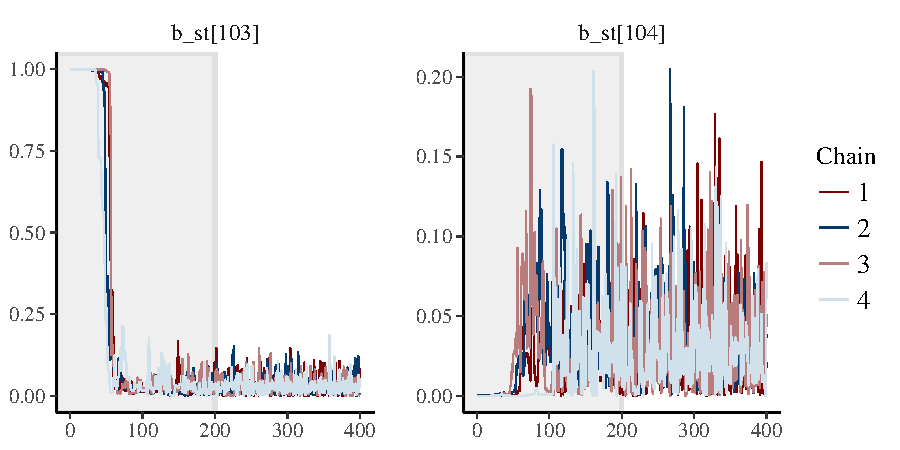
\includegraphics{traceplots.pdf}}
\caption{Draws for two parameters using Stan's HMC algorithm.}
\label{fig:traceplots}
\end{figure*}

In principle extending the SED model of the previous section to Bayesian formalism is straightforward. Given a set of data $\mathcal{D}$ and a vector of parameters $\theta$ Bayes' rule can be written succinctly as \citep{bda3} 

\begin{equation}
\label{eqn:bayesrule}
p(\theta | \mathcal{D}) =  \frac{p(\mathcal{D} | \theta) p(\theta)}{\int p(\mathcal{D} | \theta) p(\theta) \mathrm{d} \theta}
\end{equation}

where $p(\theta)$ is the prior distribution for the parameters, $p(\mathcal{D} | \theta)$ the likelihood of the data given a set of parameters, and $p(\theta | \mathcal{D})$ the posterior distribution of the parameters conditional on the data. The integral in the denominator is usually called the ``evidence'' in Bayesian statistics. The likelihood for this model is given by equation \ref{eqn:like} so all that's needed is a prior. Of course, this is much too simple! Except in special circumstances where the evidence can be calculated analytically or in a low dimensional parameter space where numerical integration is tractable it's necessary to turn to Markov Chain Monte Carlo (MCMC) methods \citep{mcsm} to simulate the posterior. A large number of algorithms have been developed and I have tried several, none of which even approach convergence in any reasonable number of iterations -- that includes the well regarded and superficially promising affine invariant ensemble sampler of \citet{2010gw} implemented by \citet{2013PASP..125..306F} as well as variations of Metropolis-Hastings and Gibbs samplers.

Somewhat by accident while working on another problem I discovered that the implementation of an MCMC algorithm known as Hamiltonian Monte Carlo (HMC) in the probabilistic modeling language Stan \citep{stanlang} produced highly promising results. A detailed description of HMC is well beyond the scope of this paper or the author's competence. A good review at a level accessible to astrophysicists is \citet{2017arXiv170102434B}, or for a more technical treatment \citet{2017arXiv170502891B}. Very briefly HMC solves Hamilton's equations for a Hamiltonian defined as a function of the target distribution augmented with a set of momentum variables. This allows the sampler to make large moves through parameter space at each iteration.

A tiny sample of its performance on a real data example is shown in figure \ref{fig:traceplots} which shows traceplots, that is sequential plots of draws from the posterior for two SSP model contributions in adjacent time bins from fits to one of the IFU spectra discussed later in section \ref{sec:results}. Both of the displayed parameters quickly move away from their initial values and approach stationary distributions well before the end of the warmup period (the shaded interval in the plot). Four independent chains were run in this model and all are well mixed. Note also that instead of taking random walks which would be characteristic of a typical Metropolis-Hastings sampler, parameter values tend to make large jumps at each iteration which indicates efficient exploration of the posterior distribution. This is quite typical behavior: usually all parameters converge to stationary distributions well within the warmup period and only a relatively small number of post-warmup iterations are required for adequate inference. The resulting star formation history estimates always vary continuously at least in distribution and appear to be astrophysically reasonable.

The Stan language is specialized for probabilistic modeling and is most conveniently used from within another system with robust data analysis and manipulation capabilities. Full featured interfaces are provided for \R~ \citep{rstan, rsystem} and Python \citep{pystan}. A command line version is also available, and wrappers around that are provided for several other open source and commercial languages (not including IDL). Motivated mostly by convenience and familiarity the work reported here was done in \R. The same or equivalent tools are available in Python, although a few separate packages for model evaluation just have \R~implementations at the time of writing. Earlier experimental versions of my analysis pipeline were written in Python, and a port of a future version is planned.

Stan programs are highly structured with user defined functions, data, parameters, and the statistical model declared in separate program blocks. There are also optional blocks for transformed data, transformed parameters, and ``generated quantities'' which are any functions of the posterior distribution of interest including posterior predictive checks and log likelihood calculations. The Stan code used for the models reported here is listed in appendix \ref{sec:code}.

This code has a single user defined function to calculate the internal dust attenuation according to the \citet{2001PASP..113.1449C} relation (slightly modified because of a small discontinuity in the published formula). The data section declares the structure of the data but doesn't specify the data itself. That is passed to Stan in an \R~list or Python dict at run time.

The parameters in this model are the SSP model and emission line contributions which are constrained to be non-negative, and the dust optical depth which is also constrained. Here I set a generous upper limit and implicitly give the parameter \texttt{tau} a proper uniform prior on $(0, 3)$. An alternative would be to constrain \texttt{tau} to be nonnegative and provide an informative prior: something like \texttt{tau $\sim$ exponential(1)} might be appropriate.

I did not attempt any kinematic modeling within Stan for this study. Instead I convolve the SSP model spectra with the ML estimated stellar velocity dispersion and similarly create mock emission line spectra as described in the previous section. This is a definite compromise: we would really like to estimate the joint distribution of all parameters of interest rather than a conditional distribution of some parameters on fiducial values of others. The procedure I described in the previous section for creating mock emission line spectra is easily programmed in Stan and exploratory models have been run successfully but execution times are factors of several longer, which puts batch processing of hundreds or thousands of models out of practical reach on a single desktop computer. Fortunately nominal uncertainties in velocity dispersions are generally small and for the galaxies in the sample studied here the estimated velocity dispersions are mostly small as well, so I don't expect the mean star formation histories to be significantly affected. It's likely that dispersions of parameters would be higher if uncertainty in the LOSVD were fully accounted for however.

The other use I make of the ML estimates is to rescale the data by multiplying the SSP model flux values by the maximum SSP contribution and dividing the SSP coefficients by the maximum, making the latter all in $[0, 1]$. Emission line profiles are separately rescaled by multiplying by the maximum emission line contribution in the ML estimate, and again the coefficients are divided by the maximum. The rescaled SSP spectra and emission line profiles are passed to Stan as data along with the observed galaxy fluxes and uncertainties, while the rescaled coefficients and the ML estimate of the dust optical depth are passed as initial values for the parameters with any parameters at boundaries randomly perturbed away from the boundary (this is done for numerical stability). The purpose of these manipulations is to guarantee that the posteriors are unit scaled, that is the posterior means and variances should be $\lesssim 1$. This, along with initializing with parameter values near the optimum helps speed adaptation. This is not an essential step -- there are other effective ways to scale the data and initializing with random parameter values will work, but adaptation is slower and more warmup iterations are required. There is also a greater probability of the sampler getting ``stuck'' in a low probability region of sample space, which can bias posterior inference.

For this investigation I constrained the SSP contributions to lie in $(0, 1)$ as indicated in the example code in appendix \ref{sec:code}. The justification for this is that because the model spectra are highly correlated the SSP model with the largest contribution in the ML solution will \emph{always} converge towards a smaller expected value while others in nearby time or metallicity bins will converge towards larger values. Figure \ref{fig:traceplots} exhibits quite typical behavior: the maximum ML contribution happened to be from a 11.5 Gyr old SSP, while the adjacent 12 Gyr old SSP made 0 contribution. The marginal posterior distributions however are very similar, which is consistent with astrophysical expectations that star formation in a spiral galaxy disk should be slowly declining over cosmic time.

The SSP model contributions are given implicit proper uniform priors on $(0, 1)$. This is not an innocuous choice as it turned out and is likely to change in the future. The emission line contributions are constrained to be nonnegative and are given proper, mildly informative priors. The reason for the different treatment is that emission line contributions are uncorrelated with each other (except for blends like the [O II] lines which will have negatively correlated posteriors) and at most weakly correlated with the stellar contributions. Posteriors for emission lines typically have symmetrical distributions with means very close to their rescaled ML values.

Posterior distributions of any function of the model parameters and input data can be calculated from the posterior samples. I calculate star formation rate and mass growth histories \citep{2012ApJ...745..149L, 2015MNRAS.448.3484M, 2016MNRAS.463.2799I}, emission line fluxes and luminosities, optical depth of attenuation, and summary quantities including present day stellar mass, current (100 Myr timescale) star formation rate, specific star formation rate, light and mass weighted mean stellar age, and mean metallicity. This kind of postprocessing can be done in the generated quantities section of the Stan code or more conveniently in the calling language.

\subsection{Performance on mock data}
\label{sec:mocks}


To test the proposed modeling approach I created a small number of mock data sets. These all have exponentially decaying star formation rates with selectable decay timescale and an optional late time burst in a single age bin. Spectra were constructed from the solar metallicity subset of the MIUSCAT models with Gaussian white noise added to achieve a target SNR. These are rebinned to the same logarithmic wavelength scale as SDSS spectra, convolved with Gaussian velocity profiles, and reddened with a \citet{2001PASP..113.1449C} attenuation curve. No emission line spectra were added for this exercise.

The mock spectra were then modeled with the ML and Stan routines described in the previous two sections using the full set of MIUSCAT SSP templates. Just three simulations are shown here, all with a target SNR $\approx 50$ per pixel. Multiple realizations of some model star formation histories were made and these three were repeated at a target SNR of 15, which is closer to a median SDSS spectrum. No significant differences in posteriors were seen in the repeated runs and the lower SNR runs are qualitatively the same as these, with somewhat higher dispersion posteriors. For these simulations the correct dust optical depths were recovered by the ML routine to $\pm 0.01$ and the stellar velocity dispersions to $\pm 5$ km/sec.

One note of purely computational interest is the Stan simulations converged considerably more slowly than I usually observe with real data models. This seems counterintuitive since the mock data fully conforms to model assumptions while real data almost surely does not. The simulations reported here used twice the number of warmup and post warmup iterations as the real data models in the next section. All graphical and quantitative diagnostics indicated satisfactory convergence.

\begin{figure*}[ht]
\centering
\resizebox{\textwidth}{0.5\textwidth}{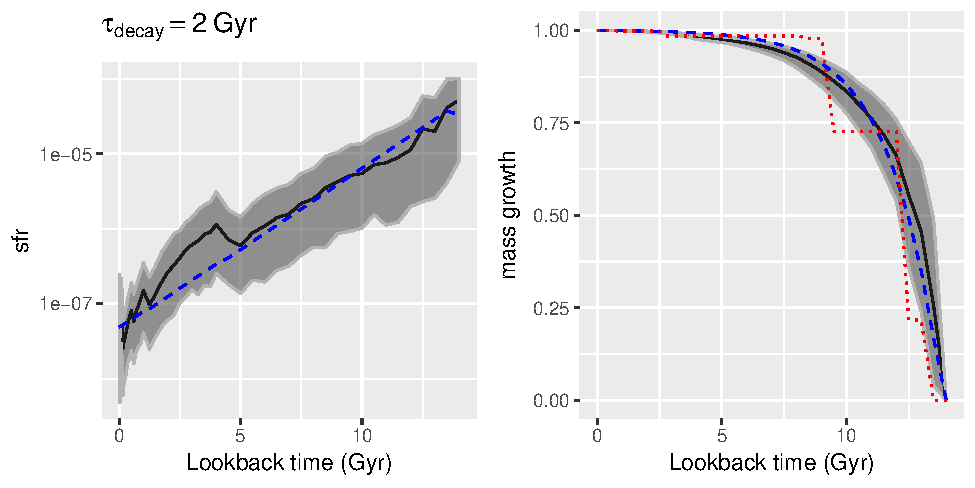
\includegraphics{sf_t2_noburst.pdf}}\vfill
\resizebox{\textwidth}{0.5\textwidth}{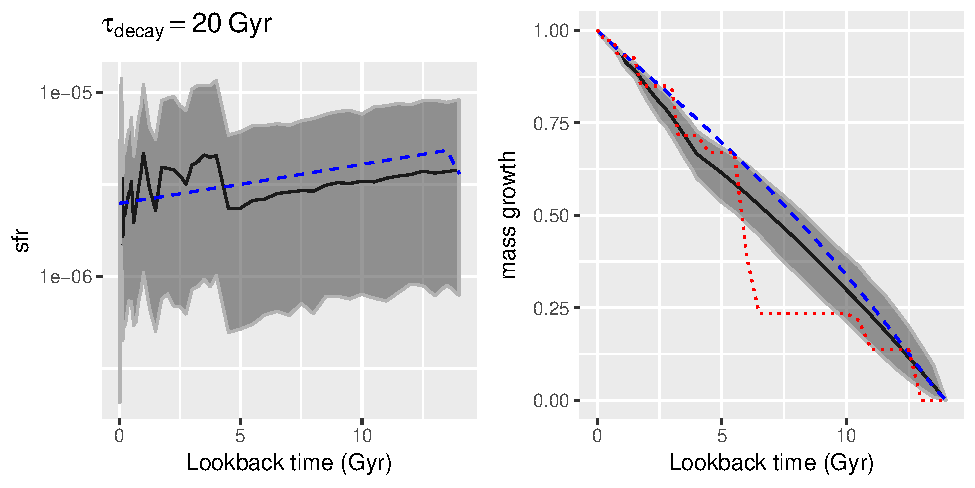
\includegraphics{sf_t20_noburst.pdf}}\vfill
\resizebox{\textwidth}{0.5\textwidth}{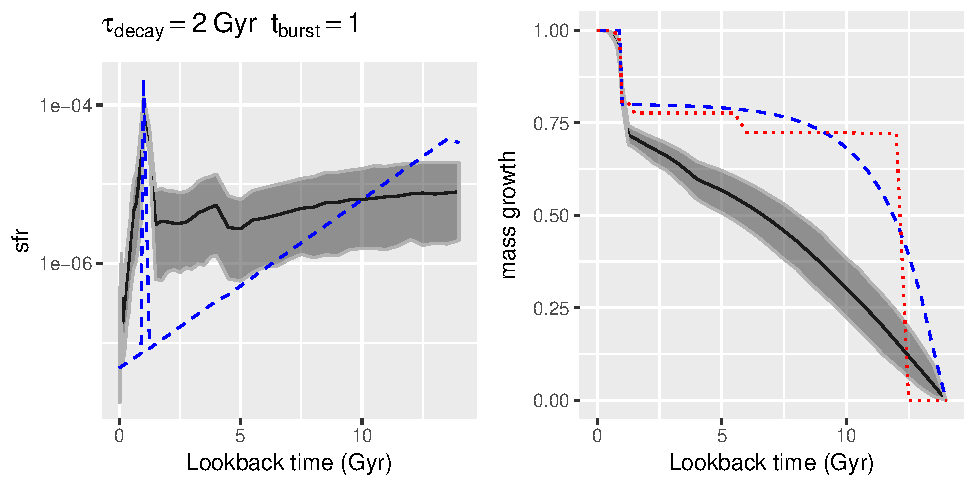
\includegraphics{sf_t2_burst.pdf}}
\caption{Star formation rate and mass growth histories for 3 mock data sets. Star formation rates are arbitrarily scaled.}
\label{fig:mocks}
\end{figure*}


\begin{figure*}[ht]
\centering
\resizebox{\textwidth}{!}{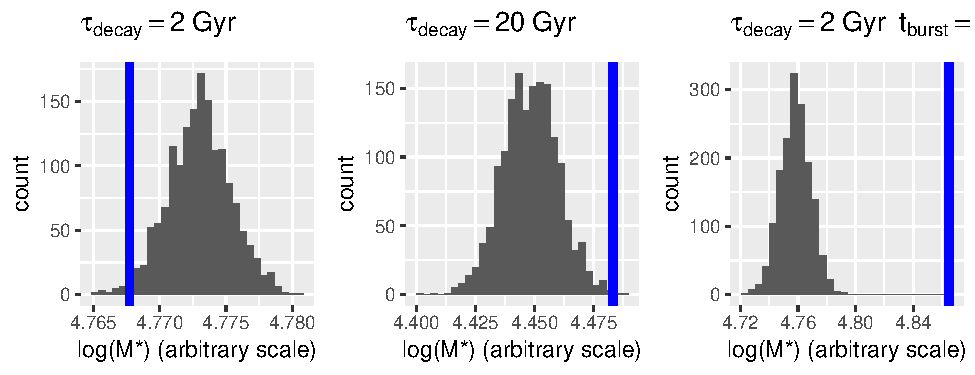
\includegraphics{mstar_mocks.pdf}}
\caption{Posterior distributions of log ``stellar mass''. Blue vertical lines are the actual input values. Scales are arbitrary.}
\label{fig:mstar_mocks}
\end{figure*}

\begin{figure*}[ht]
\centering
\resizebox{\textwidth}{!}{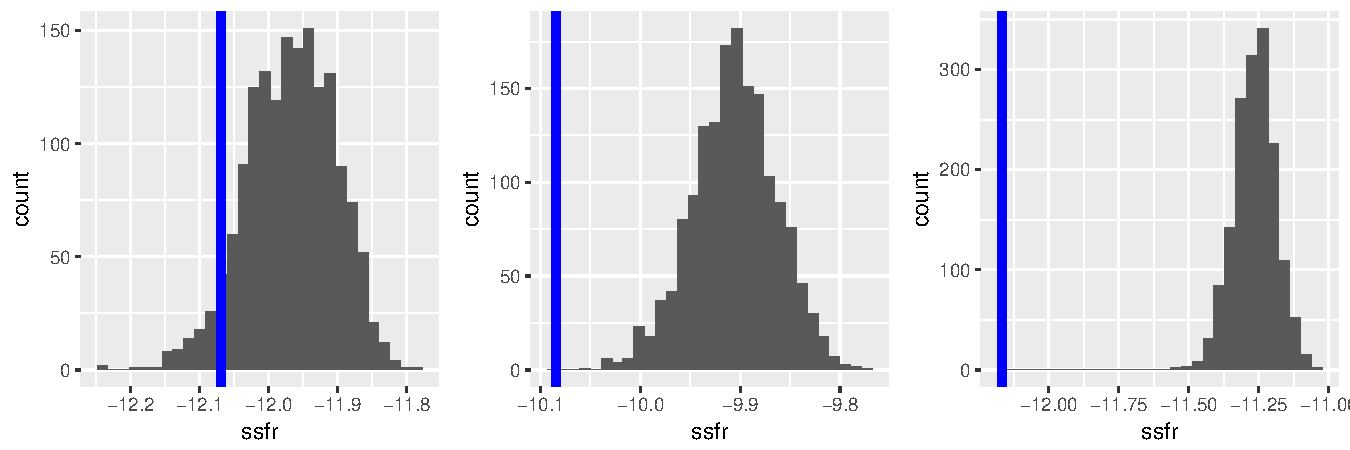
\includegraphics{ssfr_mocks.pdf}}
\caption{Posterior distributions of log specific star formation rate (yr$^{-1}$). Blue vertical lines are the actual input values. Order of the graphs is the same as above.}
\label{fig:ssfr_mocks}
\end{figure*}

\begin{figure*}[ht]
\centering
\resizebox{\textwidth}{!}{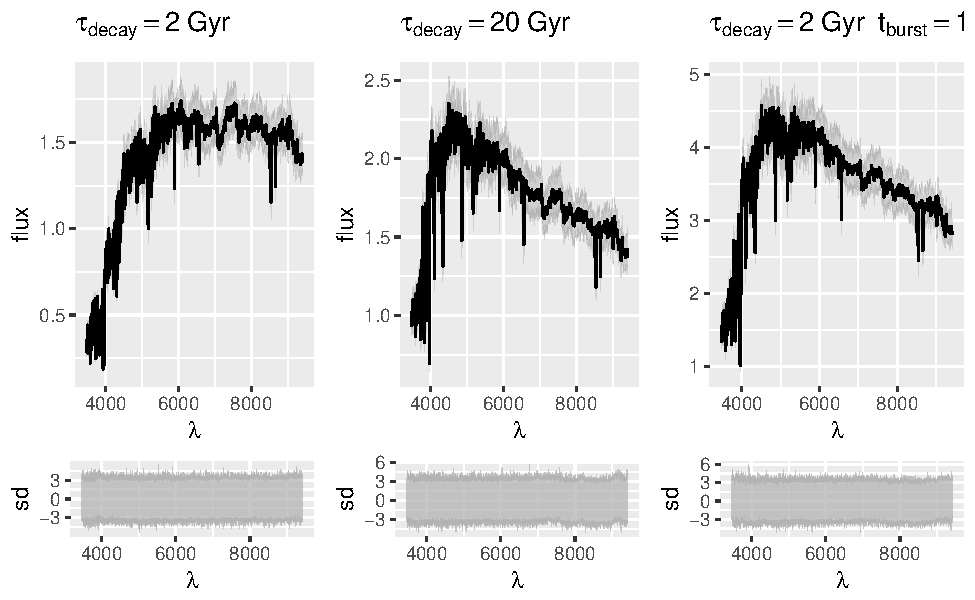
\includegraphics{specfits_mocks.pdf}}
\caption{Posterior predictive fits to the model spectra. Black lines are the error free spectra. Gray ribbons indicate the range of \emph{predicted} flux values. Scales are arbitrary. Lower panes are the residuals of the posterior predictions from the error free spectra in standard deviations.}
\label{fig:specfits_mocks}
\end{figure*}

Some partial results of the simulations are shown in figures \ref{fig:mocks}--\ref{fig:specfits_mocks}. Quantities displayed are arbitrarily scaled, but if the data were real the actual values would be directly proportional. On a logarithmic scale therefore the graphs would simply be offset from the displayed values. The left panes of figure \ref{fig:mocks} show star formation histories, defined as the total stellar mass born in each time bin divided by the width of the bin in years. The right are mass growth histories, defined as the cumulative fraction of the present day stellar mass as a function of lookback time \citep{2012ApJ...745..149L, 2015MNRAS.448.3484M, 2016MNRAS.463.2799I}. The grey ribbons are symmetrical 95\% credible intervals calculated from the posterior samples. Mean values are indicated with black lines. The values for any time bin effectively marginalize over every other parameter, since what is being simulated is the joint posterior density. The actual input values are the blue dashed lines. In the mass growth plots the ML solutions are also shown as red dotted lines.

For the two simulations with smoothly declining star formation rates the posterior credible intervals of SFR cover the actual values for all lookback times. There are hints of systematics in the mass growth histories though, especially in the one with a long decay timescale where the initial mass growth is somewhat slower than the input history with an acceleration in star forming beginning at $\sim 4$Gyr to catch up at late times. Systematics are much more important in the simulated late time starburst with the pre-burst mass growth much more gradual than the input model, slower burst buildup and decay, and more mass formed overall in the burst. On the other hand both the central timing of the burst and peak star formation are accurately captured. Systematics in the mass growth histories lead to systematics in the stellar mass estimates as seen in figure \ref{fig:mstar_mocks}, where the mass of the input history is well outside the range of posterior values for the burst model and far out in the tails of the other two. Other summary measures are also prone to systematic errors, for example the burst simulation has enough lingering star formation to have a specific SFR $\sim$ an order of magnitude larger than the input SFH (figure \ref{fig:ssfr_mocks}).

Despite these biased star formation histories the fits to the data are excellent as seen in figure \ref{fig:specfits_mocks}. These are examples of posterior predictive fits to the spectra, which are created by taking draws of parameter values from the posterior, calculating the resulting spectrum, and adding errors according to the error model which recall is Gaussian with known variances. The black lines in the upper panes are the error free spectrum of the input simulations and the grey clouds are the range of fit values. Residuals in standard deviations shown in the lower panes show slight hints of asymmetry at the red end of the spectra, which probably reflects the loss of information about the old populations in the models. This asymmetry disappears when the actual noisy ``measured'' values are plotted, indicating that the posteriors accurately capture the information content of the data.

Another feature of the models not illustrated here is that SSPs in all 4 metallicity bins make significant contributions in the posterior with similar star formation histories; this is seen in real data as well although sometimes a single metallicity is favored in late time bursts. With that possible exception I see little evidence that chemical enrichment \emph{histories} are strongly constrained by these models.

This still raises the question of why the posterior fails to cover the input star formation histories and for that matter fails to cover the ML solution, which notice straddles the true mass growth histories in each of the simulations. In part this reflects the different goals of Bayesian versus maximum likelihood methods. To first order at least the objective of a Bayesian analysis is to estimate expected values of (functions of) the joint posterior distribution of the parameters. Doing this successfully requires exploring regions of parameter space with high probability mass, which is not necessarily near the modal (maximum likelihood) value. As I noted above the ML solution typically has as few as a handful of nonzero SSP contributors, but many of the zero contributors have significant marginal posterior probability mass at values $> 0$. Perhaps paradoxically then the ML parameter values are often well out in the tails of the marginal posteriors. Because the input model spectra are correlated the parameter posteriors exhibit a complex pattern of correlations as well. In the somewhat artificial late time starburst model this naturally leads to a broader (in distribution) burst.

The prior also plays a role, and this is an issue that needs further investigation. I use proper priors for all parameters, and therefore the prior constitutes a generative model for the data -- that is taking random draws from the prior star formation histories and model spectra can be calculated. The SSP model coefficients are proportional to the stellar mass born in each time bin, while the time bins themselves vary in width becoming narrower at younger ages. This means a typical draw from the prior will have \emph{increasing} star formation rates over cosmic time, which is contrary to the consensus picture that the SFR density of the universe peaked at $z \sim 1-2$. The prior actually does have some effect on the model posteriors. For example there is a persistent jump in mean star formation rates at 4 Gyr that is seen in both the simulations and real data that happens to be one of the breaks in the bin width in the BaSTI isochrone based SSP models used for this study.

A possible replacement for the bounded priors used for this study are truncated (at 0) Gaussians, possibly with scale parameters proportional to SSP bin widths. Preliminary experimentation suggests this reduces the bias in star formation histories and summary measures while still allowing late time starbursts. Whether this improves, or even significantly affects real data inferences has yet to be investigated.

\section{A CASE STUDY}
\label{sec:study}

SDSS-IV MaNGA is a multi-year project to obtain spatially resolved spectroscopy of a planned $\approx 10000$ galaxies in the local universe \citep{2015ApJ...798....7B, 2015AJ....150...19L, 2016AJ....152..197Y}. The first public release, issued in 2016 as part of the 13'th SDSS data release \citep{2016arXiv160802013S} contains spectroscopic measurements for 1390 galaxies with a representative range of morphological types, stellar masses and environments.

Calibrated data products are supplied in two basic forms \citep{2016AJ....152...83L}. ``Row stacked spectra'' (RSS) files contain one spectrum for each IFU fiber and each exposure for a given target. The more familiar data cubes are created from the RSS by interpolation onto a $0.5\arcsec \times 0.5\arcsec$ grid of spaxels with total extent slightly larger than the footprint of the observations. These two file types are supplied with either linear or logarithmic wavelength scales. Since convolution is an important step in the data analysis I use the logarithmically scaled data which have a constant velocity width of $\approx 70$ km/sec per wavelength bin.

While the data cubes are, by design, best suited for visualization for my purposes the RSS files are more useful. The reason quite simply is that the data cubes provide too much data for the MCMC algorithm while adding no information beyond what is in the individual fiber spectra.

The observations collected in the RSS files consist of 3 sets of exposures with the IFU dithered to 3 distinct positions arranged in an equilateral triangle layout, repeated until a target signal to noise ratio is achieved. Thus if there  are $N_{fiber}$ fibers in a given IFU and $N_{exp}$ individual exposures there will be data for $3N_{fiber}$ locations with $N_{exp}/3$ exposures at each position. To create the final data set I perform a weighted stack of all the exposures for each fiber at each position, finally obtaining a set of $3N_{fiber}$ stacked spectra for an object. In detail, if $g_i(\lambda), 1/\sigma_i^2(\lambda)$ are the reported flux and inverse variance for the i'th exposure at wavelength bin $\lambda$ the weighted mean flux for a given fiber/pointing combination is

\begin{equation}
g_{tot}(\lambda) = \sum_{i=1}^{N_{exp}/3} g_i(\lambda)/\sigma_i^2(\lambda)
\end{equation}

with inverse variance

\begin{equation}
1/\sigma_{tot}^2(\lambda) = \sum_{i=1}^{N_{exp}/3} 1/\sigma_i^2(\lambda)
\end{equation}


The exact ordering of spectra within a RSS file isn't fully documented and seems to vary between IFUs although the first $3N_{fiber}$ spectra appear always to comprise one complete set of 3 pointings. I use a K nearest neighbor algorithm to find the remaining $N_{exp}/3 - 1$ spectra for each fiber/pointing combination. The number of fibers per IFU range from 19 to 127, so each data set consists of 57 to 381 stacked spectra and inverse variances. The only other preprocessing step I perform is to correct fluxes and inverse variances for galactic extinction using the E(B-V) value provided in the metadata and the galactic extinction law of \citet{1999PASP..111...63F}.

For this investigation I set a signal to noise threshold (usually median SNR $\ge 5$ over all unmasked wavelength bins) to perform an analysis, with no further attempt at binning by, for example, performing a Voronoi tesselation \citep{2003MNRAS.342..345C}.

The first public data release includes little value added data -- in particular no kinematic measurements are provided other than overall system redshifts. I therefore improvised my own simplified kinematics ``pipeline'' that proceeds in two stages.

In the first stage redshift offsets from the cataloged system redshift are calculated using a template matching procedure very similar to the SDSS \texttt{idlspec2d} pipeline \citep{2011ApJS..193...29A, 2012AJ....144..144B}. The templates at this stage are a set of 15 ``eigenspectra'' from a principal components analysis of $\sim 16000$ SDSS spectra using the matrix factorization algorithm of \citet{2012ApJ...753..122T}. The eigenspectra cover the rest frame wavelength range $3600 \AA \lesssim \lambda \lesssim 8250 \AA$ including the regions of emission lines, which were not masked. This has the important consequence for this task that ionized gas and stellar kinematics must be tightly coupled since only a single redshift measurement is returned. If they are in fact not tightly coupled the returned value will depend on whether emission or absorption lines are more prominent, which can easily vary from one spectrum to another. 

Assuming the sample of galaxies that were used to generate the eigenspectra is representative of the local universe and the basis set of eigenspectra is large enough to span the feature space they will encode information about star formation histories, stellar and gas velocity dispersions, internal attenuation, metallicity variations, etc. Unfortunately it's difficult if not impossible to \emph{decode} the physical information content of a set of empirical eigenspectra, so no physical modeling is done at this stage.

Next the SSP library is regridded to the rest frame of each analyzed spectrum and the ML estimation routine is run to estimate stellar and gas velocity dispersions, optical depth of attenuation, and the NNLS estimates of the SSP and emission line contributions. These solutions are then used to initialize the Stan model as described in section \ref{sec:bayes}, which constitutes the third stage of the analysis pipeline.

I make use of results from all three stages. Velocity fields are calculated from the redshift offsets as $v_{bin} = c\Delta z_{bin}/(1 + z_{sys})$ \citep{2014MNRAS.442.1117D} where $\Delta z_{bin}$ is the estimated offset from the system redshift (which is taken from the metadata) in a given spaxel or fiber. As discussed in section \ref{sec:ml} I subtract the ML estimated emission line contributions from the observed spectra in the process of calculating absorption line indexes, which may have emission line contamination in a sideband or within the central band (particularly in the Balmer lines). This could be done from the Stan model posteriors as well and would have the advantage if using the full posterior sample that the additional uncertainty due to the presence of emission could be calculated. 

The results shown in figures \ref{fig:sfrha} through \ref{fig:mstarssfr} are all derived from the posterior samples returned by Stan. Typically these show posterior means, with posterior standard deviations providing error bars in scatter plots.

\subsection{Case study background}
\label{sec:background}

\begin{table}[h]
\centering
\begin{tabular}{llrrrr}
\hline
mangaid & NED name & $\alpha$ (J2000) & $\delta$ (J2000) & z & $M^*$ \\ 
\hline
1-148068 & MCG +08-19-033 & 156.8057 & 48.2448 & 0.06096 & 10.96 \\ 
1-378164 & UGC 03935 & 114.4559 & 46.3977 & 0.03213 & 10.63 \\ 
1-256002 & 2MASX J11083705+4300151 & 167.1544 & 43.0042 & 0.04989 & 10.16 \\ 
1-210923 & WISE J162105.01+395502.8 & 245.2709 & 39.9174 & 0.03203 & 10.32 \\ 
1-266039 & UGC 09105 & 213.4168 & 43.8666 & 0.03504 & 10.67 \\ 
1-282712 & 2MASX J12314488+4607538 & 187.9369 & 46.1316 & 0.04909 & 9.99 \\ 
\hline
\end{tabular}
\caption{Basic data for the galaxies in this study. The first three are from the red spiral sample of \citet{2010MNRAS.405..783M}, while the second three are from the blue spiral sample. Stellar mass estimates are from the NASA Sloan atlas as retrieved from the MaNGA drpall catalog file.}
\label{table:basedata}
\end{table}

\begin{figure*}[ht]
\centering
\resizebox{0.3\textwidth}{!}{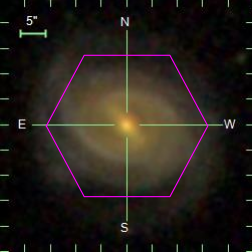
\includegraphics{1_148068.png}}\hfill
\resizebox{0.3\textwidth}{!}{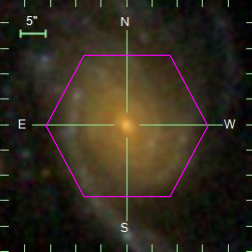
\includegraphics{1_378164.png}}\hfill
\resizebox{0.3\textwidth}{!}{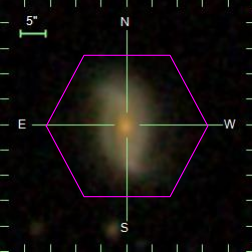
\includegraphics{1_256002.png}}\vfill
\resizebox{0.3\textwidth}{!}{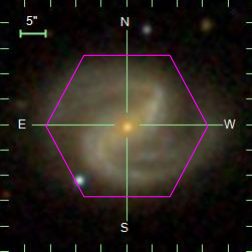
\includegraphics{1_210923.png}}\hfill
\resizebox{0.3\textwidth}{!}{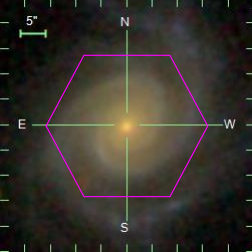
\includegraphics{1_266039.png}}\hfill
\resizebox{0.3\textwidth}{!}{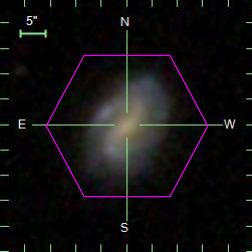
\includegraphics{1_282712.png}}
\caption{SDSS thumbnail images of the galaxies in this study with outlines of the MaNGA coverage. Red sample spirals are in the top row, and blue sample galaxies selected for similar morphologies below. All sets of maps in subsequent figures are displayed in the same order.}
\label{fig:thumbnails}
\end{figure*}

\citetalias{2010MNRAS.405..783M} studied a volume limited sample of 294 red spiral galaxies from the SDSS spectroscopic sample that were selected to

\begin{itemize}
\item
have redshift $0.03 < z < 0.085$ and r band Petrosian absolute magnitude $M_r < -20.17$.
\item
Be high likelihood spirals based on Galaxy Zoo \citep{2008MNRAS.389.1179L} classifications.
\item
Be on the red sequence, which they defined as $(g - r) > 0.63 - 0.02(M_r + 20)$.
\item
Be close to face on and \emph{not} bulge dominated based on a proxy in the SDSS photometry. These criteria were intended to ensure that red colors were intrinsic to the disk starlight and not due to excess dust reddening or a significant and presumably passively evolving spheroidal component.
\end{itemize}

Also selected was a sample of 5139 blue sequence spirals chosen on the same criteria\footnote{the complete catalog is available from the Vizier service at \url{http://vizier.u-strasbg.fr/viz-bin/VizieR-3?-source=J/MNRAS/405/783}.}.

Although \citetalias{2010MNRAS.405..783M} characterized the red sample as ``passive'' both in the title and multiple times in the text they didn't demonstrate or ultimately even claim that the sample is passively evolving in the usually understood sense of having no detectable ongoing star formation. Also, while a number of proxies for star formation were examined no actual estimates of star formation rates or related quantities were presented. The premise that the red spiral sample is passively evolving was criticized by \citet[][C12]{2012A&A...543A.132C} who found based on a combination of GALEX NUV and WISE mid-IR photometry that the majority of the sample are forming stars at normal rates for their stellar masses.

The spiral samples were revisited by \citet[][T13]{2013MNRAS.432..359T} using the VESPA population synthesis code of \citet{2007MNRAS.381.1252T, 2009ApJS..185....1T} to recover star formation histories in broad age bins. They found among other things that red late type spirals, that is the sample of \citetalias{2010MNRAS.405..783M}, have $\sim 1/2$ the recent ($< 0.5$ Gyr) star formation of either early or late type blue spirals while significantly exceeding that of red sequence ellipticals. Whether this conclusion resolves the apparent tension with that of \citetalias{2012A&A...543A.132C} is unclear. The UV-visual derived SSFR-stellar mass relationship exhibits considerable intrinsic and measurement error scatter \citep{2007ApJS..173..267S}, and a deviation from the mean relation of $\approx 0.3$ dex in any single galaxy would be unsurprising. A purely stochastic explanation for a deviation of the sample \emph{mean} of this magnitude seems unlikely given the reported uncertainties in mass fractions, although on shorter timescales $< 100$ Myr the difference between red and blue spirals is less convincingly significant. This would perhaps support the suggestion of \citetalias{2012A&A...543A.132C} that differences in early time mass formation rather than current star formation rate are responsible for the color differences.

\citetalias{2013MNRAS.432..359T} based their analysis entirely on SDSS fiber spectra so we should also consider the possible effect of aperture bias \citep{2005PASP..117..227K} on their results. This would require a larger bias in red spirals than blue to fully reconcile the results of \citetalias{2013MNRAS.432..359T} with the galaxy wide photometry considered by \citetalias{2012A&A...543A.132C}. In fact \citetalias{2010MNRAS.405..783M} found a larger percentage of both bars and AGN emission in the red spiral sample and either of these could be a source of localized feedback suppressing star formation in the inner $\sim$ few kiloparsecs.

Recently \citet{2016arXiv161105932O} have found evidence that the SSFR -- stellar mass relationship has a \emph{trimodal} distribution with a well defined sequence of galaxies having specific star formation rates intermediate between the star forming ``main sequence'' and passively evolving galaxies, and which they argue are slowly transitioning from actively star forming to passive. They specifically cite \citetalias{2013MNRAS.432..359T} as having identified a population of these ``quiescently'' evolving galaxies in the red spiral sample. Similar arguments for the existence of populations slowly transiting through the ``green valley'' have been made for example by \citet{2015MNRAS.450..435S}.

SDSS MaNGA will ultimately be well positioned to address these alternative hypotheses if it achieves its observational goals, but we cannot do so here. A positional cross match with 3\arcsec~ match radius found three members of the red sample in the first MaNGA public release and 37 members of the much larger blue spiral sample. It would be desirable of course to analyze all of the latter, but for purposes of this study I chose 3 blue spirals selected completely subjectively to be as morphologically similar as possible to the 3 red spirals and also to have similar angular sizes. Some basic observational data on the sample is given in table \ref{table:basedata} and cutout images with MaNGA coverage overlaid are in figure \ref{fig:thumbnails}. In the remainder of this paper I will refer to individual objects by their mangaid.

\begin{figure*}[ht]
\resizebox{\textwidth}{!}{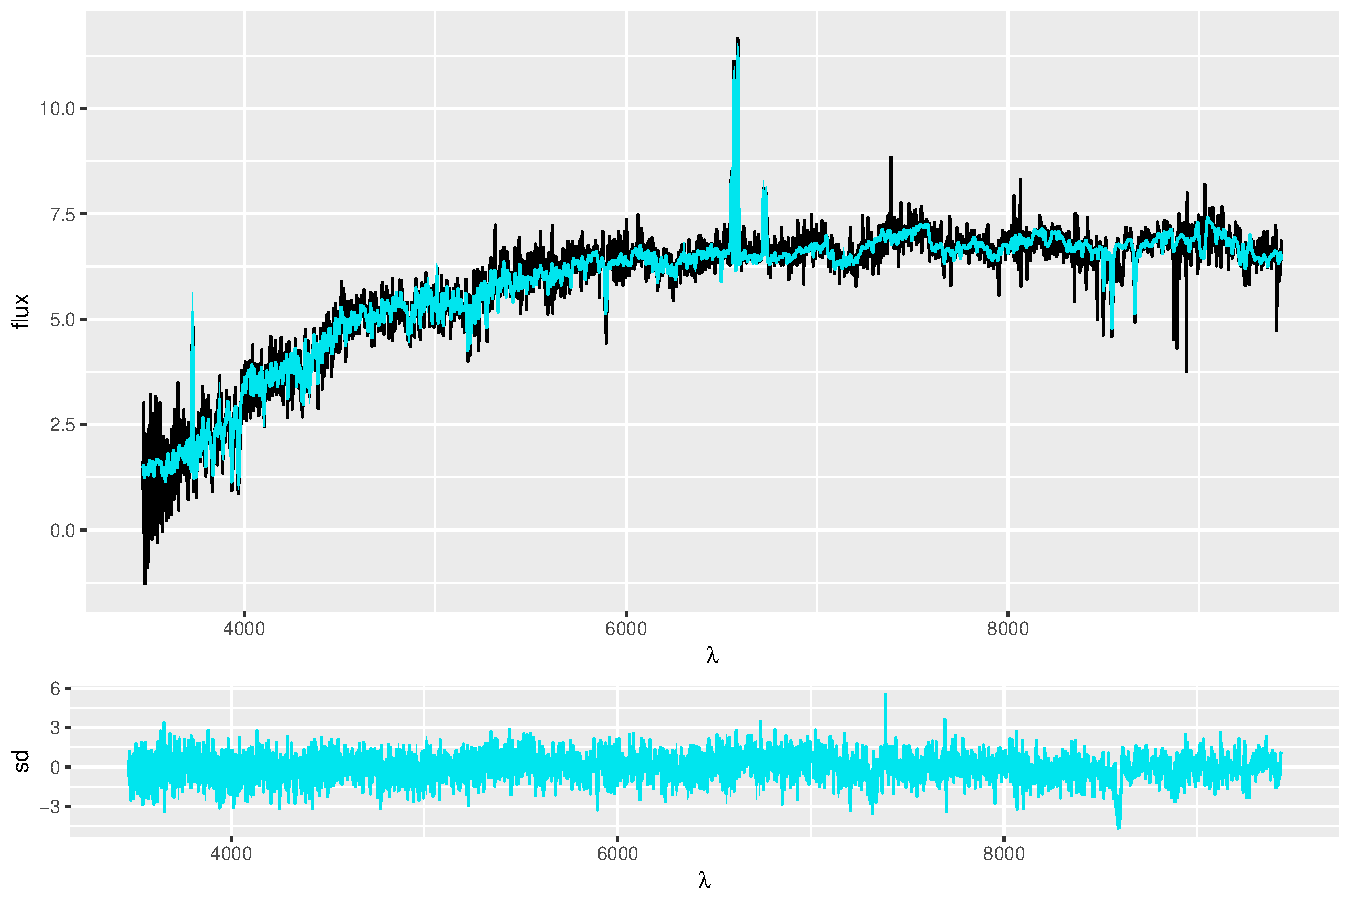
\includegraphics{fit_1_256002-44.pdf}}
\caption{Posterior fit to the spectrum of the central fiber of mangaid 1-256002. Observed values are in black and the model fit in blue. Residuals in standard deviations are shown in the bottom pane.}
\label{fig:specfit}
\end{figure*}

\subsection{Results}
\label{sec:results}

This section presents a number of results from both the ML and Bayesian modeling. The Stan models reported here were fit with a reduced basis set of SSP models with 23 age and 3 metallicity bins, with the lowest metallicity bin of the full set of templates described in section \ref{sec:ml} dropped. This was done to save CPU time -- the execution time for a single Stan model is highly variable but roughly proportional to the number of SSP + emission line templates. Using a reasonably well chosen subset has virtually no effect on fits to the data, but there are occasional differences seen in star formation histories due to the coarser time resolution. A typical fit to the data is shown in figure \ref{fig:specfit}, which shows the estimated noise free spectrum produced by the model posterior for the central fiber of mangaid 1-256002. Compared to the simulations some spectral covariance is evident in this plot, which is due in part to the fact the spectrum is sampled on a finer grid than its resolution and partly perhaps to differences in absolute calibration, metallicity (or metal distribution), or missing ingredients in the SSP models \citep{2013ARA&A..51..393C}. Overall the fit is quite satisfactory with only a small number of conspicuous outliers. This was generally the case with this sample, although night sky subtraction was worse in some spectra than the one displayed here. I do not, by the way, use sigma clipping or other data rejection techniques. In a Bayesian context it's preferable to \emph{model} bad data \citep{2010arXiv1008.4686H}, and this is a possible extension of the current model. The only data excluded were pixels flagged as bad by the MaNGA data processing pipeline or rest frame wavelengths outside the SSP model coverage.

\begin{figure*}[ht]
\centering
\resizebox{0.3\textwidth}{!}{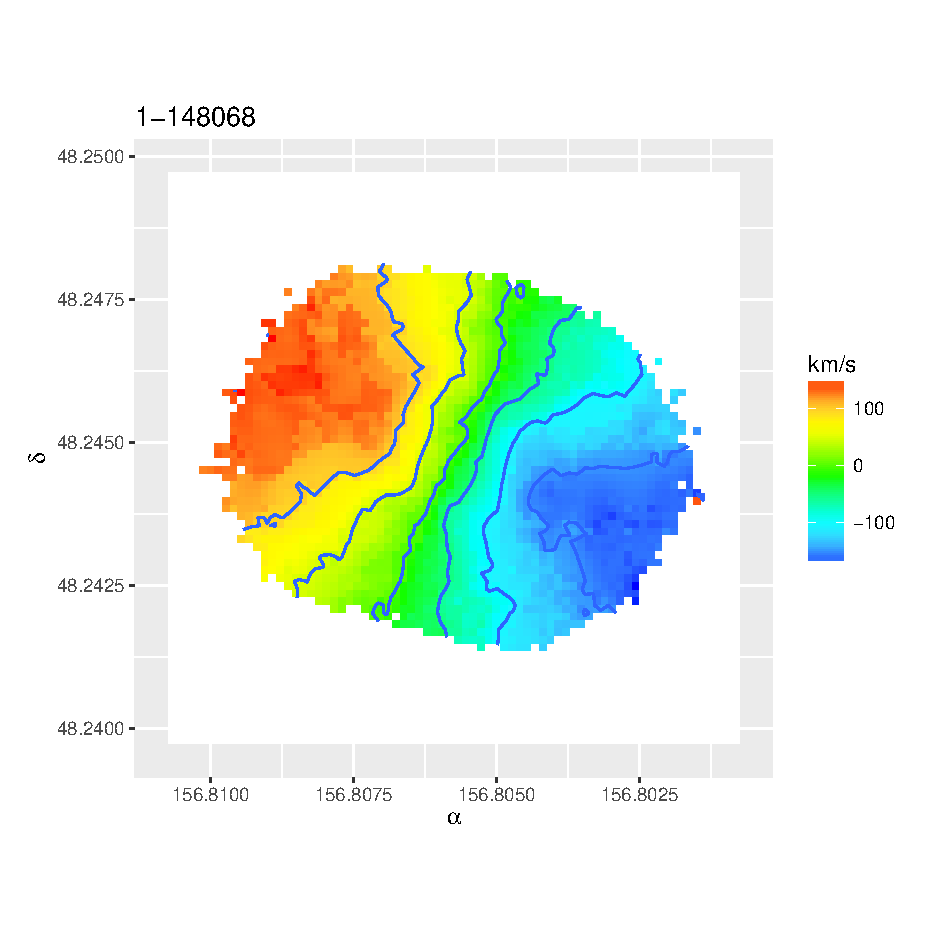
\includegraphics{vf_1_148068.eps}}\hfill
\resizebox{0.3\textwidth}{!}{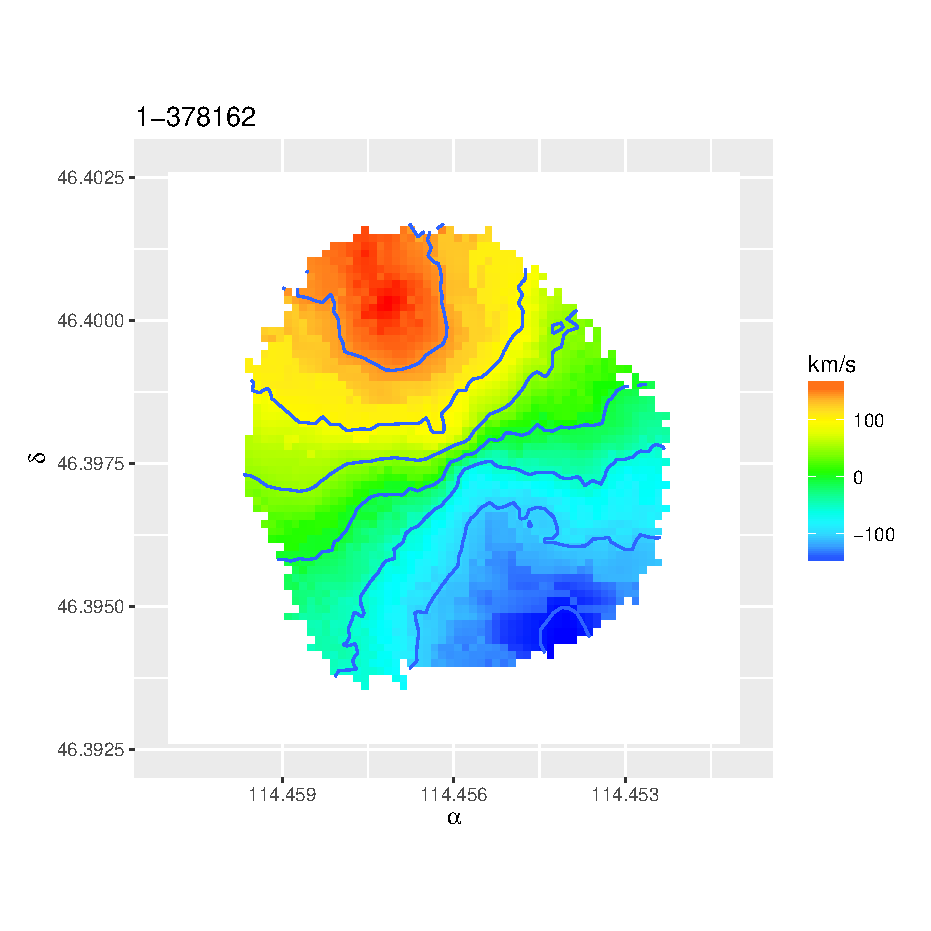
\includegraphics{vf_1_378164.eps}}\hfill
\resizebox{0.3\textwidth}{!}{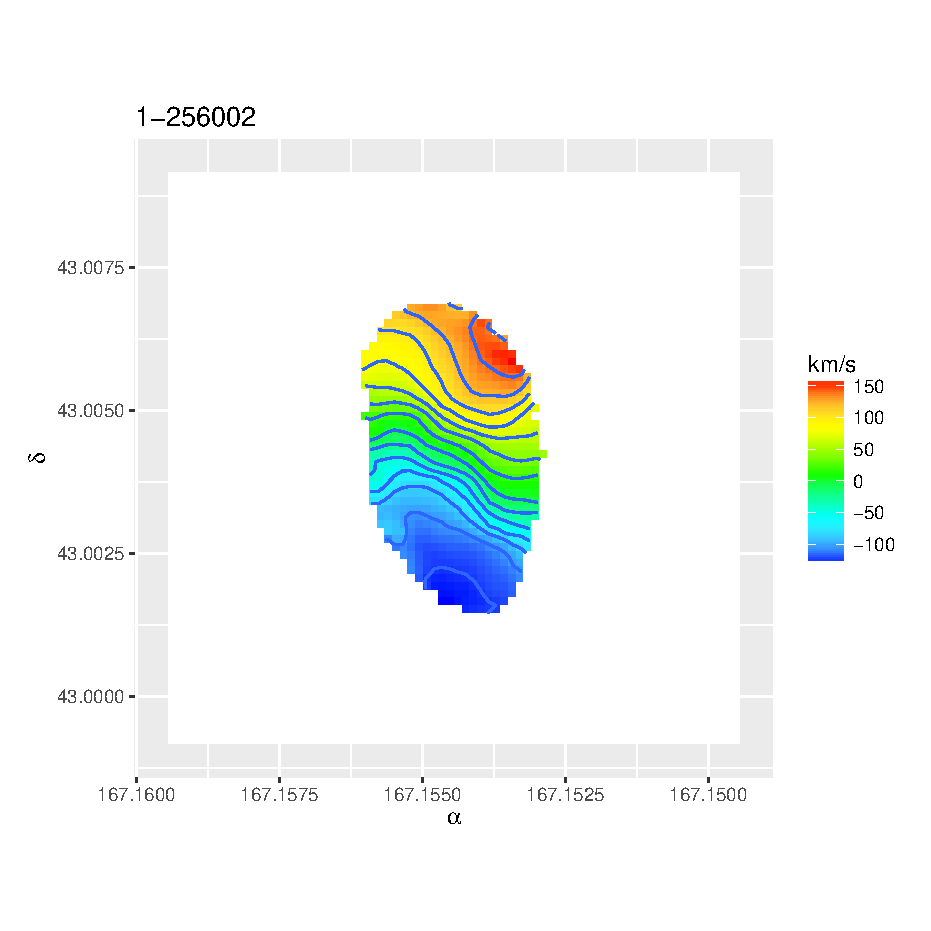
\includegraphics{vf_1_256002.eps}}\vfill
\resizebox{0.3\textwidth}{!}{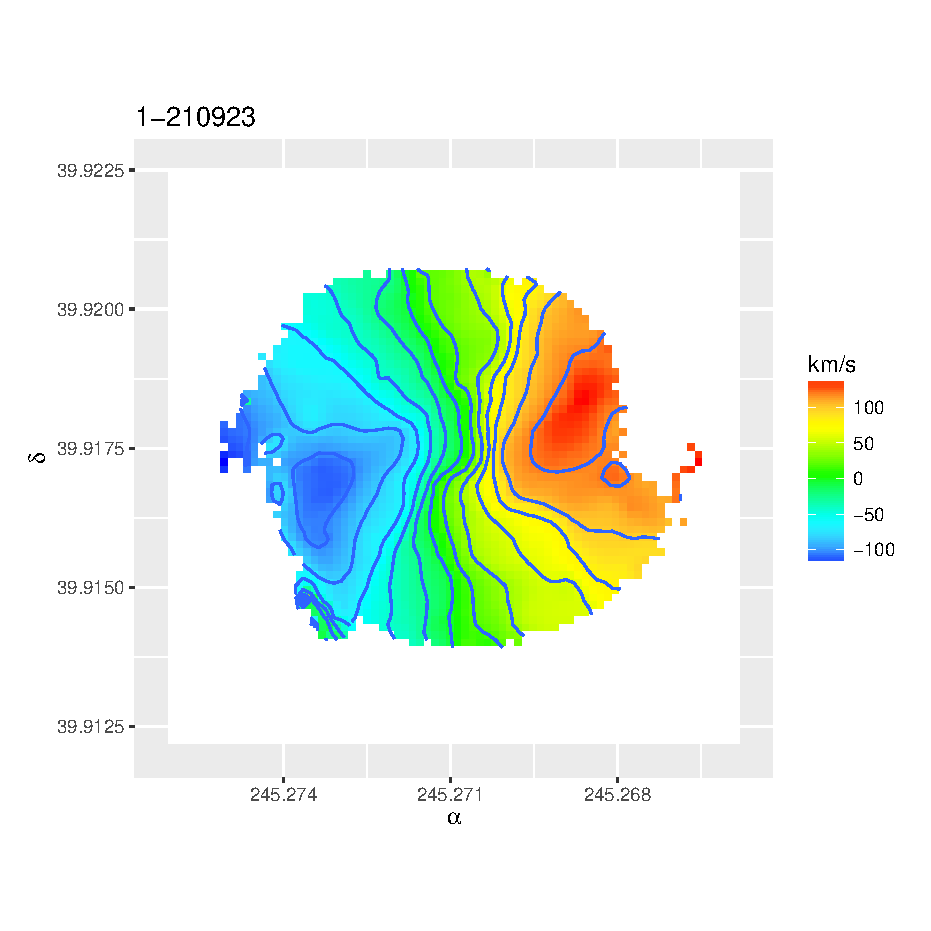
\includegraphics{vf_1_210923.eps}}\hfill
\resizebox{0.3\textwidth}{!}{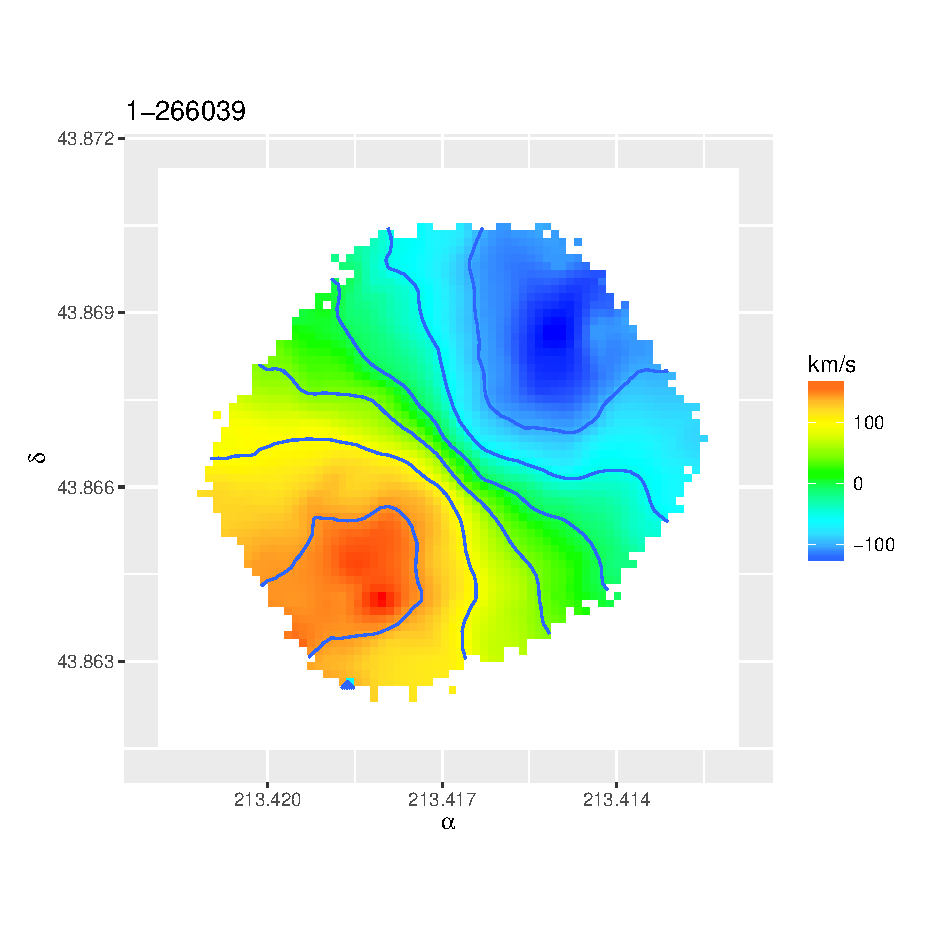
\includegraphics{vf_1_266039.eps}}\hfill
\resizebox{0.3\textwidth}{!}{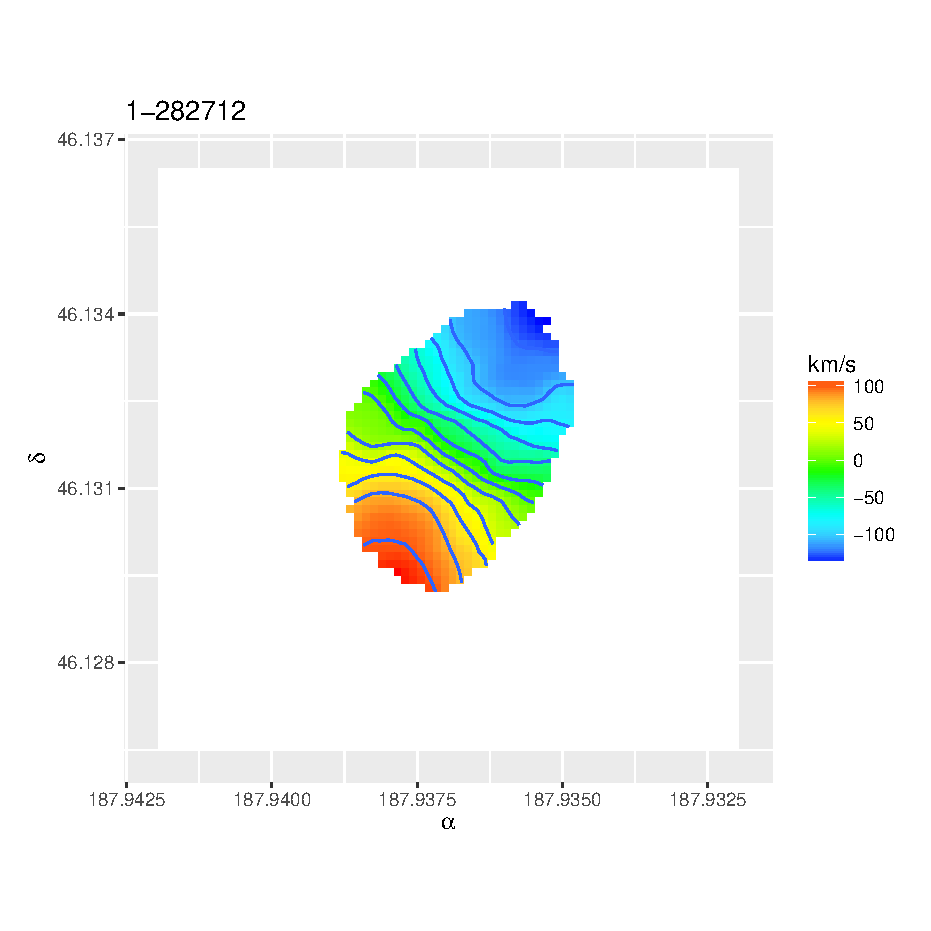
\includegraphics{vf_1_282712.eps}}

\caption{Velocity fields estimated from the data cubes. Ordering of the galaxies in this and all subsequent sets of maps is the same as in Figure \ref{fig:thumbnails}. The mapping of values to colors was performed independently for each object, so scales differ.}
\label{fig:vfs}
\end{figure*}

Many of the results are displayed as maps. For quantities derived from the data cubes these are shown at the $0.5\arcsec \times 0.5\arcsec$ resolution of the spaxels. To create maps of results from fits to the RSS files I do thin plate spline fits to the data, then interpolate on a finer grid than the data cubes. This produces perceptually smoother, less pixellated maps than the data cubes, but small scale details are surely spurious since the true resolution is no better than the fiber diameter of 2\arcsec and is typically somewhat worse. Of course this is true of the data cubes as well. The routine used for interpolation will by default not extrapolate outside the convex hull enclosing points with measurements so the resulting maps are irregular polygons. 

To facilitate comparison with the optical images all maps are displayed at the same spatial scale with the same boundaries as the data cubes which are in turn slightly larger than the IFU footprint. The mapping of values to colors on the other hand was done independently for each galaxy, so scales vary.

The first two maps are calculated from the data cubes. Figure \ref{fig:vfs} are velocity fields, displayed as offsets in km/sec. from the system redshift provided in the metadata. All galaxies are clearly rotating as expected from their morphologies. We can also infer that stars and ionized gas are tightly coupled in all of these systems -- the template matching procedure I described at the beginning of this section fails to produce coherent rotation curves in systems with counterrotating gas and dust, which are not uncommon even in the small sample of MaNGA galaxies available in the first data release \citep{2016MNRAS.463..913J}.

\begin{figure*}[ht]
\centering
\resizebox{0.3\textwidth}{!}{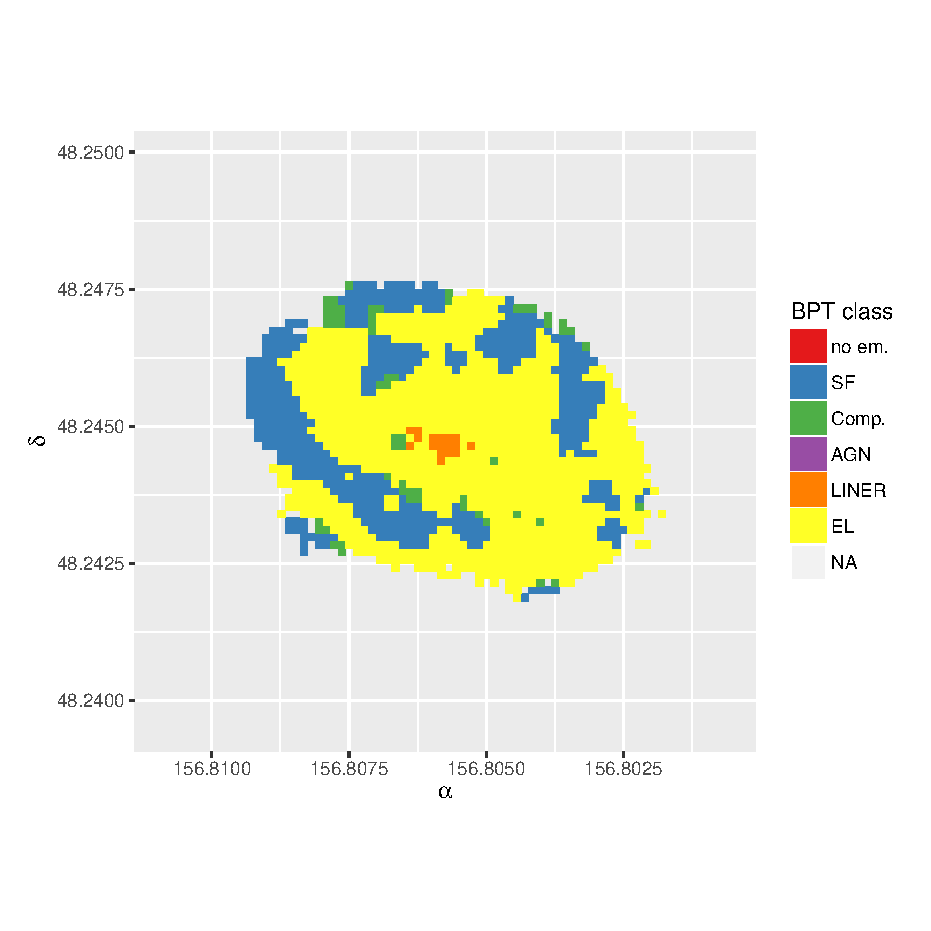
\includegraphics{bpt_1_14.eps}}\hfill
\resizebox{0.3\textwidth}{!}{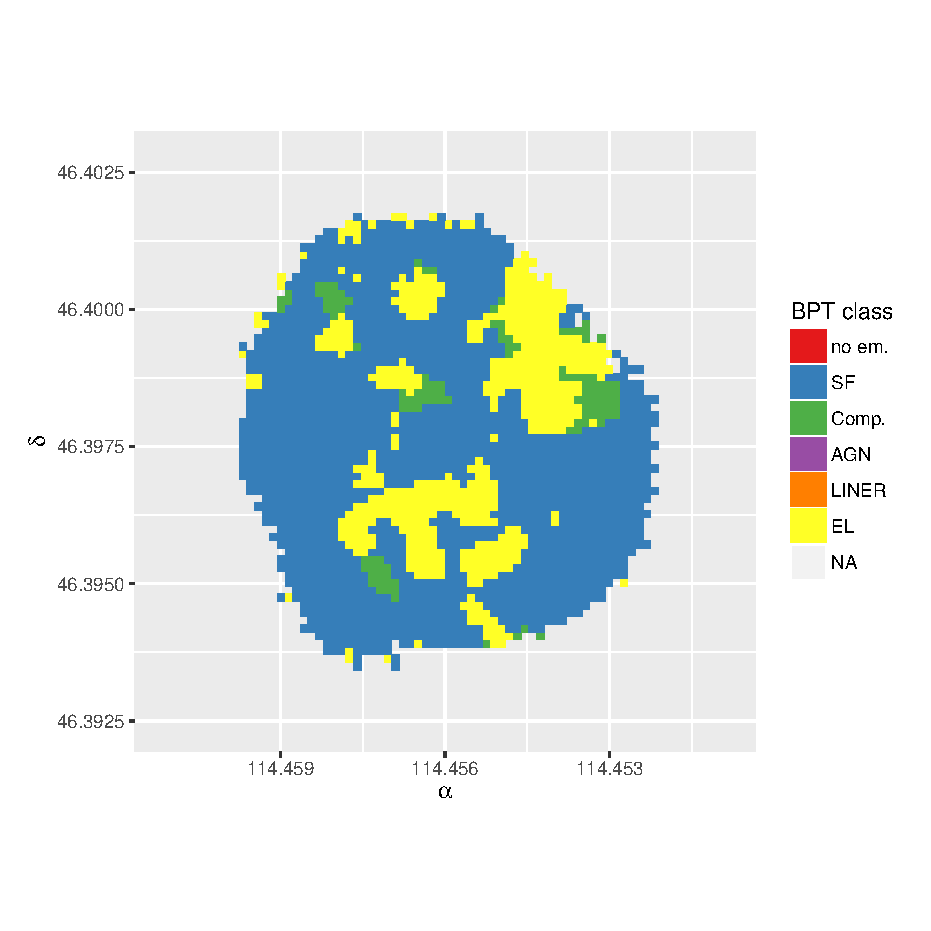
\includegraphics{bpt_1_37.eps}}\hfill
\resizebox{0.3\textwidth}{!}{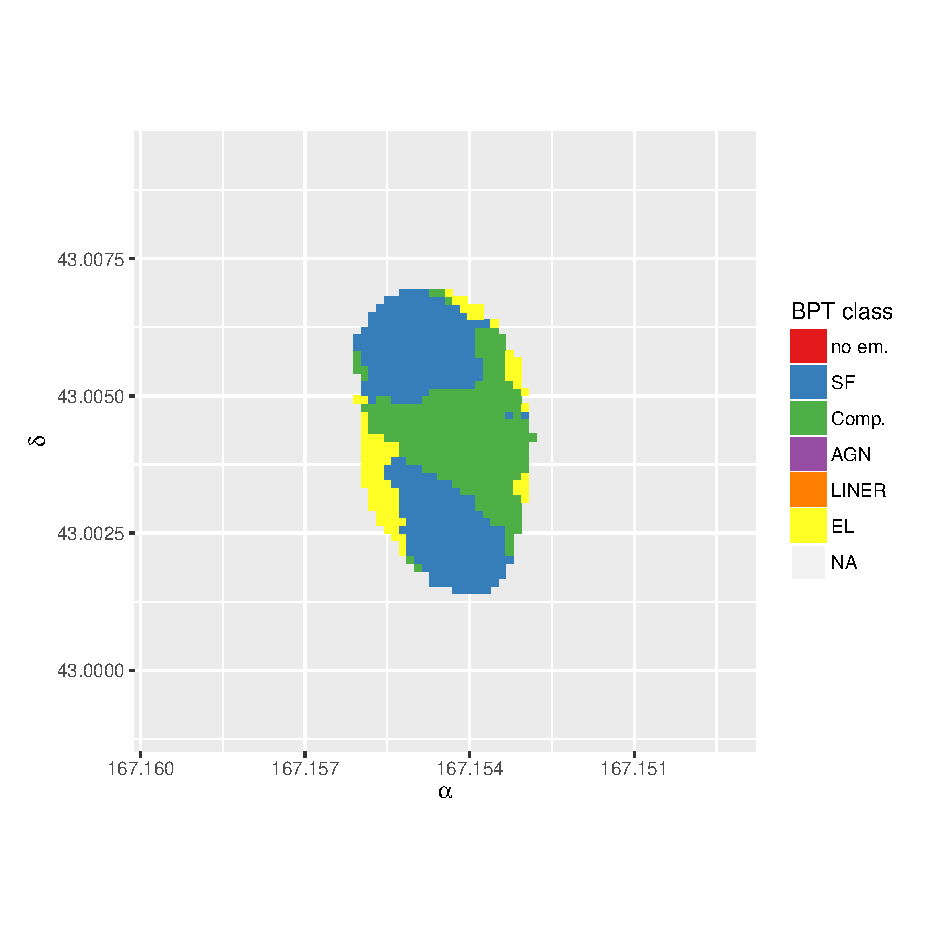
\includegraphics{bpt_1_25.eps}}\vfill
\resizebox{0.3\textwidth}{!}{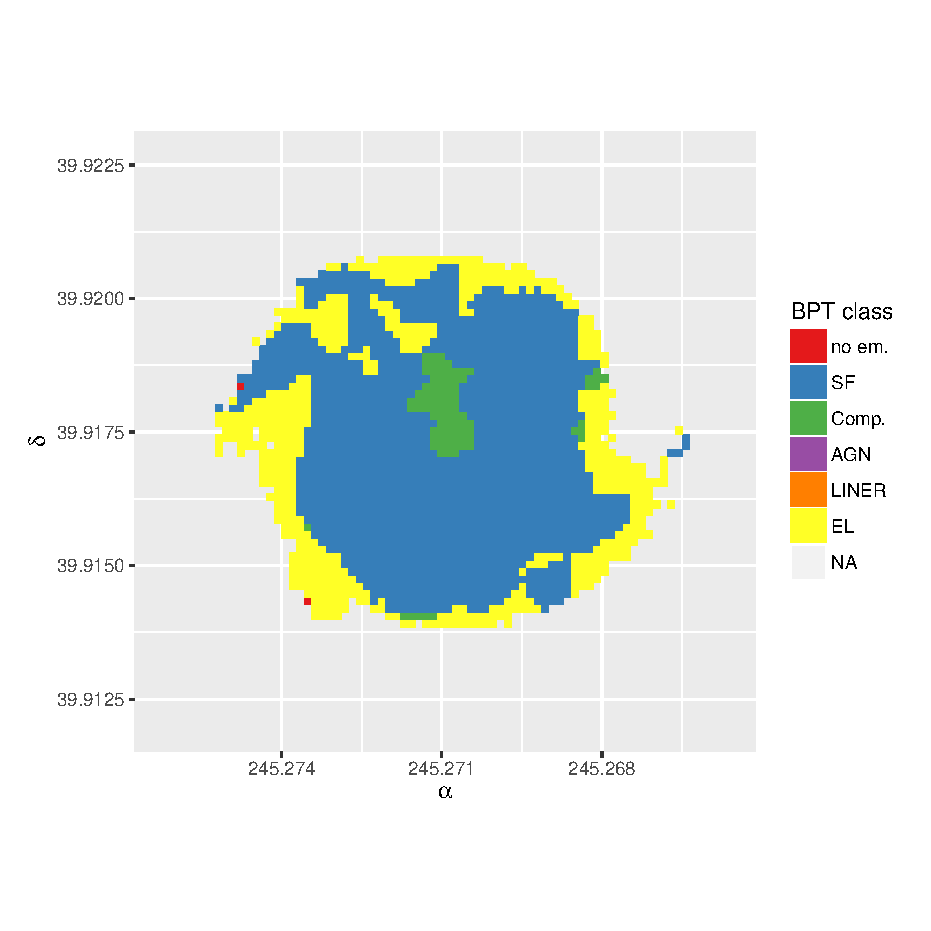
\includegraphics{bpt_1_21.eps}}\hfill
\resizebox{0.3\textwidth}{!}{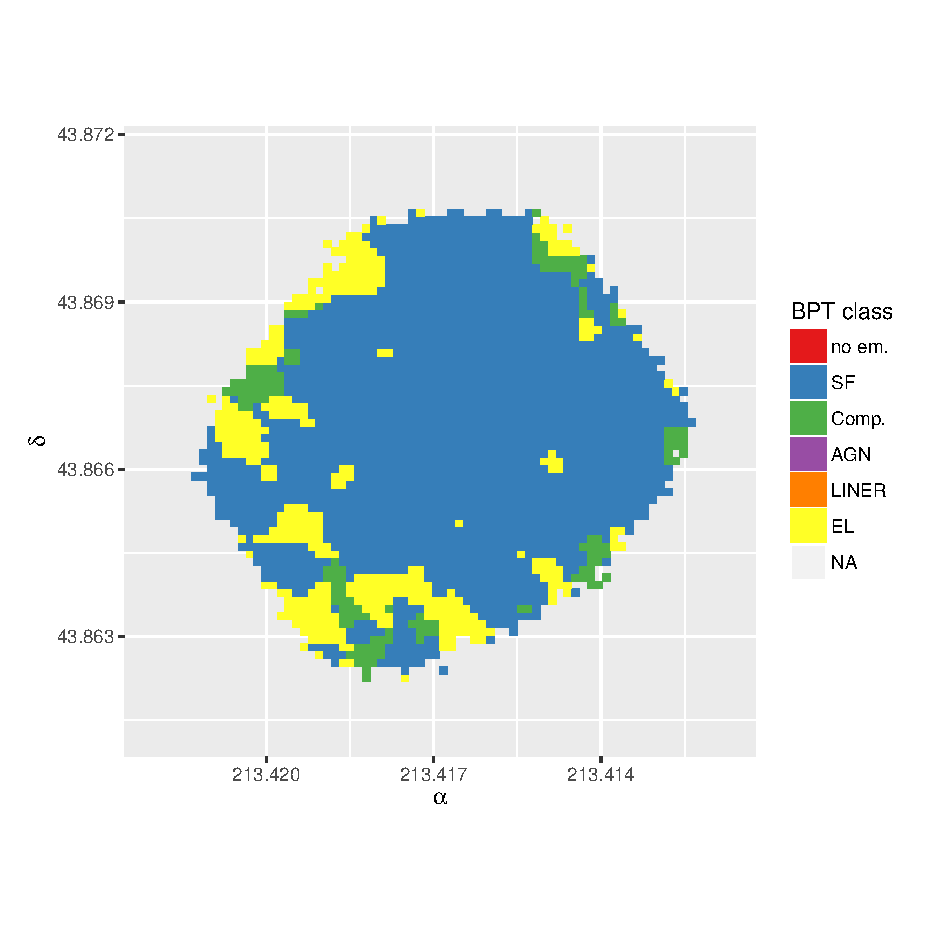
\includegraphics{bpt_1_26.eps}}\hfill
\resizebox{0.3\textwidth}{!}{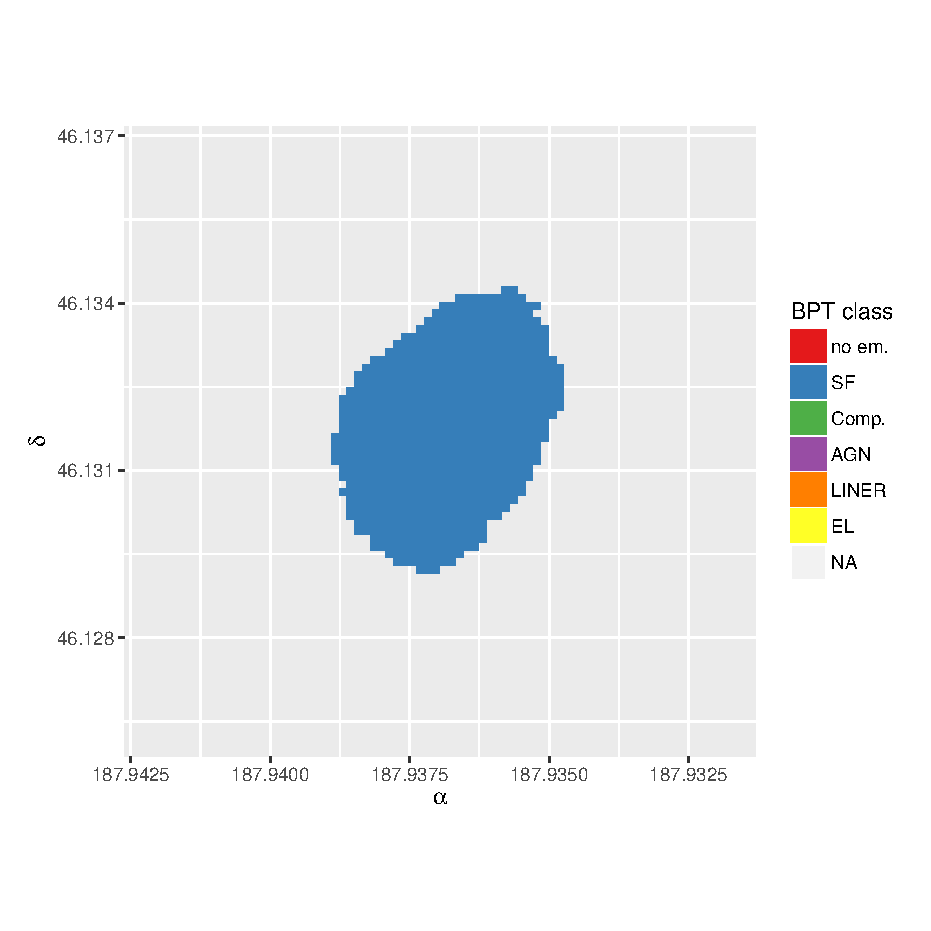
\includegraphics{bpt_1_28.eps}}

\caption{Maps of BPT class from emission line fits to the data cubes. These are based on the ratios [N II]/H$\alpha$ and [O III]/H$\beta$ only.}
\label{fig:bpt}
\end{figure*}


Emission line BPT \citep{1981PASP...93....5B} diagnostic classifications are shown in figure \ref{fig:bpt}. These are based on the ratios [N II]/H$\alpha$ and [O III]/H$\beta$ only and use the commonly adopted demarcation lines of \citet{2003MNRAS.346.1055K} between starforming, ``composite'', and AGN line ratios, and that of \citet{2007MNRAS.382.1415S} to mark the Seyfert-LINER divide. In addition to these spectra with at least one firm ($> 3\sigma$) detection of these lines or [O II] 3727-3729 but not all 4 needed for BPT classification are classified (E)mission (L)ine to distinguish these from spectra with no detected emission at all (which are absent from this sample).

Much recent attention has been given to the observation that LINER like line ratios are often spatially extended \citep[for example][]{2016MNRAS.461.3111B, 2016MNRAS.462.1826H} and not due to ionization by an AGN. Only one galaxy in this sample, mangaid 1-148068, shows any LINER emission and although it appears slightly extended in figure \ref{fig:bpt} only a single fiber spectrum covering the nuclear region falls in the LINER region, therefore this galaxy actually does host a low intensity AGN.

In contrast spectra that fall in the ``composite'' region of the BPT diagram are widely scattered, not necessarily associated with central regions, and always adjacent to regions with either starforming line ratios or weak emission in all galaxies in this sample except 1-282712, which has starforming line ratios throughout. The composite designation was coined by \citet{2004MNRAS.351.1151B} to denote the region between the empirically determined starforming boundary of \citet{2003MNRAS.346.1055K} and the earlier theoretical boundary based on photoionization models of \citet{2001ApJ...556..121K} which they argued was due to a combination of an AGN and starforming regions. This interpretation was widely if not unanimously accepted \citep{2010MNRAS.403.1036C}, but it can't be correct for the majority of spectra in this sample. Recent studies show that other excitation mechanisms including shocks \citep{2011ApJ...734...87R, 2016ApJS..224...38A} and photoionization by hot evolved stars \citep{2008MNRAS.391L..29S} produce emission line ratios falling in the composite and LINER regions. Given that star formation in present day spiral galaxies is generally localized \citep{2012ARA&A..50..531K} it's likely that composite region spectra are (perhaps temporarily) retired areas \citep{2010MNRAS.403.1036C} with currently weak star formation.

\begin{figure*}[ht]
\centering
\resizebox{\textwidth}{!}{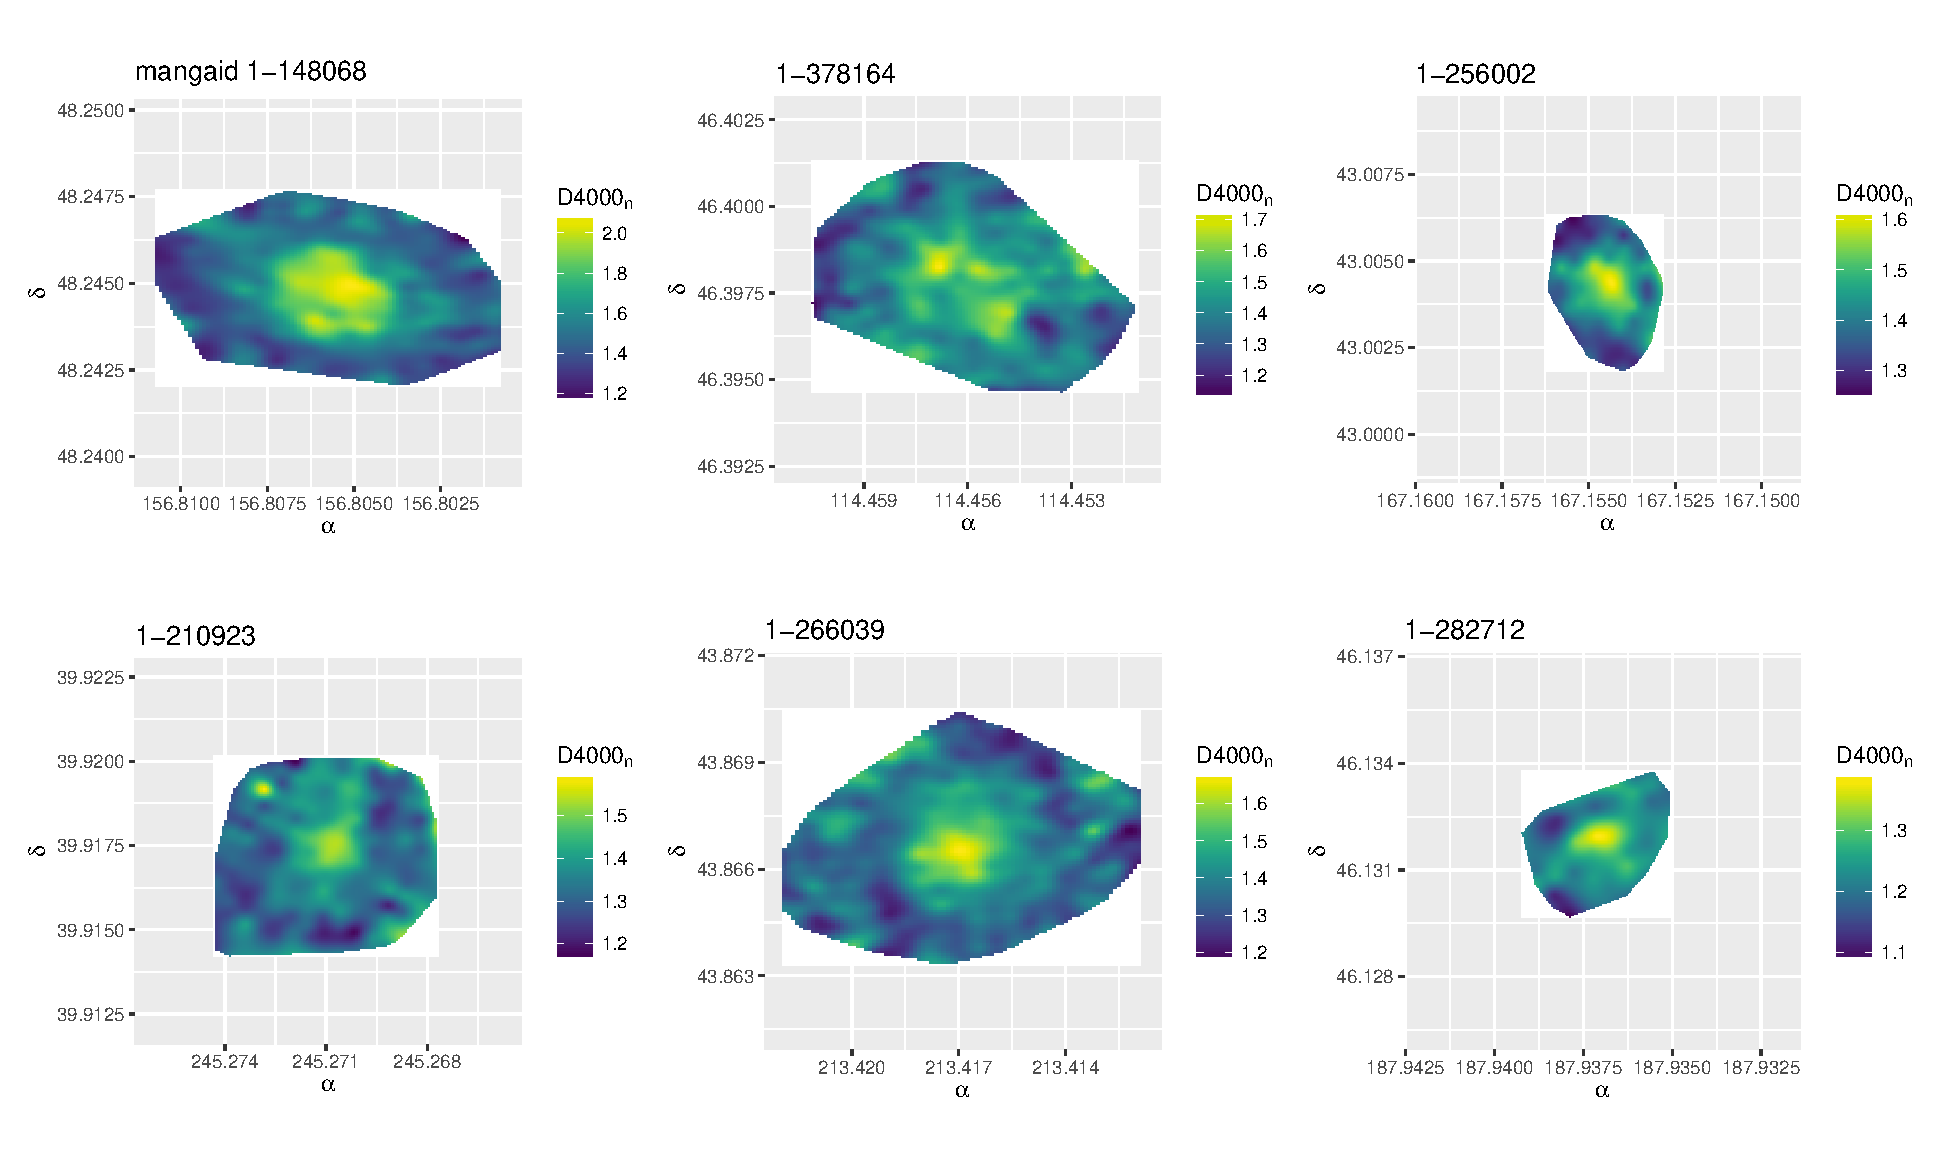
\includegraphics{d4000maps.eps}}
\caption{4000 {\AA} break strength $D4000_n$.}
\label{fig:d4000maps}
\end{figure*}

\begin{figure*}[ht]
\centering
\resizebox{\textwidth}{!}{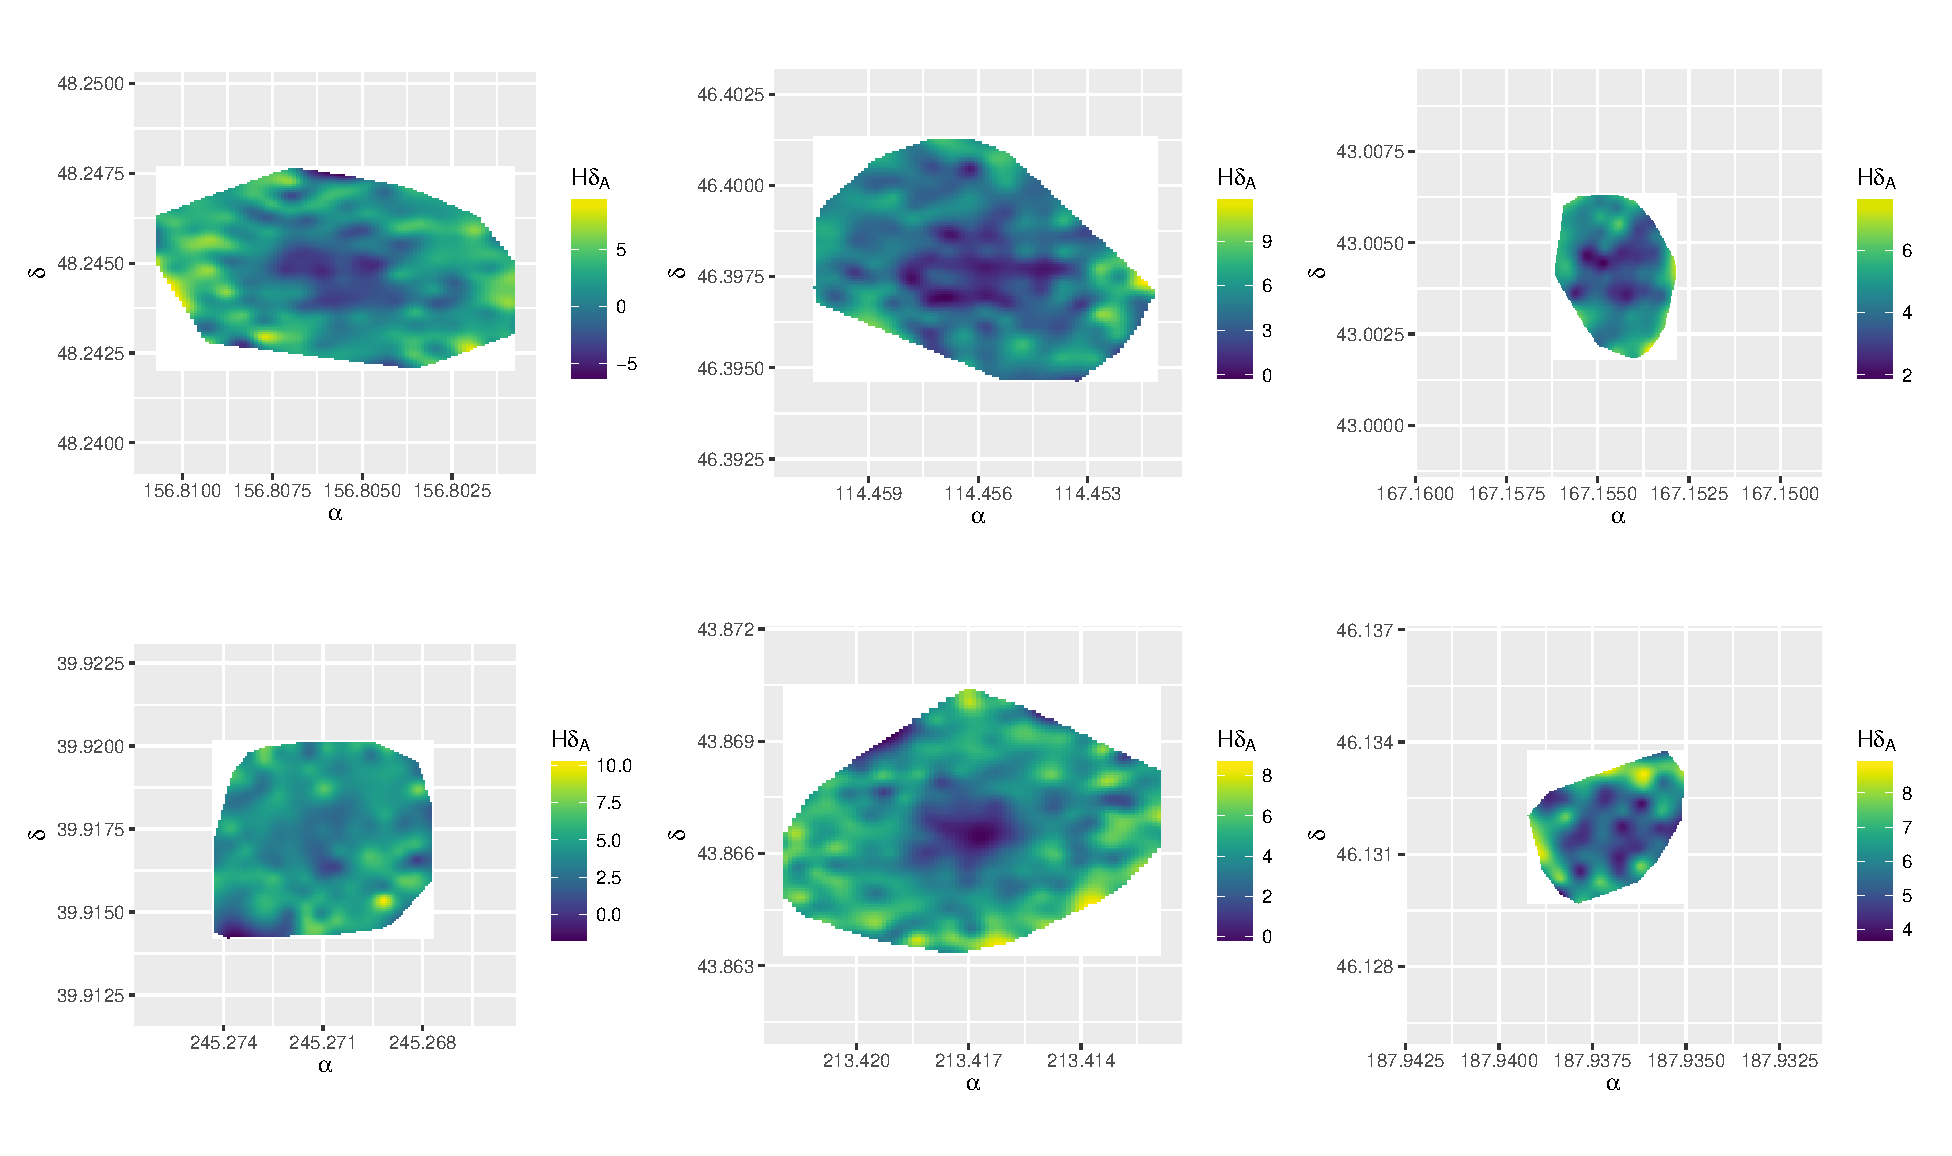
\includegraphics{hdeltamaps.eps}}
\caption{Pseudo-Lick index $H\delta_A$ EW ({\AA}).}
\label{fig:hdeltamaps}
\end{figure*}

Two of the most widely used observational quantities measured in optical spectra are the 4000\AA~ break strength and the Balmer H$\delta$ absorption line equivalent width, which are shown for our sample in figures \ref{fig:d4000maps}, \ref{fig:hdeltamaps}, and \ref{fig:d4000hd}. These provide complementary information about evolutionary state. In coeval stellar populations D$4000_n$ is sensitive to stellar age, with some sensitivity to metallicity at older ages. In composite populations it measures the relative contributions of young and old populations and as such serves as a proxy for specific star formation rate \citep{2004MNRAS.351.1151B}. Balmer absorption line strength is sensitive to the presence of intermediate mass stars and is often interpreted as measuring the burstiness of recent star formation, although ordinary starforming galaxies also have relatively large H$\delta$ indexes.

In this sample the largest values of D4000 and hence oldest populations on average are generally centrally concentrated, consistent with the standard picture of inside out mass growth. The exception here is the non-barred red sample galaxy 1-378164, where the largest values are in an irregular ring surrounding the nucleus. Conversely the largest H$\delta$ equivalent widths are farther out in the disks, primarily in interarm regions.

\begin{figure*}[ht]
\centering
\resizebox{\textwidth}{!}{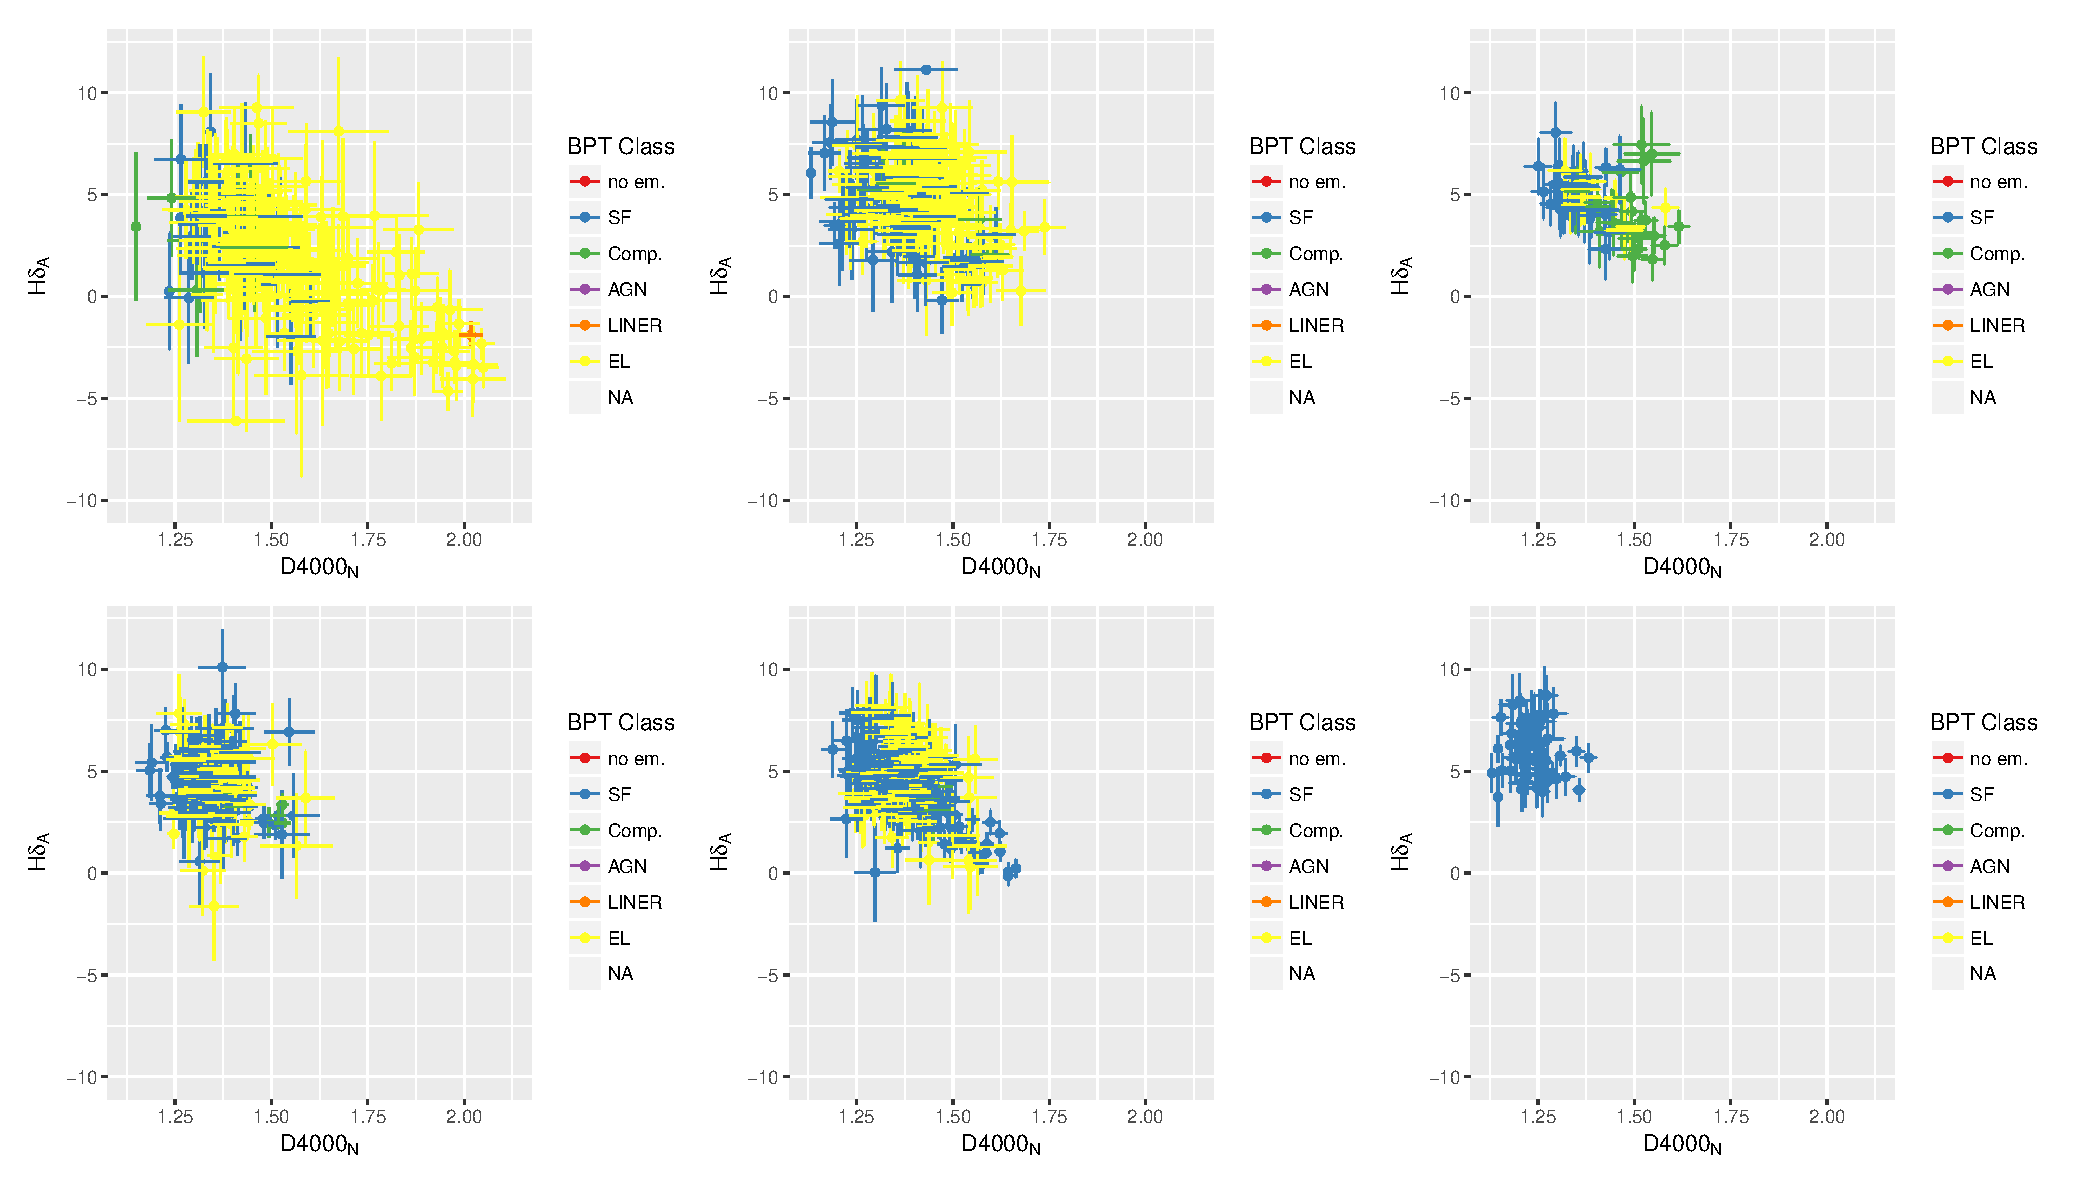
\includegraphics{d4000hd.eps}}
\caption{The $H\delta_A, D4000_n$ plane. Points are color coded by BPT class.}
\label{fig:d4000hd}
\end{figure*}

The red barred spiral 1-148068 is quite remarkable in having nearly the full range of values in the D$4000_n$ - H$\delta_A$ plane (upper left pane of figure \ref{fig:d4000hd}) as a large random sample of galaxies, although the detailed distribution is different. This indicates a wide range of evolutionary states, from actively starforming regions to old and passively evolving. The nucleus is near the lower right, passively evolving edge of the distribution, along with fibers sampling the bar and innermost arms.

\begin{figure*}
\resizebox{0.5\textwidth}{!}{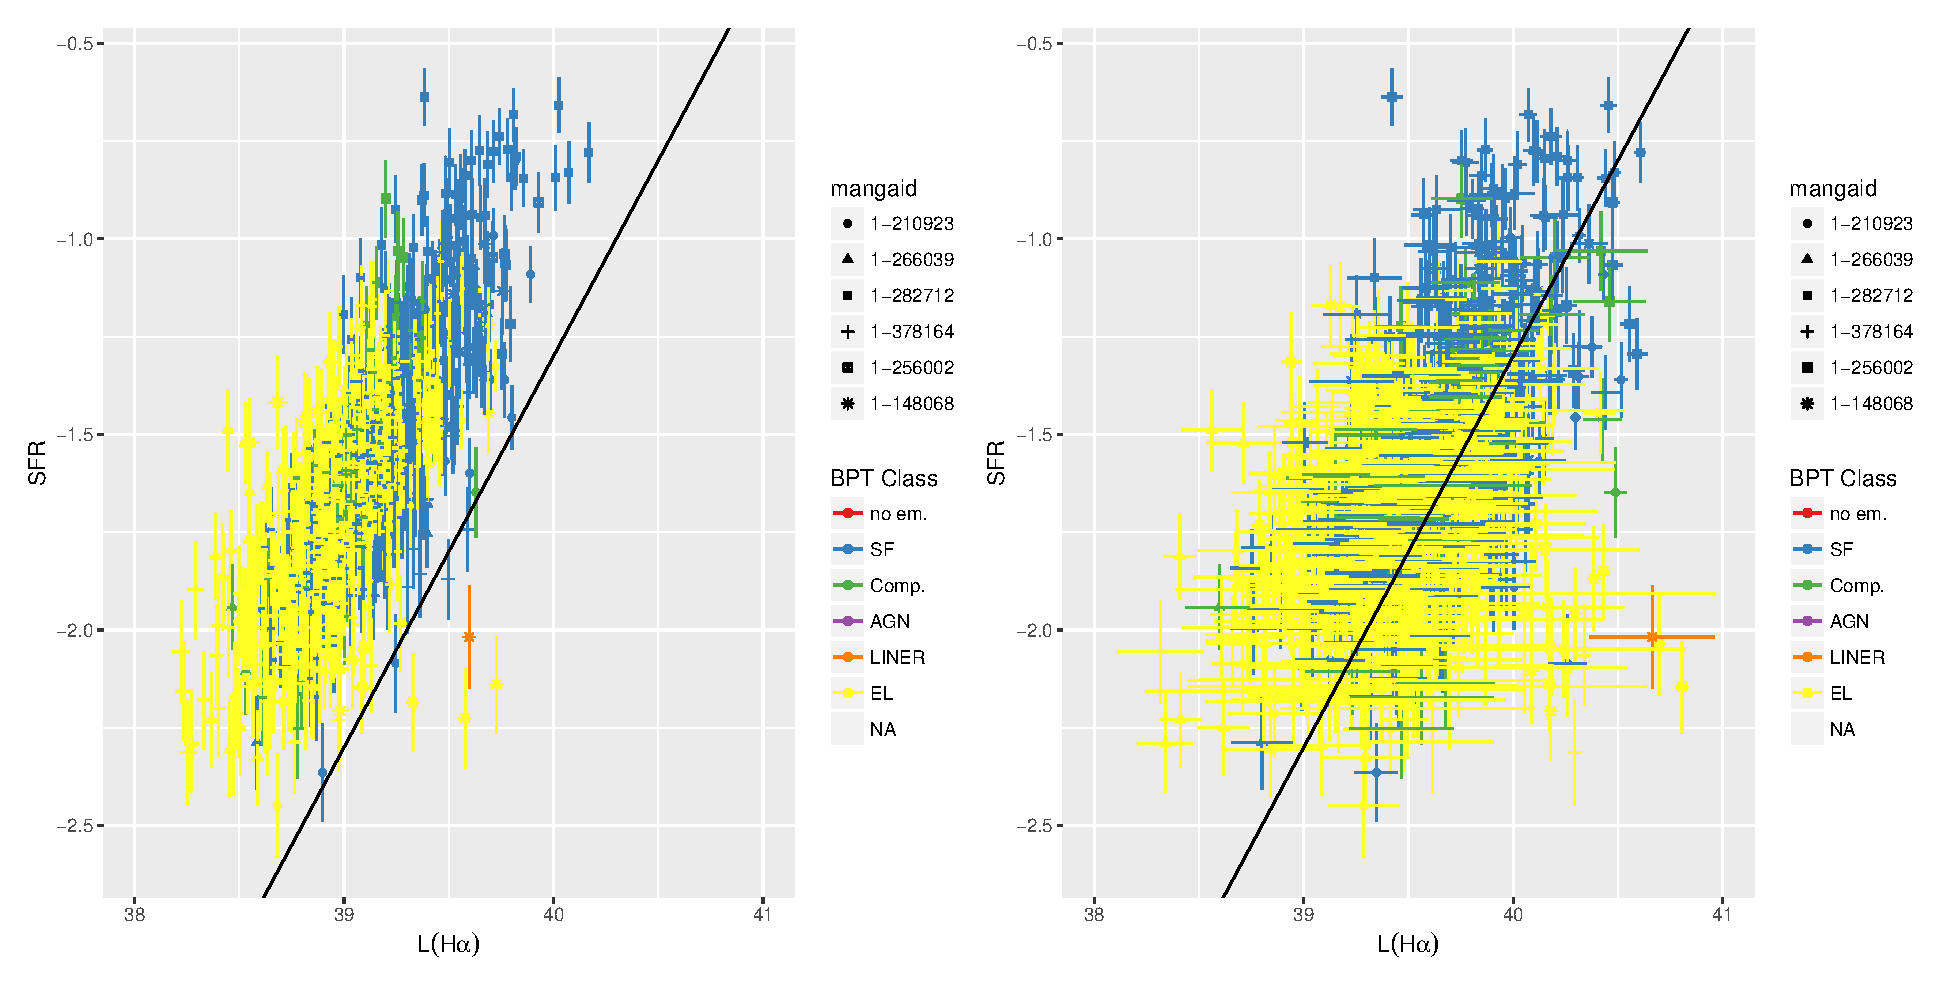
\includegraphics{sfrha.eps}}\hfill
\resizebox{0.25\textwidth}{!}{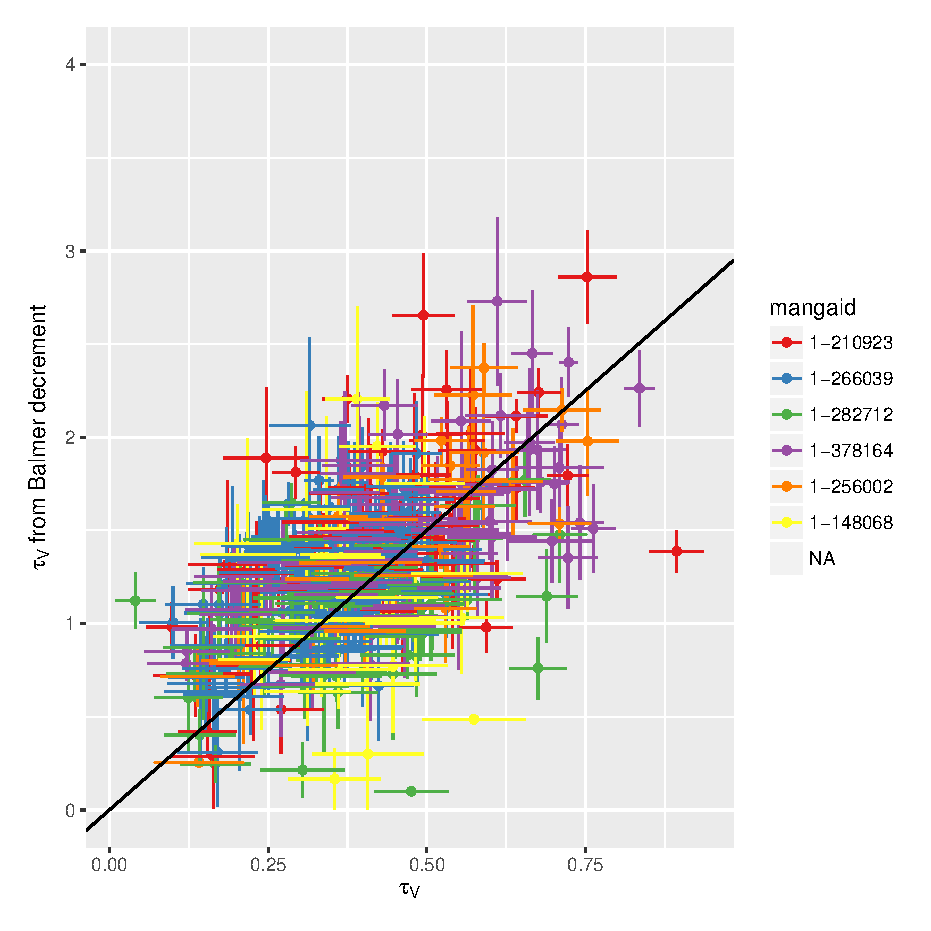
\includegraphics{tauvbd_tauv.eps}}
\caption{Modeled star formation rate vs. $H\alpha$ luminosity for all galaxies and all analyzed spectra. Left: $H\alpha$ luminosity uncorrected for internal attenuation. Middle: corrected using Balmer decrement with Calzetti attenuation relation. The straight line is the calibration of \citet{2006ApJ...642..775M} with a 0.2 dex shift to account for the difference in assumed IMFs \citep{2011ApJ...737...67M}. Right: Optical depth from Balmer decrement vs. optical depth from Stan models. Spectra with star forming line ratios only. Straight line has slope 3 \citep{2000ApJ...539..718C}.}
\label{fig:sfrha}
\end{figure*}

Turning to the results of the Stan models, figure \ref{fig:sfrha} plots the estimated log star formation rate (in M$_\sun$/yr.) against the log H$\alpha$ luminosity (in erg/sec.) for all analyzed spectra in the full sample. This includes spectra with non-starfroming line ratios -- many of the outliers in the lower right portion of the plot are from the nucleus and bar region of 1-148068. Plotted points are posterior means and the error bars are $\pm 1$ posterior standard deviations. In the left pane H$\alpha$ luminosity is uncorrected for internal attenuation. In the middle I use the observed Balmer decrement to correct for attenuation assuming an intrinsic H$\alpha$/H$\beta$ ratio of 2.86 and Calzetti attenuation. The straight line in both plots is the SFR-H$\alpha$ calibration of \citet{2006ApJ...642..775M} shifted by 0.2 dex to account for the different assumed IMFs \citep{2011ApJ...737...67M}. Although the scatter increases substantially because H$\beta$ is poorly constrained it's encouraging and somewhat surprising that modeled star formation rates are broadly consistent with the calibration over the $1 \frac{1}{2}$ order of magnitude range of estimates. Recall that the star formation rate is estimated as the average mass in stars born over 100 Myr and isn't directly affected by the emission line luminosity estimates, which in any case probe star formation over an at most 10 Myr time scale \citep{2012ARA&A..50..531K}.

The right pane of figure \ref{fig:sfrha} plots the optical depth estimated from the Balmer decrement against that estimated for the stellar component from the Stan models. For clarity only spectra with starforming emission line ratios are shown. The straight line has a slope of 3, consistent with the dust model of \citet{2000ApJ...539..718C} for starforming regions. This suggests that our attenuation model actually bears some resemblance to reality, while also hinting that a dual component dust model might be useful at least for starforming galaxies. What effect this would have on summary estimates such as stellar masses and star formation rates is hard to predict. Since the observed fluxes are well fit by the models over the whole wavelength baseline any reddened light from a young stellar population has been replaced with less reddened light from some mix of older populations in these fits -- in other words there is a dust-age ``degeneracy'' in addition to the many others that plague SED models.

\begin{figure*}
\resizebox{0.3\textwidth}{!}{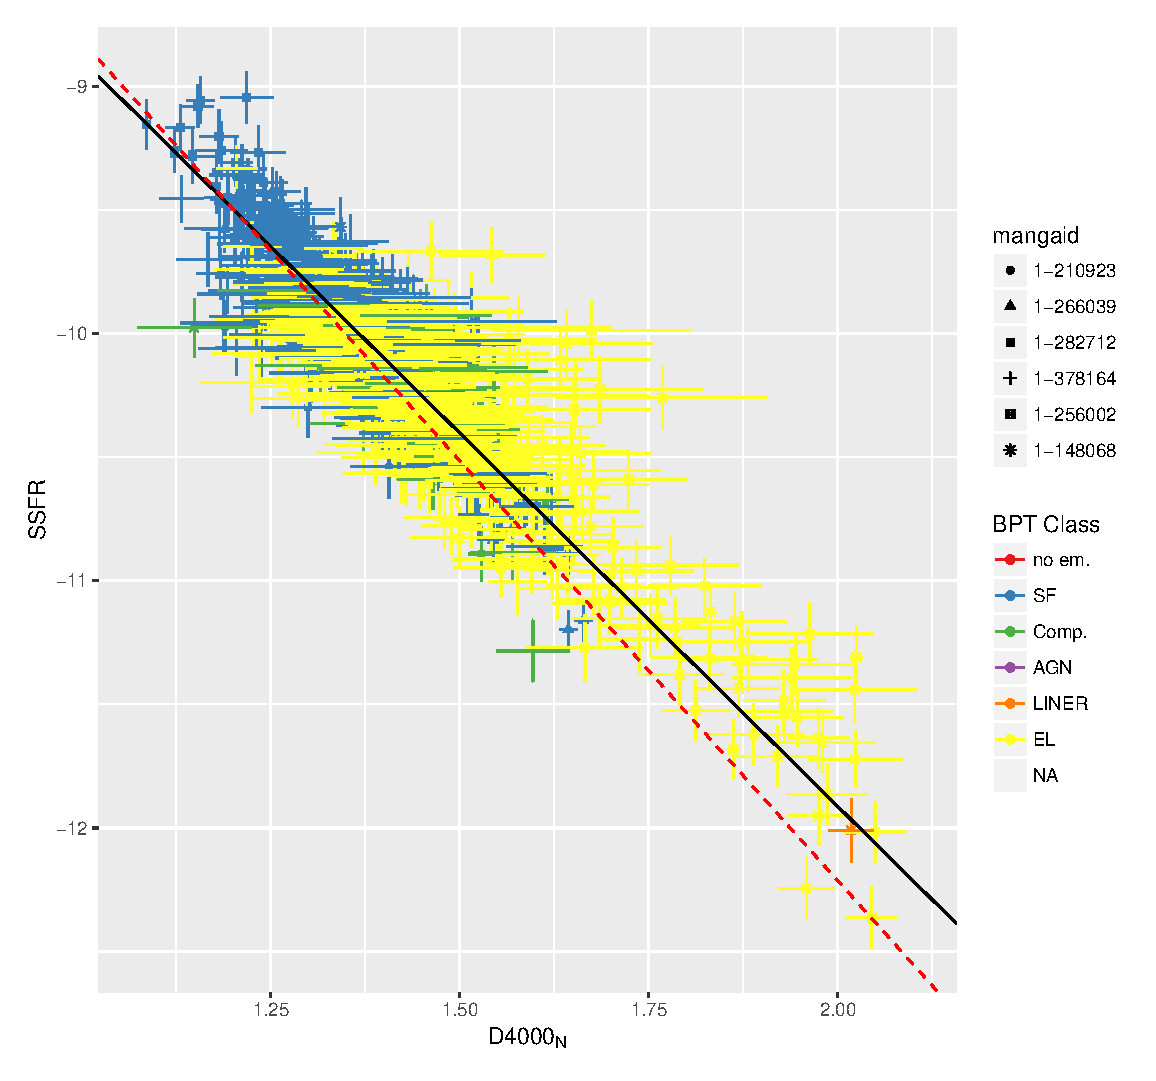
\includegraphics{ssfrd4000all.eps}}
\caption{Modeled \emph{specific} star formation rate ($yr^{-1}$) vs. $D4000_n$ for all galaxies and all analyzed spectra.}
\label{fig:ssfrd4000}
\end{figure*}

\citet{2004MNRAS.351.1151B} used D4000 to estimate specific star formation rates of SDSS galaxies with non starforming emission line ratios. The relationship between my measured values of D$4000_n$ and modeled SSFR is shown for all analyzed spectra in the full sample in figure \ref{fig:ssfrd4000}. The black straight line is a simple Bayesian errors in variables fit to the data taking into account the estimated uncertainties. I was unable to find a quantitative calibration of the relationship in the literature, but Figure 11 of \citet{2004MNRAS.351.1151B} is qualitatively similar to figure \ref{fig:ssfrd4000}. The red dashed line is a fit using the same errors in variables model to a sample of $\approx 22000$ SDSS legacy galaxy spectra from a region around the north galactic pole with fiber SSFR estimates and D$4000_n$ measurements retrieved from the MPA-JHU analysis through SDSS CasJobs\footnote{\url{http://skyserver.sdss.org/CasJobs/}. The MPA-JHU analysis pipeline was last applied to the DR8 spectroscopic sample \citep{2011ApJS..193...29A}.}. The agreement is very close, which again is encouraging and a bit puzzling. \citet{2004MNRAS.351.1151B} don't clearly state over how long a period of time their SSFR estimate is averaged. They claim that the calibration is based on spectra with starforming line ratios with the resulting SFR/M$_\star$--D4000 relationship applied to the remainder of the sample, but they don't explain how the calibration was extended to SSFR values as low as $\sim 10^{-12}$, which by any measure is passively evolving. Star formation rates for spectra with starforming line ratios were based on emission line fluxes which would imply a timescale of $\sim 10^7$ years, an order of magnitude shorter than my SSFR estimates. Mine are based solely on the SSP model fits to a much longer wavelength baseline than the 4000\AA~ break region, which makes the tightness of the relationship another surprise.

In any case given the encouraging agreement between my model estimates of star formation rates and independent calibrations I concentrate on these for the remainder of this section, along with mass growth histories.

\begin{figure*}[ht]
\centering
\resizebox{\textwidth}{!}{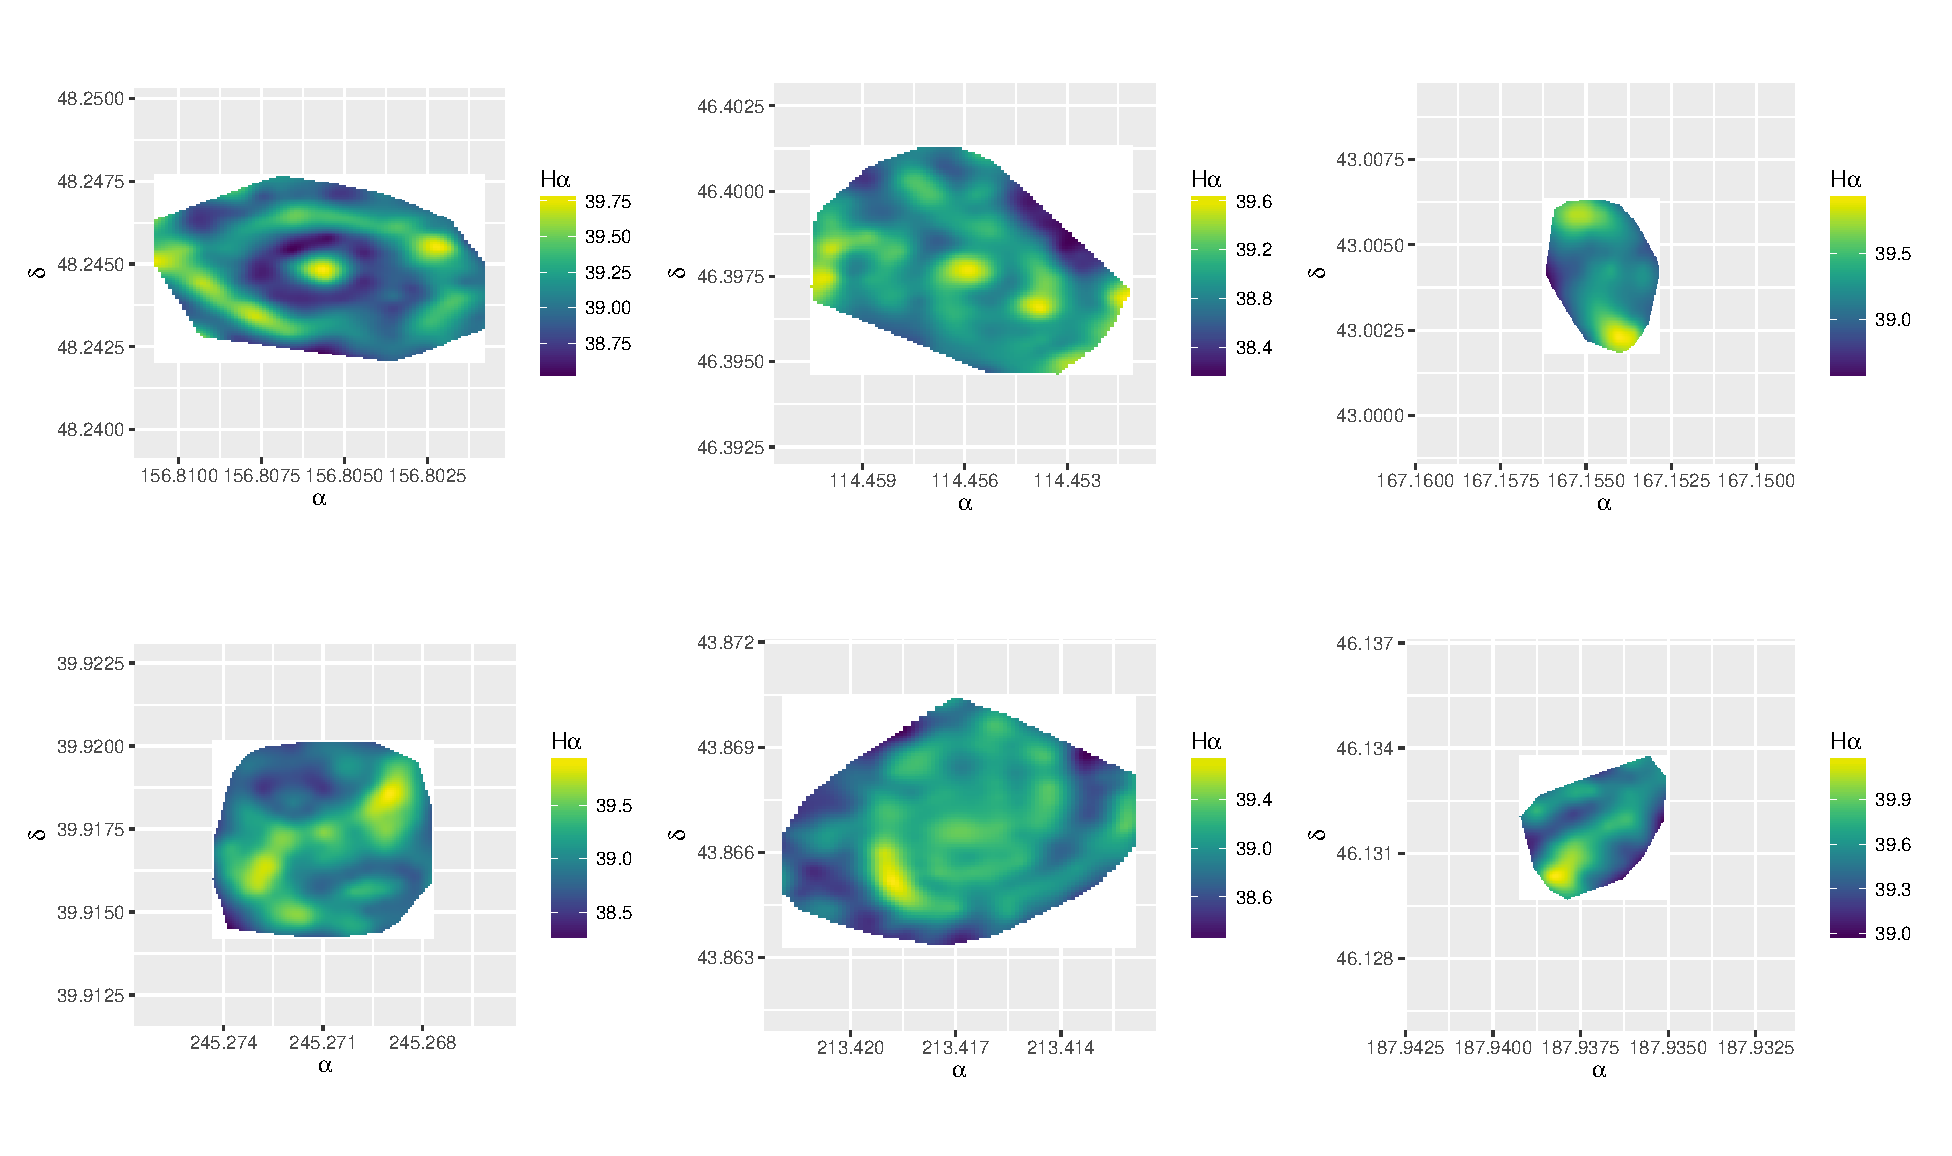
\includegraphics{halphamaps.eps}}
\caption{H$\alpha$ luminosity in erg/s., uncorrected for internal attenuation.}
\label{fig:halphamaps}
\end{figure*}

\begin{figure*}[hb]
\centering
\resizebox{\textwidth}{!}{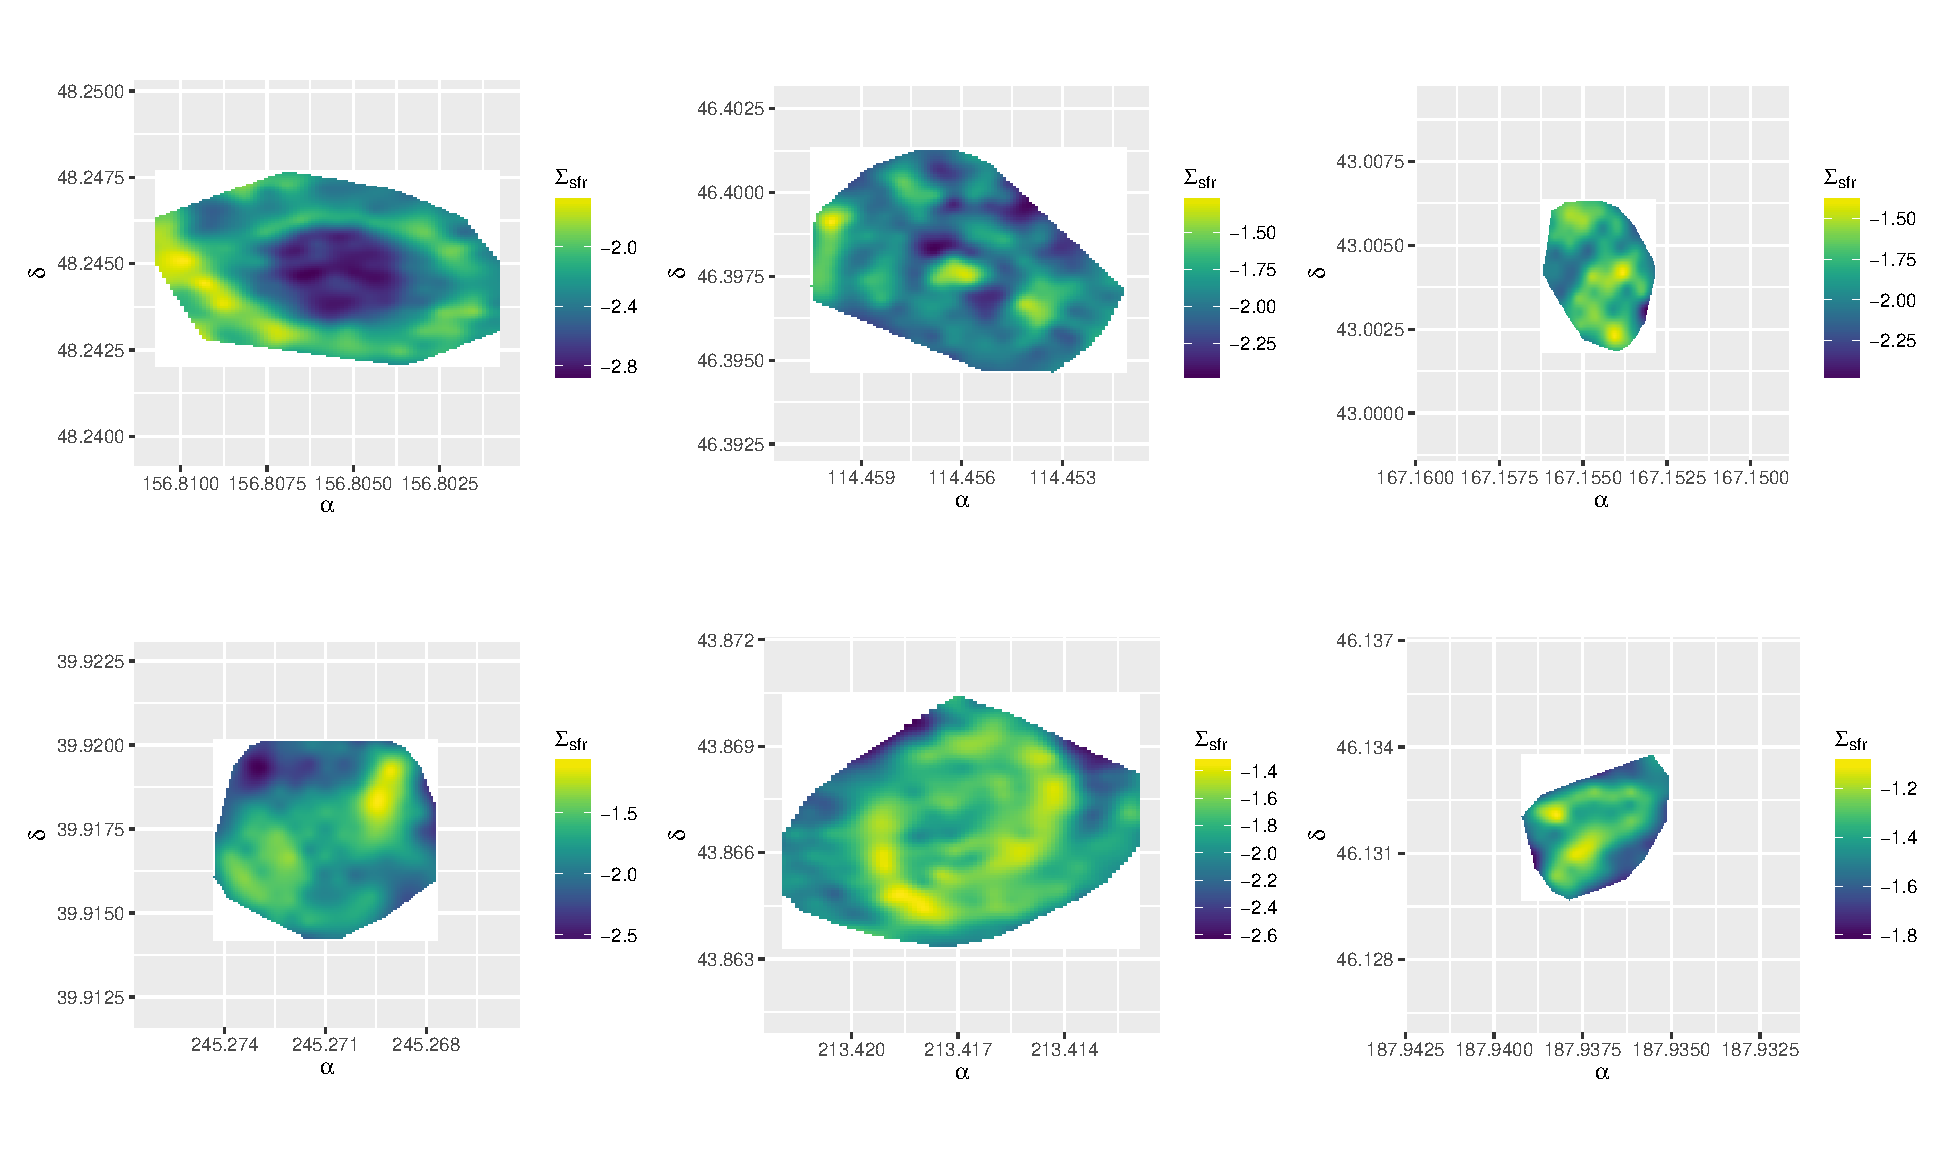
\includegraphics{sigmasfrmaps.eps}}
\caption{Modeled star formation rate density ($M_\sun/yr/kpc^2$).}
\label{fig:sigmasfrmaps}
\end{figure*}

Figure \ref{fig:halphamaps} plots maps of log H$\alpha$ luminosity in erg/s, uncorrected for internal attenuation. Maps of SFR surface density in M$_\sun$/yr/kpc$^2$ and SSFR in yr$^{-1}$ are in figures \ref{fig:sigmasfrmaps} and \ref{fig:ssfrmaps}. Not surprisingly areas of high SFR density closely track areas of high H$\alpha$ luminosity and nicely outline the spiral arms in most of the sample. The red galaxy 1-256002 has an interesting morphological peculiarity of a bar and outer ring or pseudo ring with what appear to be very short spiral arms extending from the intersection of the bar with the ring. Those are seen to be large HII regions with active star formation in the maps.

\begin{figure*}[ht]
\centering
\resizebox{\textwidth}{!}{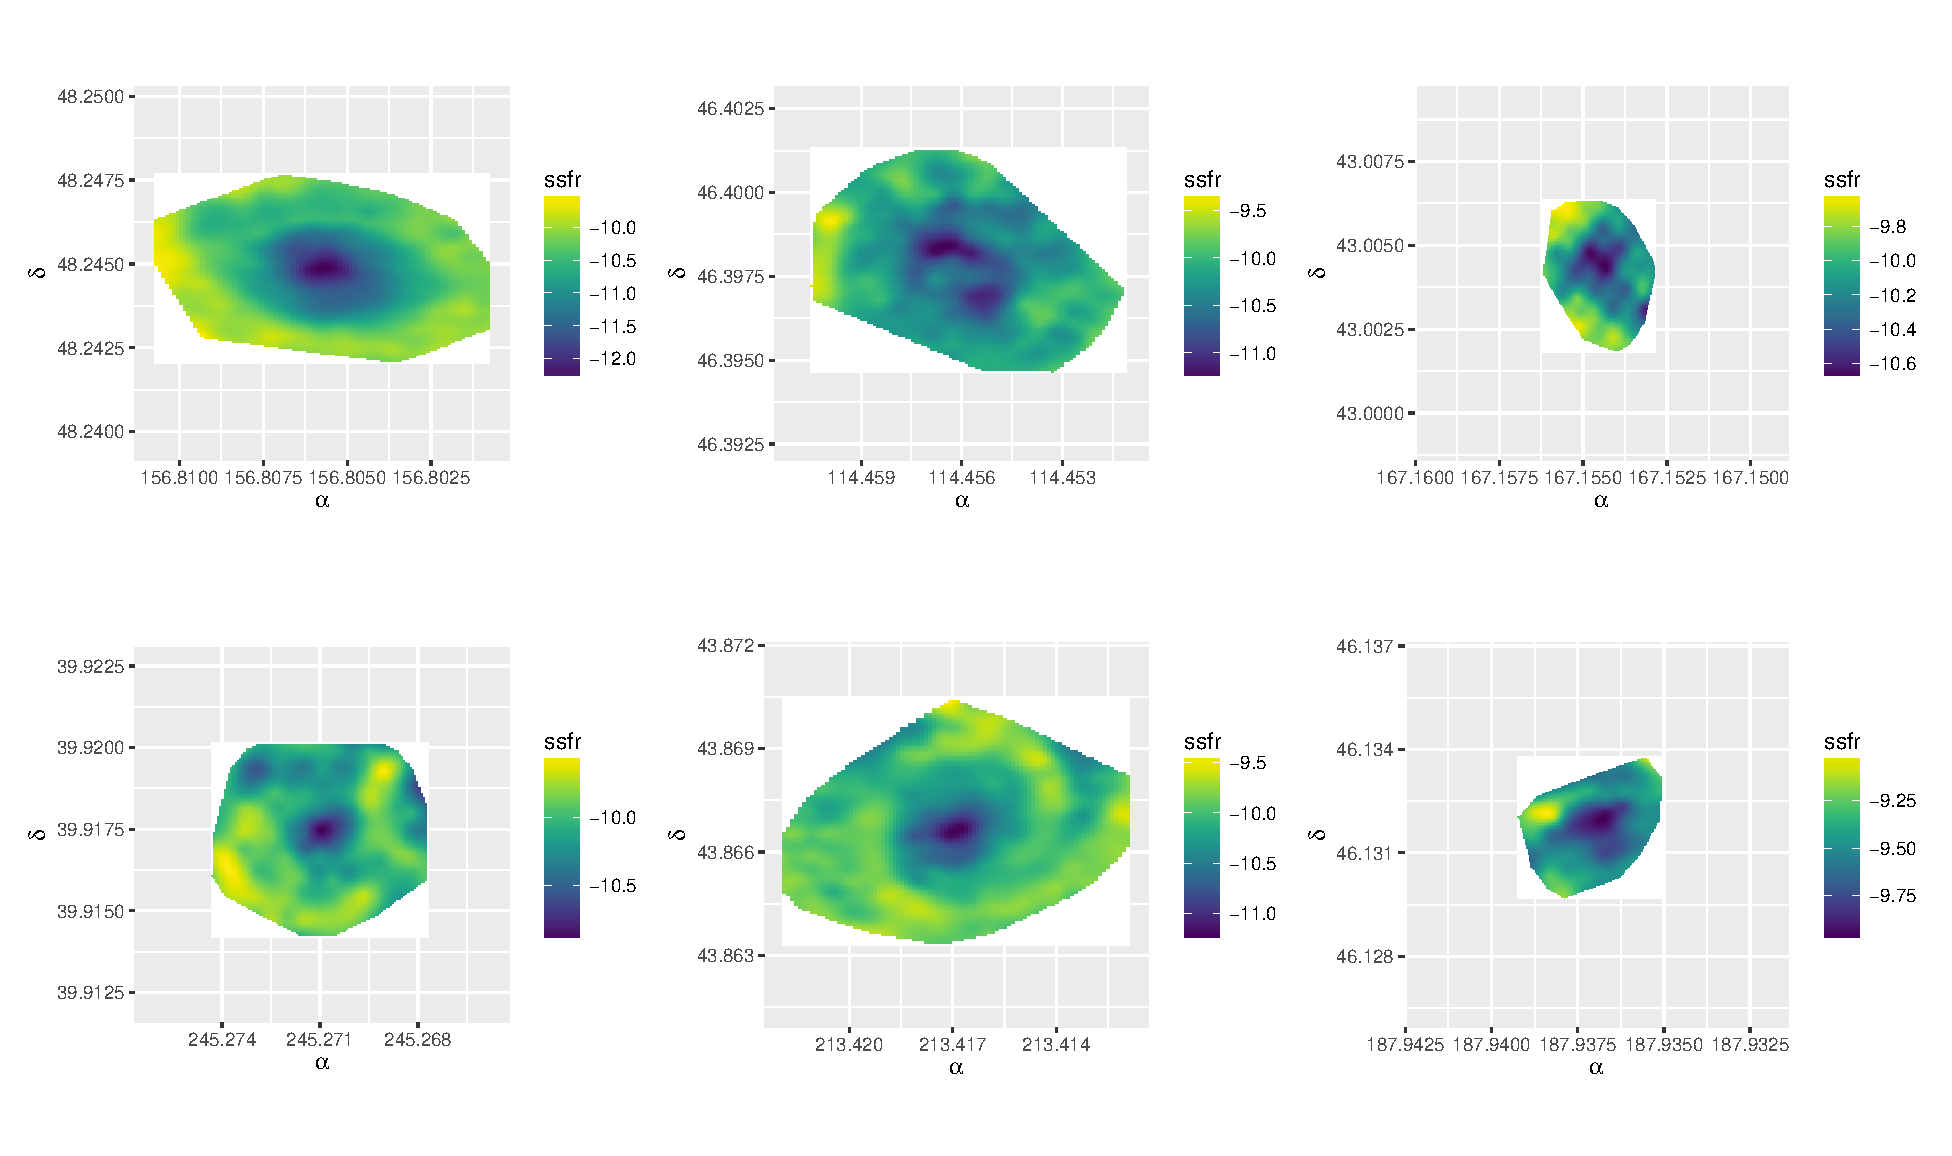
\includegraphics{ssfrmaps.eps}}
\caption{Modeled specific star formation rate ($yr^{-1}$).}
\label{fig:ssfrmaps}
\end{figure*}

That the red sample galaxy 1-148068 has a central AGN is clearly indicated by its combination of high central H$\alpha$ luminosity and complete absence of star formation in the inner $\approx 4$kpc. The central region of the blue spiral 1-210923 is also somewhat overluminous in H$\alpha$ compared to its central SFR density and its emission line ratios put it in the composite region of the BPT diagram, which makes it possibly the only true AGN/SF composite in this sample. All other galaxies in the sample have some detectable level of central star formation.

\begin{figure*}[ht]
\resizebox{\textwidth}{!}{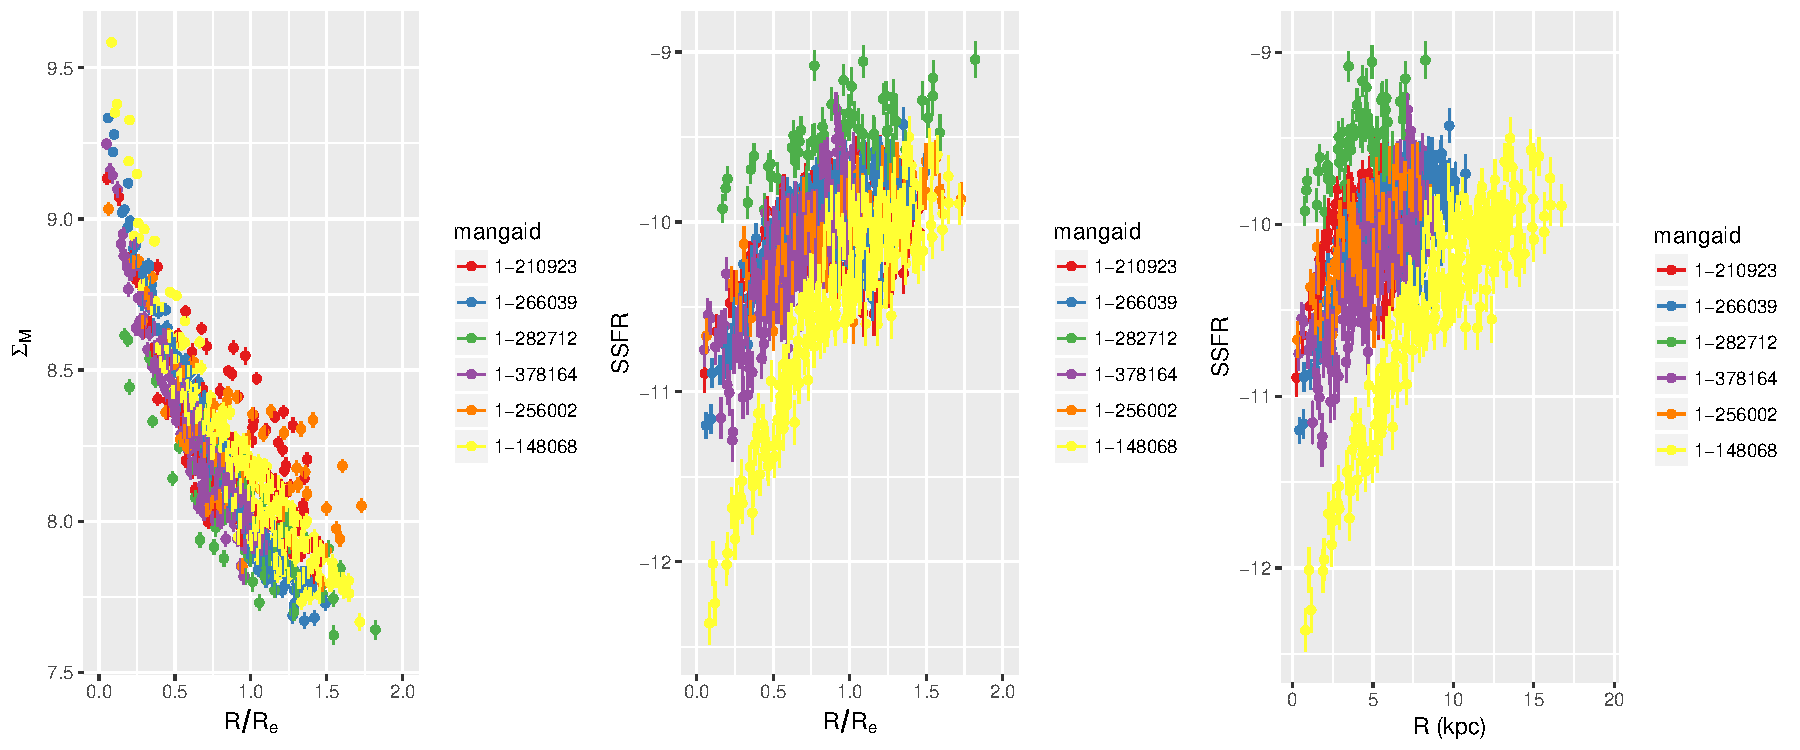
\includegraphics{mstarssfrre.pdf}}
\caption{Left: log stellar mass density (M$_\sun$/kpc$^2$) vs. projected radius in effective radii. Middle: specific star formation rate ($yr^{-1}$) vs. projected radius. Right: specific star formation rate vs. project radius in kpc. Values are for all analyzed spectra in all sample galaxies. Error bars are $\pm 1 \sigma$ credible intervals.}
\label{fig:mstarssfr}
\end{figure*}

Regions of high \emph{specific} star formation rate are more diffusely distributed than regions of high star formation rate density, and SSFR anti-correlates with mass density. This can be seen in figure \ref{fig:mstarssfr} which plots, on the left, the run of stellar mass density against projected distance from the IFU center (assumed to correspond to the system center) relative to r band effective radii, and in the right two panes SSFR against projected distance in effective radii and kpc. All of the mass profiles are exponential, with some having a steeper inner profile indicating the presence of a bulge or pseudo bulge \citep{1970ApJ...160..811F, 2006A&A...454..759P, 2008ApJ...683L.103B}. Specific star formation rates \emph{increase} exponentially with radius, with some signs of turnover at large radii. 

\begin{figure*}[ht]
\resizebox{0.3\textwidth}{!}{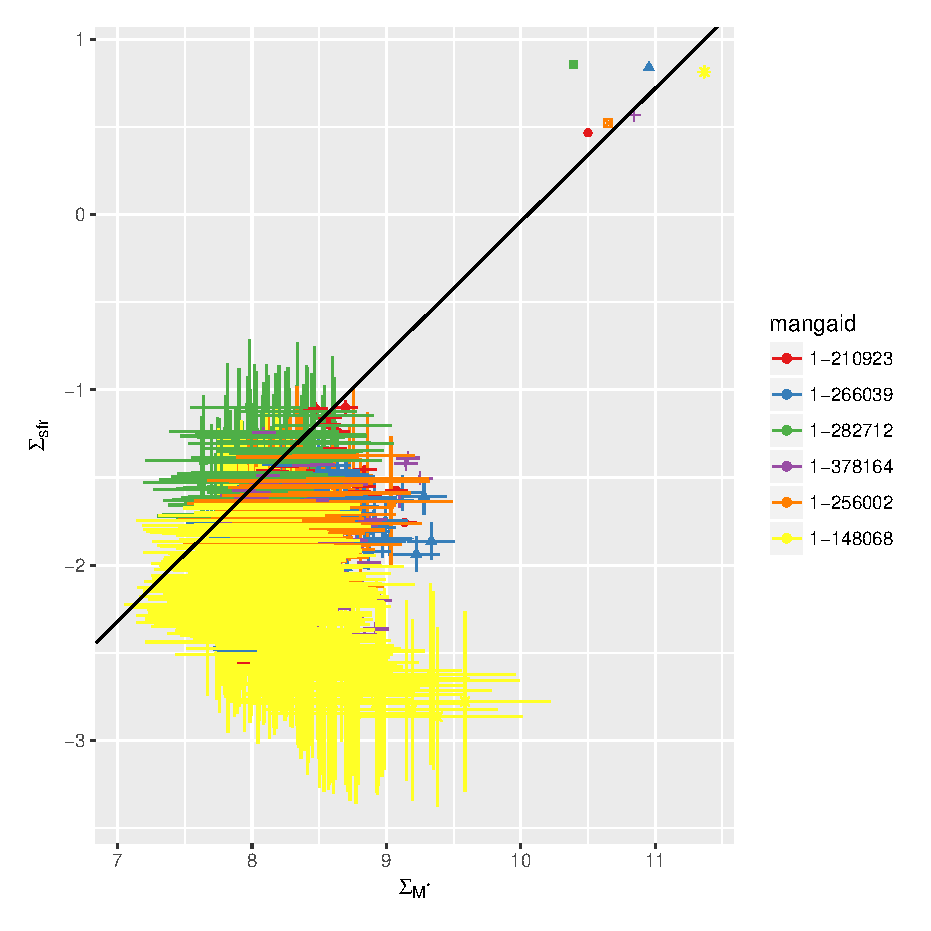
\includegraphics{sfrmstar.eps}}
\caption{Star formation rate density ($M_\sun/yr/kpc^2$) vs. stellar mass density ($M_\sun/kpc^2$)for all galaxies. The points at upper right are total masses and star formation rates. These were calculated by summing all analyzed spectra, with no further extrapolation.}
\label{fig:sigmasfrsigmamstar}
\end{figure*}

Figure \ref{fig:sigmasfrsigmamstar} plots the log of the star formation rate density in M$_\sun$/yr/kpc$^2$ against log stellar mass density in M$_\sun$/kpc$^2$ for all analyzed spectra, color coded by galaxy. For reference the straight line gives the estimated mean starforming main sequence relation of \citet{2015ApJ...801L..29R}. My SFR-M$_\star$ estimates scatter broadly around the main sequence with a long tail of quiescently or passively evolving regions. At the upper right of the plots are estimated total stellar masses and star formation rates created by summing the estimates for each spectrum (again with no attempt to extrapolate). All of the galaxies cluster around the main sequence with a scatter that's consistent with cosmic variance. Although I caution against generalizing from this small sample this is consistent with the main claim of \citetalias{2012A&A...543A.132C} that red sample galaxies are forming stars at normal rates for their masses.

\begin{figure*}
\centering
\resizebox{0.3\textwidth}{!}{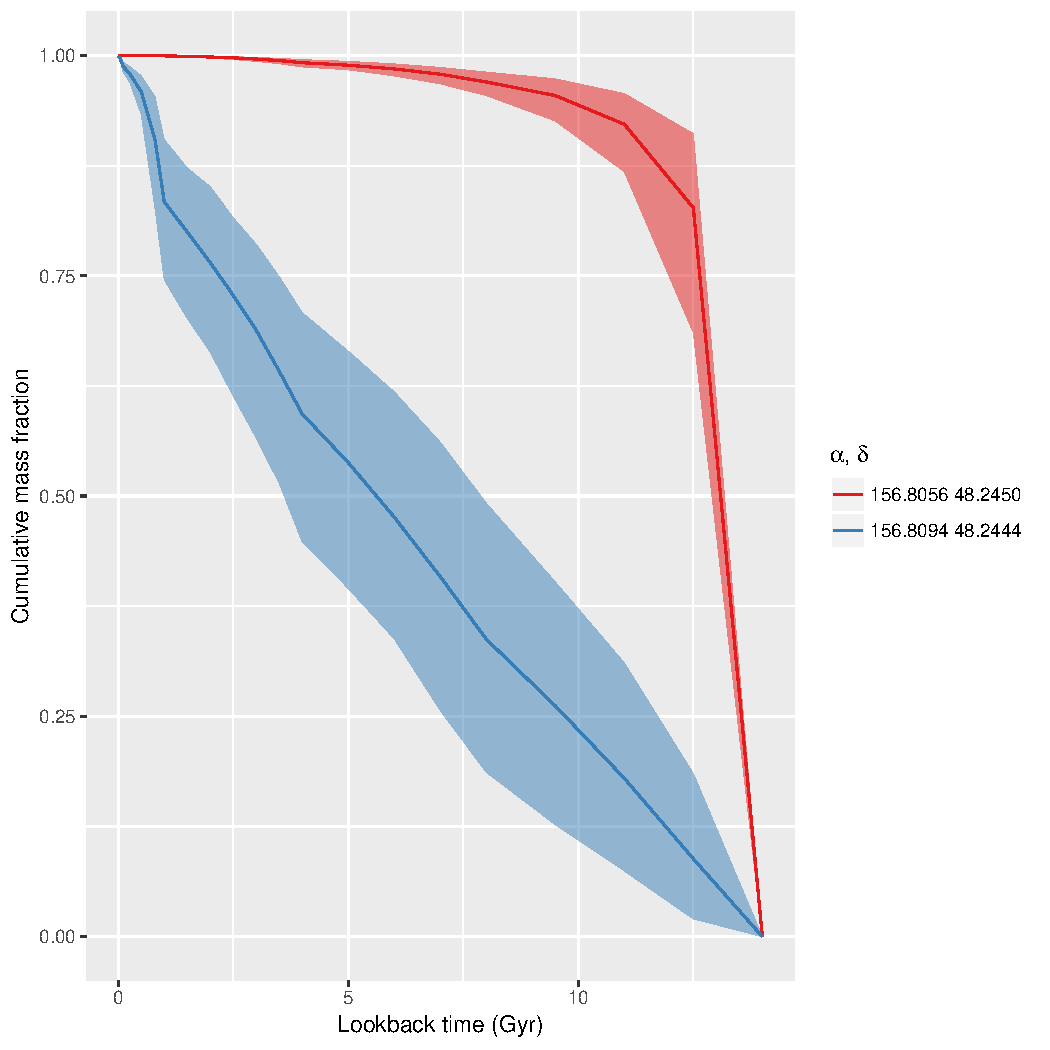
\includegraphics{mgh2_1_14.pdf}}\hfill
\resizebox{0.3\textwidth}{!}{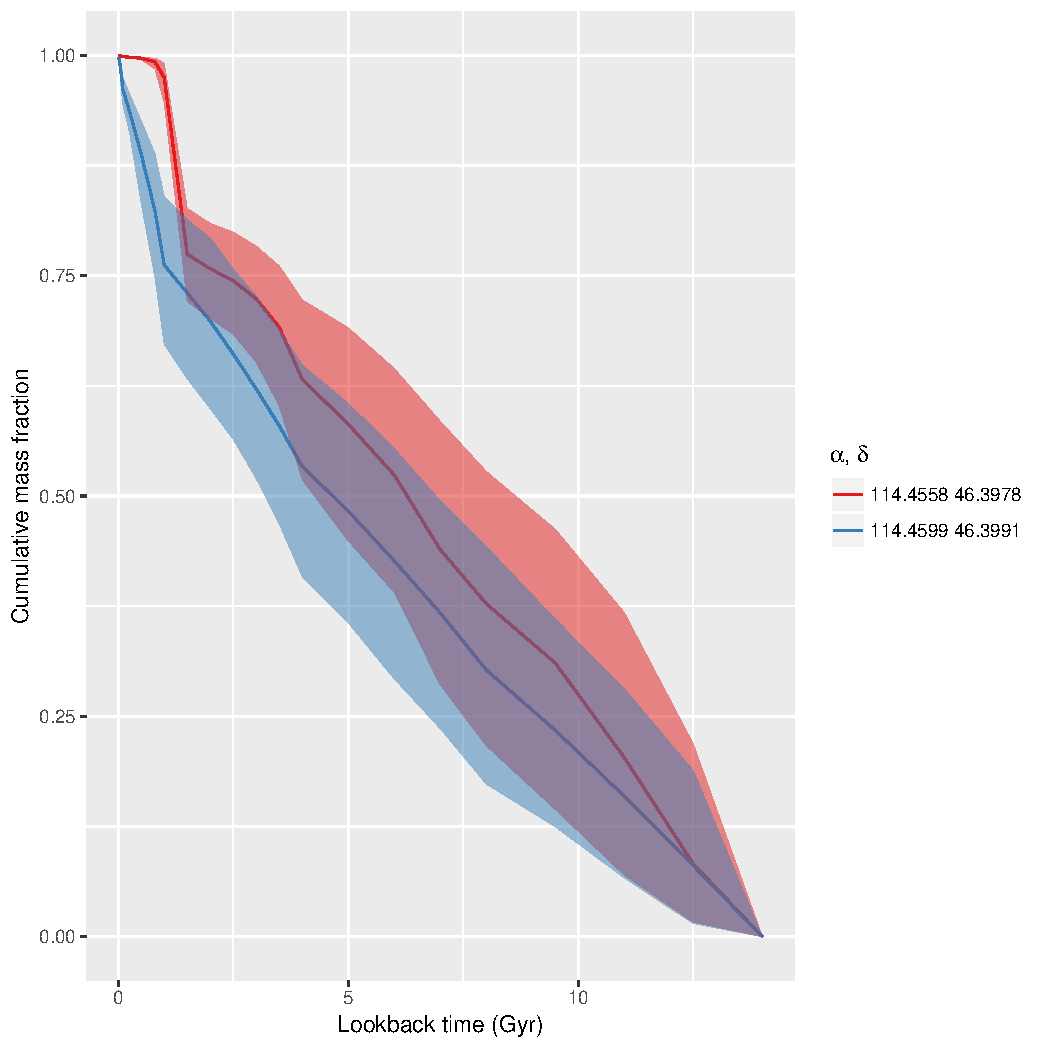
\includegraphics{mgh2_1_37.pdf}}\hfill
\resizebox{0.3\textwidth}{!}{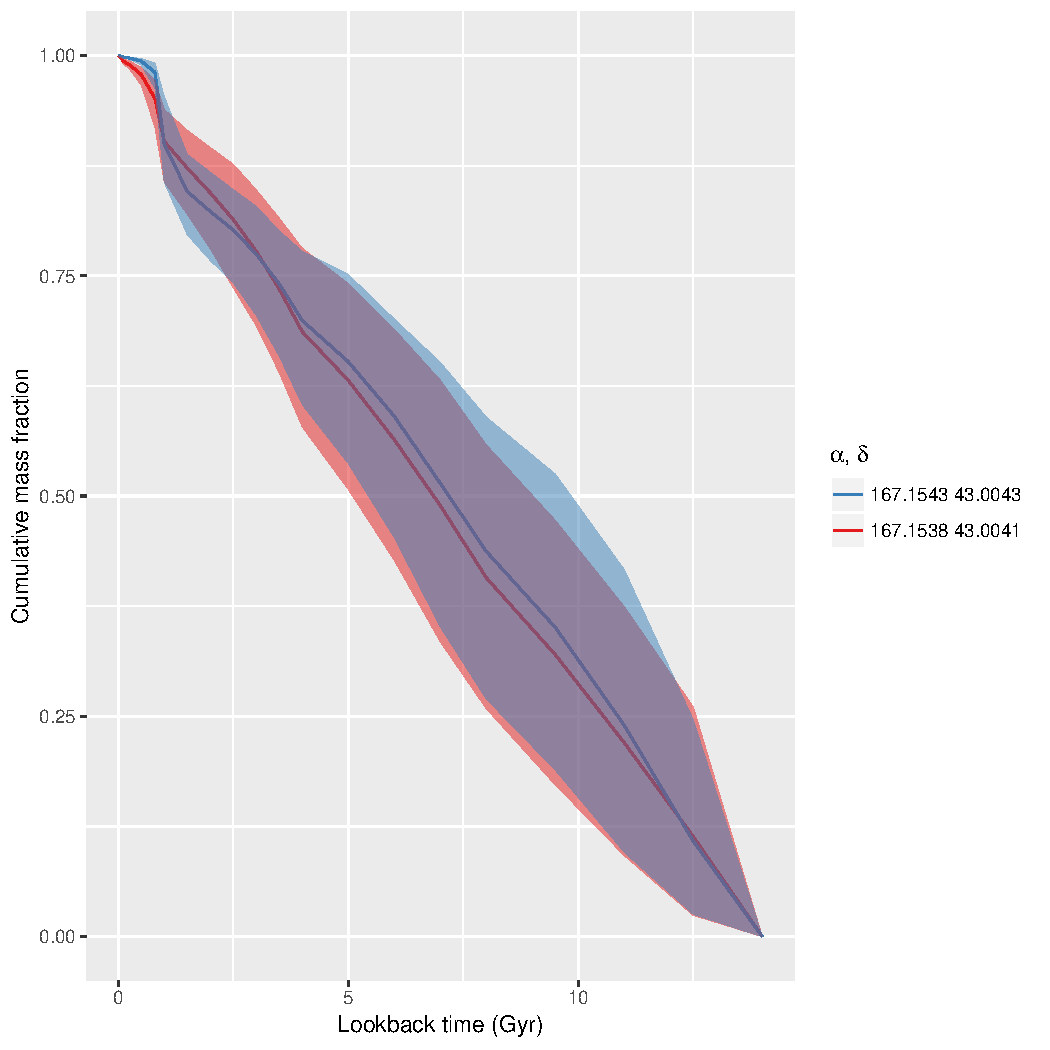
\includegraphics{mgh2_1_25.pdf}}\vfill
\resizebox{0.3\textwidth}{!}{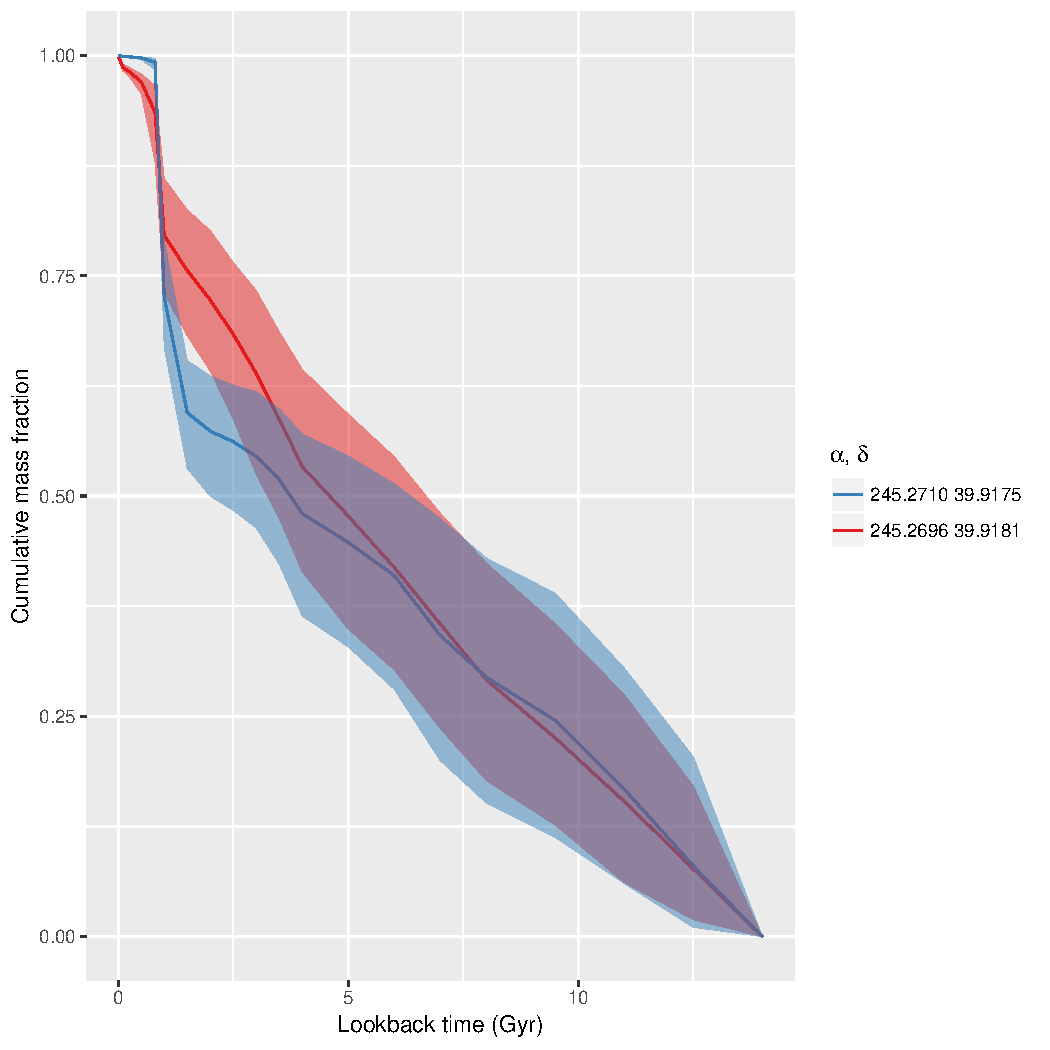
\includegraphics{mgh2_1_21.pdf}}\hfill
\resizebox{0.3\textwidth}{!}{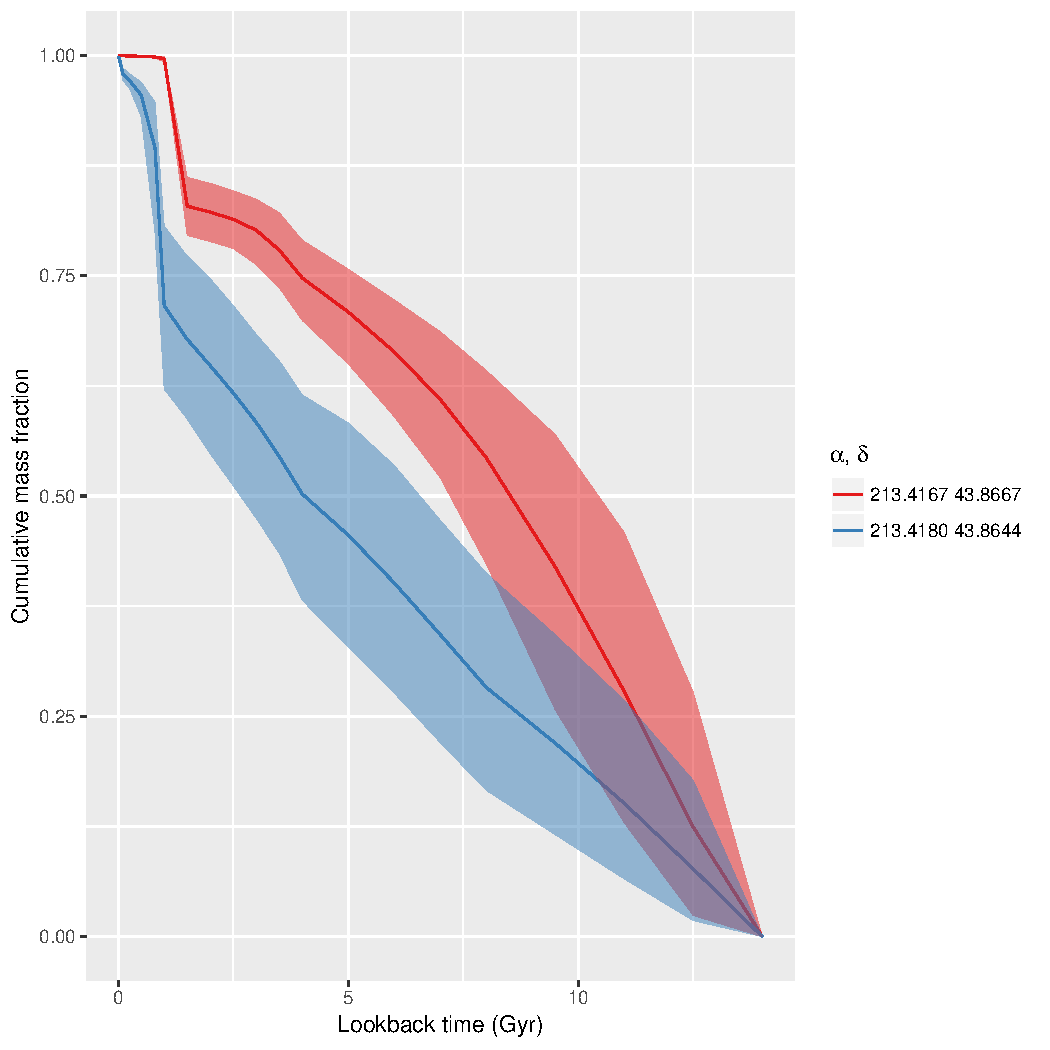
\includegraphics{mgh2_1_26.pdf}}\hfill
\resizebox{0.3\textwidth}{!}{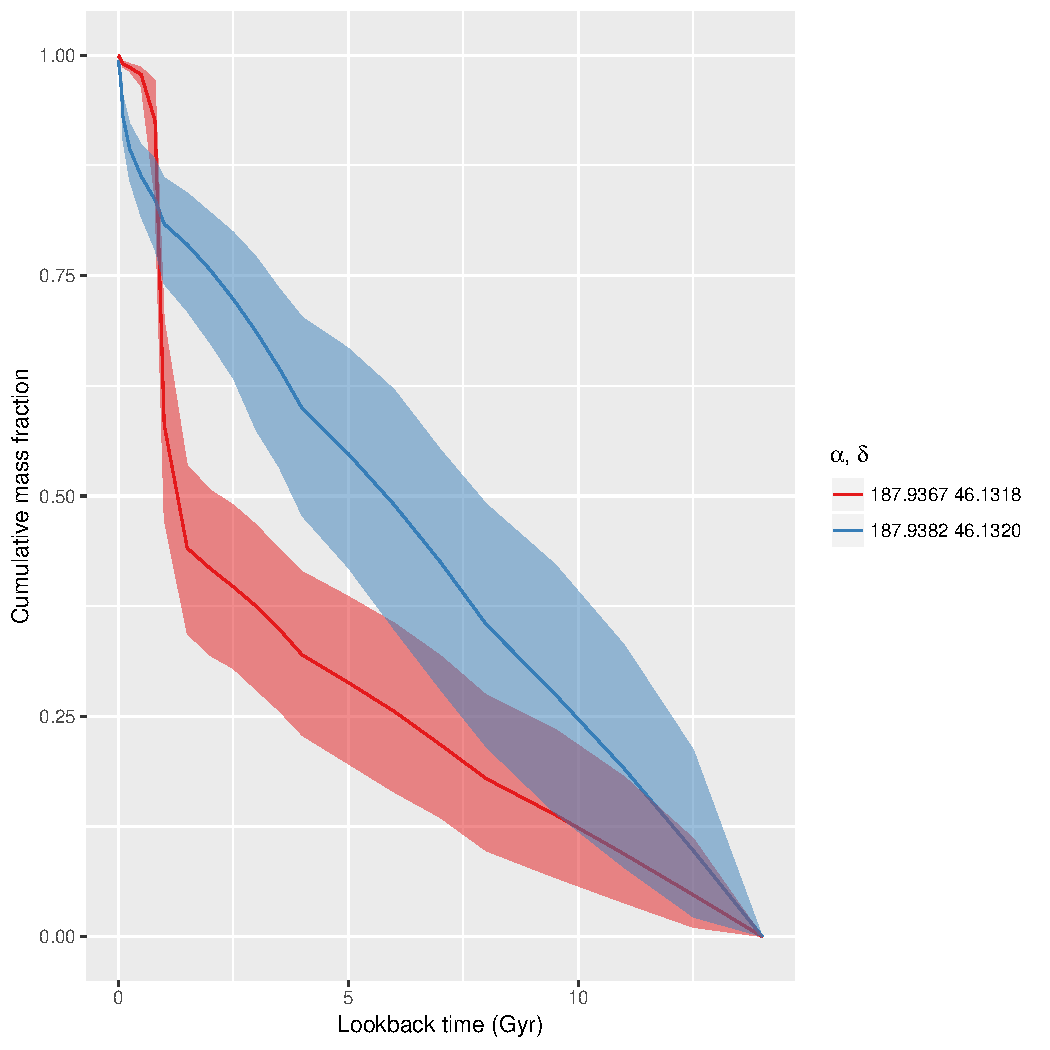
\includegraphics{mgh2_1_28.pdf}}

\caption{Mass growth histories in the central fiber and the fiber with highest mean star formation rate density in each galaxy. Lines are posterior mean values, with symmetrical 95\% confidence intervals plotted as translucent bands.}
\label{fig:twomgh}
\end{figure*}

Figure \ref{fig:twomgh} shows a sample of estimated mass growth histories for all galaxies. For clarity I show estimates for the central fiber and the one with highest current star formation rate only. This choice was unilluminating for the red spiral galaxy 1-256002 where the highest star formation rate density is in a fiber adjacent to the central fiber and mass growth histories are nearly identical. There is a clear pattern of inside-out mass assembly \citep{2013ApJ...764L...1P, 2016A&A...590A..44G} in most of the sample, and this is especially evident in the red galaxy 1-148068 which had as much as $\approx 95\%$ of its present day stellar mass in place by 10Gyr ago ($z \sim 2$) and is currently passively evolving in the central several kpc. 

The blue sample galaxy 1-282712 appears to be an exception, but this is something of an artifact of displaying relative rather than absolute mass growth. What appears to have happened if the model star formation histories are to be believed is there was a centrally concentrated acceleration of star formation that began $\approx 1$Gyr before the light left the galaxy that subsequently spread outward, with the galaxy now experiencing a global starburst. This hints at a possible recent encounter with a fresh source of fuel although no morphological disturbance or near neighbors are noted.

Many of the mass growth histories show a substantial fraction -- anywhere from 10 to nearly 50\% -- of the present day stellar mass is in intermediate ($\lesssim 1.5$Gyr) age stars. This was already anticipated by figure \ref{fig:d4000hd} which shows that a large fraction (30\%) of the analyzed spectra have H$\delta_A$ EW$> 5$\AA, which is a commonly adopted threshold for H$\delta$ strong galaxy selections \citep{2003PASJ...55..771G}. There are several possible interpretations of this, and it should be kept in mind too that the very presence of an intermediate age population obscures the earlier star formation history and most likely (per section \ref{sec:mocks}) biases the mass contribution of older populations downwards. First, since star formation is spatially localized it might be unsurprising that regions of the disk outside the most active starforming areas have a large intermediate age population. Alternately, star formation could be ongoing but hidden, a common interpretation of galaxies with large Balmer equivalent widths and significant emission \citep{1999ApJ...518..576P}. As already mentioned a highly reddened young population might be masquerading as a slightly older and less reddened one given the single component dust model used here. Other ingredients could be missing from the SSP models as well: \citet{2010ApJ...709...88O} showed that blue horizontal branch stars can masquerade as a late time burst, although this was only found to be an issue in rather metal poor globular clusters. These galaxies all have approximately solar metallicity and there's no evidence for a significant metal poor population in any.

\begin{figure*}
\resizebox{0.5\textwidth}{!}{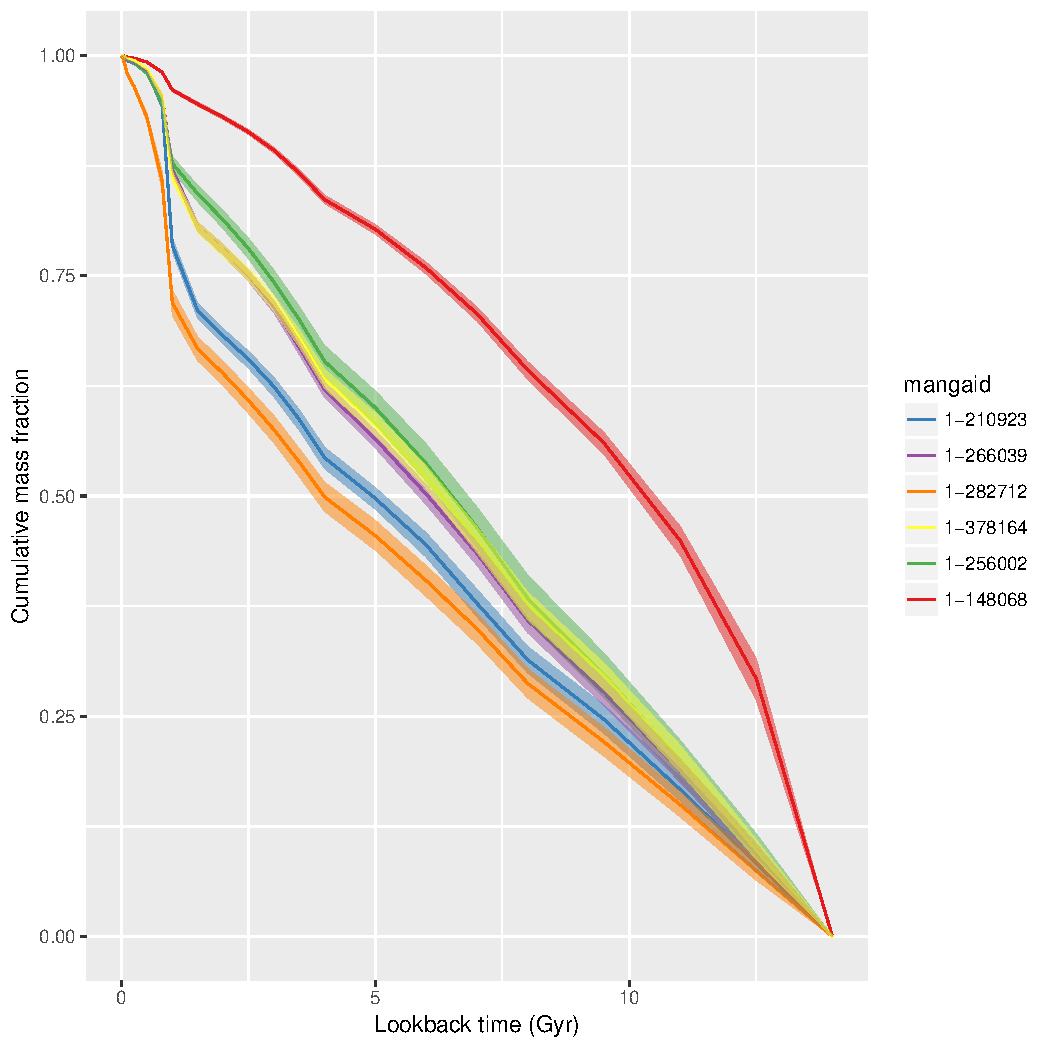
\includegraphics{mgh_all.pdf}}
\caption{Summed mass growth histories for all galaxies in the sample.}
\label{fig:totalmgh}
\end{figure*}

Finally, figure \ref{fig:totalmgh} shows summed mass growth histories for the full sample. Again the red spiral 1-148068 stands out for reaching any given percentage of its current stellar mass at an earlier age than any of the rest of the sample. The remaining galaxies all show some global late time acceleration of star formation. Whether this represents a real rejuvenation or is an artifact of priors or peculiarity of the SSP models requires further investigation.

Both bars and active galactic nuclei are thought to play a role in regulating star formation, but while the theoretical picture is reasonably clear \citep{2004ARA&A..42..603K, 2013seg..book....1K, 2013ARA&A..51..511K} the observational situation is less so, particularly with respect to bars \citep{2012ApJS..198....4O}. At least three of the galaxies in this sample have bars. A fourth, 1-210923, is classified by \citet{2010ApJS..186..427N} as T type 5 with an intermediate strength bar, which was mapped to Sc (not SBc) in NED. On the other hand it received a weighted vote fraction for the presence of a bar of 0.91 in Galaxy Zoo 2 \citep{2013MNRAS.435.2835W}, the same as its counterpart 1-148068 in the red sample. Also note the twisted inner isovelocity contours in figure \ref{fig:vfs} that indicate streaming motions along the inner arms, a bar-like kinematic feature. Among these 4 there is a diverse range of star formation histories both globally and in central regions. Only 1-148068 shows unambiguous evidence for an AGN, and it's the only galaxy in this sample with strongly suppressed central star formation. Whether this predicts anything about red late type galaxies in general remains to be seen.

\section{CONCLUSIONS}
\label{sec:end}

The main technical result of this investigation is summed up succinctly in figure \ref{fig:traceplots}. The version of the Hamiltonian Monte Carlo sampling algorithm implemented in Stan adapts rapidly, with parameter samples converging to stationary distributions within a vary short warmup period and efficient exploration of the posterior thereafter. Modeled star formation histories vary continuously in distribution and appear to be consistent with other astrophysical constraints, as do summary estimates of physical properties.

This may be unique to Stan, or at least to HMC sampling. At present there are two reasonably mature implementations of HMC/NUTS available to the public, the other one being PyMC3\footnote{\url{https://github.com/pymc-devs/pymc3}} \citep{10.7717/peerj-cs.55}, a Python package that also implements a number of other MCMC and Gibbs samplers. There is relatively little comparative performance information available at present and its suitability for this task is completely unknown, but it may be an attractive alternative especially for users of the Python version of \texttt{ppxf}.

The mock spectrum simulations reported in \ref{sec:mocks} showed that systematic uncertainties dominate random ones, especially in objects with unusual star formation histories. The role of the prior in this still needs investigation. Preliminary experiments indicate that using priors that respect astrophysical constraints may considerably reduce biases. It's likely though that systematics will always be important given the daunting list of ``known unknowns'' \citep{2013ARA&A..51..393C} that are difficult to model.

There are several model extensions that are desirable or at least worth considering. Incorporating kinematics into the model is a priority (see appendix \ref{sec:kinstan} for some very preliminary work). Other straightforward possible additions include power law continuum emission which would require adding just two parameters (an amplitude and spectral index) or a more flexible prescription for attenuation. A possible way to constrain the contribution of poorly understood phases of stellar evolution such as the blue horizontal branch or ``thermally pulsing AGB" \citep[TP-AGB,][]{2005MNRAS.362..799M} stars would be to add subpopulations to the library of SSP models. This would allow direct estimates of their potential contributions or at the least expose additional degeneracies.

\appendix
\section{Stan code}
\label{sec:code}

This appendix lists the Stan code for the models discussed in this paper. Source files are included with the original \LaTeX~manuscript or provided on request to the author.

\lstinputlisting{spm_dust_em.stan}

\section{Kinematic modeling in Stan}
\label{sec:kinstan}

This section describes some very preliminary efforts to incorporate kinematics into Stan models. This is a partially parametric approach, with the stellar LOSVD estimated non-parametrically as a convolution kernel while gas kinematics are estimated parametrically. As with the pure SED modeling code in the previous section the source is included with the original \LaTeX~manuscript. The code is likely to change, perhaps radically, in future versions.

Since the code is more complicated some commentary may be helpful. The current version (2.16.2 at the time of writing) of Stan has no support for FFTs and specifically not convolution by FFT, so convolution is done by direct multiplication and summation of the SSP spectra with a convolution kernel of fixed length (at runtime of the Stan model). The kernel is declared as a simplex -- a K simplex being a vector of length K of nonnegative real numbers that sum to 1 (hence each element is $\le 1$).

The velocity distributions in emission lines are estimated parametrically using the same idea discussed in the text of treating them as conceptual delta functions which are trivially convolved with the gas LOSVD, for which I use the now standard Gauss-Hermite polynomial expansion \citep{1993ApJ...407..525V, 2004PASP..116..138C, 2017MNRAS.466..798C} truncated at 4th order. This is implemented in the user defined function \texttt{emprof()} defined in the functions block of the Stan code below. This returns a matrix of emission line profiles with one for each modeled line.

The width of a wavelength bin in MaNGA log wavelength scaled spectra is $\Delta(\log_{10}\lambda) = 10^{-4}$, so the transformations in the transformed data block turn wavelength values into non-integer valued indexes that increment by 1. This is a convenient scaling because the velocity offset and velocity width parameters \texttt{voff\_em} and \texttt{sigma\_em} have units of wavelength bins, which are $\approx 70$km/sec wide. For a typical spectrum with narrow line emission we might have $\sigma_{em} \sim 140$ km/sec, which makes \texttt{sigma\_em}$\sim 2$, nearly enough unit scaled. In the anticipated use case redshift offsets will have been calculated and wavelengths should be very close to the system restframe, so \texttt{voff\_em} will be small as well. These two parameters are given broad but proper priors in the model section of the code. The coefficients of the higher order velocity moments are given highly informative priors. This serves the same purpose as the penalty term in \texttt{ppxf} to discourage large departures from 0 while still allowing asymmetrical line profiles.

In a first effort to explore different priors on the SSP model contributions these are now constrained only to be nonnegative with a weakly informative prior. For this exercise no explicit constraints are imposed on the emission line contributions, so these could take negative values. This was an attempt to speed up sampling at the risk of potential non-physical parameter values. Maximum likelihood estimates are still used to rescale input data and provide initial values for sampling.

Some additional bookkeeping is required for this model. Stan has no provision for missing values but the rows of the SSP spectra corresponding to masked flux values can't be dropped because of the convolutions, so the indexes of \emph{non}-missing flux values are passed as data.

In an effort to improve performance the user defined functions were vectorized as much as possible. This leads to a few notational oddities. Vectorization of functions was a recent addition to Stan and development is somewhat uneven. Neither the \texttt{pow} function nor the inline \texttt{\^} operator are vectorized as yet, so elementwise multiplication was used instead for polynomial expansions.

\begin{figure*}[ht]
\resizebox{\textwidth}{!}{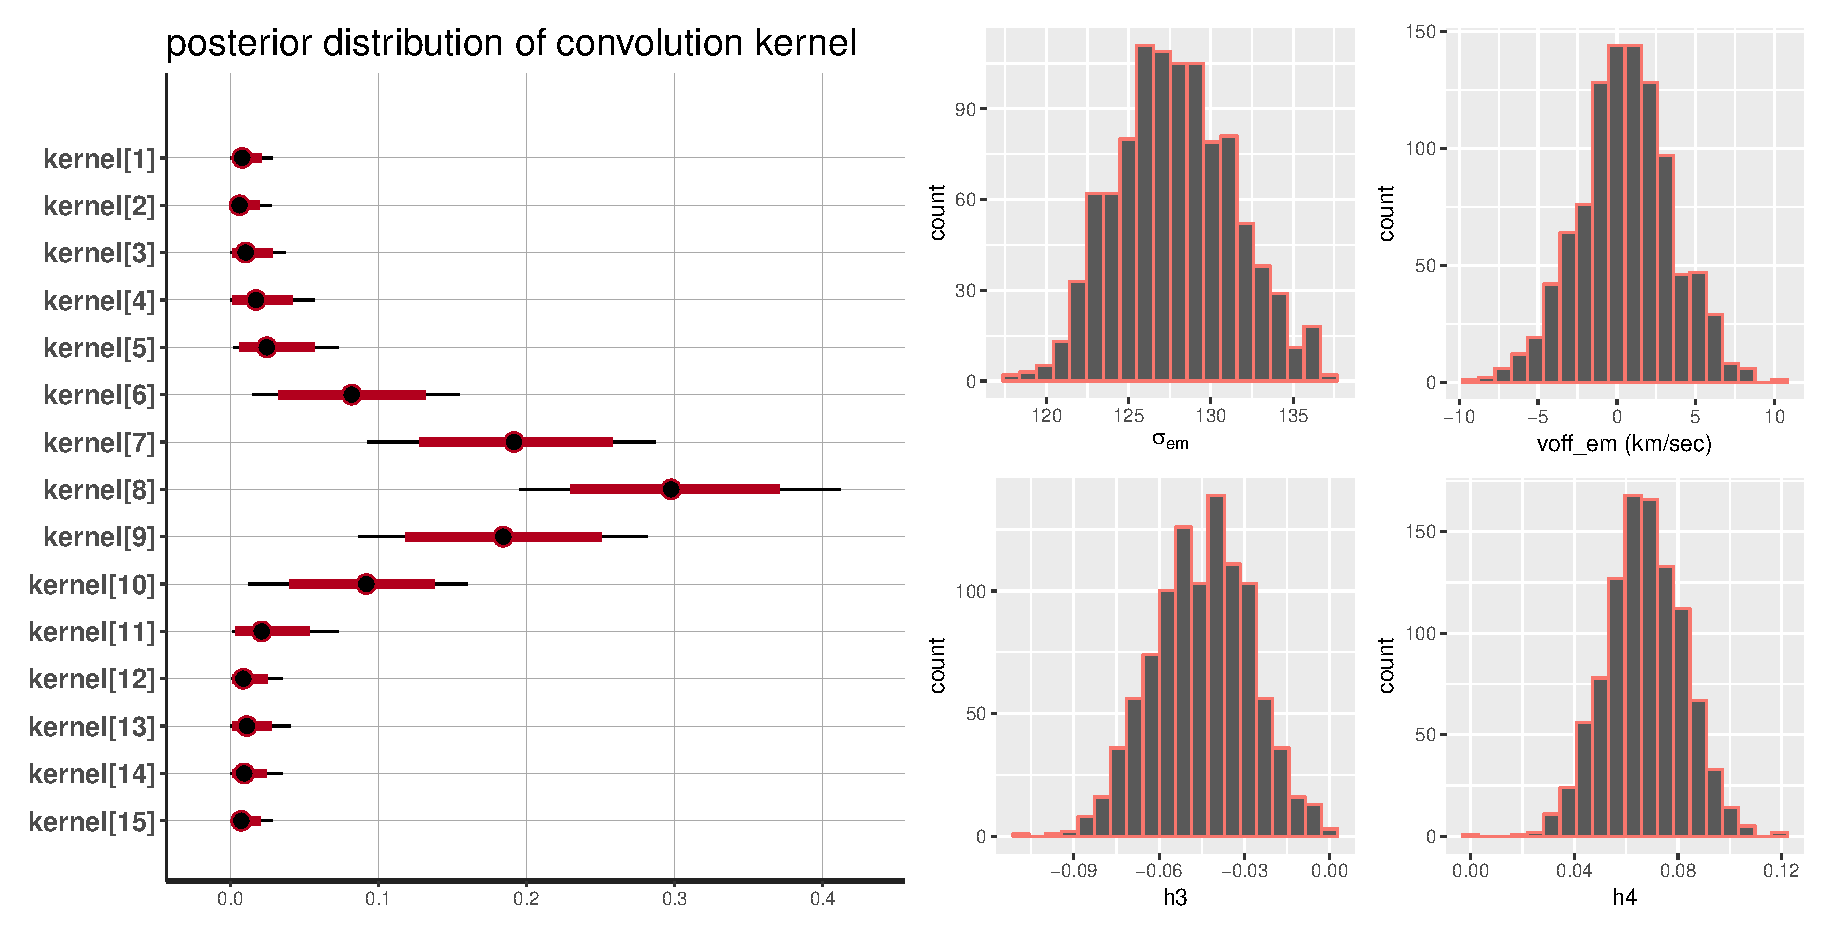
\includegraphics{losvd_1_256002.eps}}
\caption{Posterior distributions of the SSP matrix convolution kernel and parameters of the emission line LOSVD. Fit to the central fiber of mangaid 1-256002}
\label{fig:losvd_1_256002}
\end{figure*}

This model has to date only been run on a few sets of data. Execution time was about a factor of 30 longer than the code discussed in the text on the same data with the same set of SSP models, which is prohibitive for wholesale modeling on a desktop PC. From a pure technical standpoint Stan's performance on this model is quite good, with continued rapid convergence (based on number of iterations to reach stationary distributions).

I show a small set of results for a single model run on the central fiber of mangaid 1-256002. The posterior fit to the data is identical to figure \ref{fig:specfit} so I don't show it here. Posterior estimates of the kinematic parameters are shown in figure \ref{fig:losvd_1_256002}. The left pane shows the elements of the convolution kernel for the SSP model spectra. This is very close to symmetrical around the central element and close to a discretized Gaussian in profile. The parametric fits to the gas LOSVD on the right all appear to be well constrained. The velocity dispersion estimate is $\sigma_{em} = 127.8 \pm 3.5 (1 \sigma)$km/sec. That compares to the ML estimate for a single component gaussian for this data set of $127.6 \pm 2.2$, where the uncertainty was estimated from the inverse of the Hessian. This is excellent agreement; the slightly higher uncertainty estimate in the Bayesian fit probably results from marginalizing over everything else. Note finally that the coefficients of the higher order Gauss-Hermite moments are distributed well away from zero despite the strong priors, indicating a small asymmetry in the emission line profiles.

\begin{figure*}[ht]
\resizebox{\textwidth}{!}{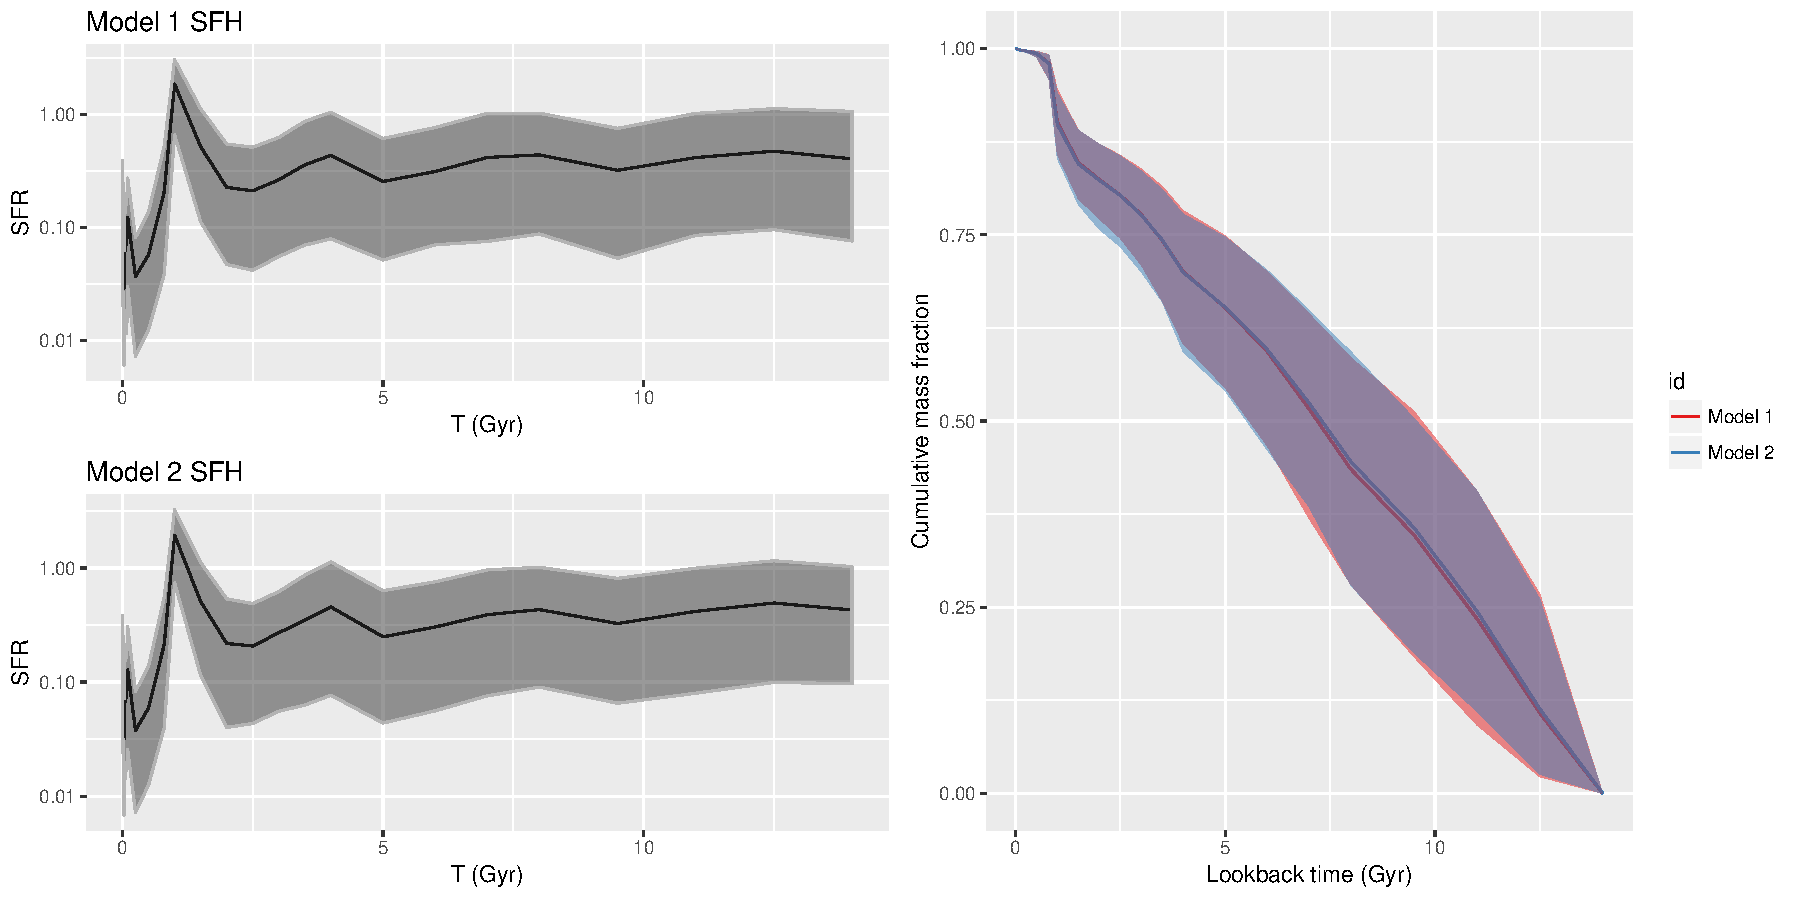
\includegraphics{sfhmgh_1_256002.pdf}}
\caption{Star formation and mass growth histories from posterior fits to the central fiber of mangaid 1-256002. Model 1 is the SFH model discussed in the text and listed in appendix \ref{sec:code}. Model 2 refers to the code in this section.}
\label{fig:sfhmgh_1_256002}
\end{figure*}

A slight surprise (figure \ref{fig:sfhmgh_1_256002}) is that star formation and mass growth histories are indistinguishable (some variation will be seen from one run to another of the same model unless the starting random number seed is fixed). Contrary to the expectation I expressed in section \ref{sec:bayes} marginalizing over kinematics had no effect at all on star formation history estimates. This is a welcome result since it suggests kinematics and star formation histories are separable problems, although it remains to be seen if this holds in systems with more complex kinematics.


\lstinputlisting{spm_ppvd.stan}

\bibliography{bayesspm}

%\begin{figure*}
%\centering
%\resizebox{\textwidth}{!}{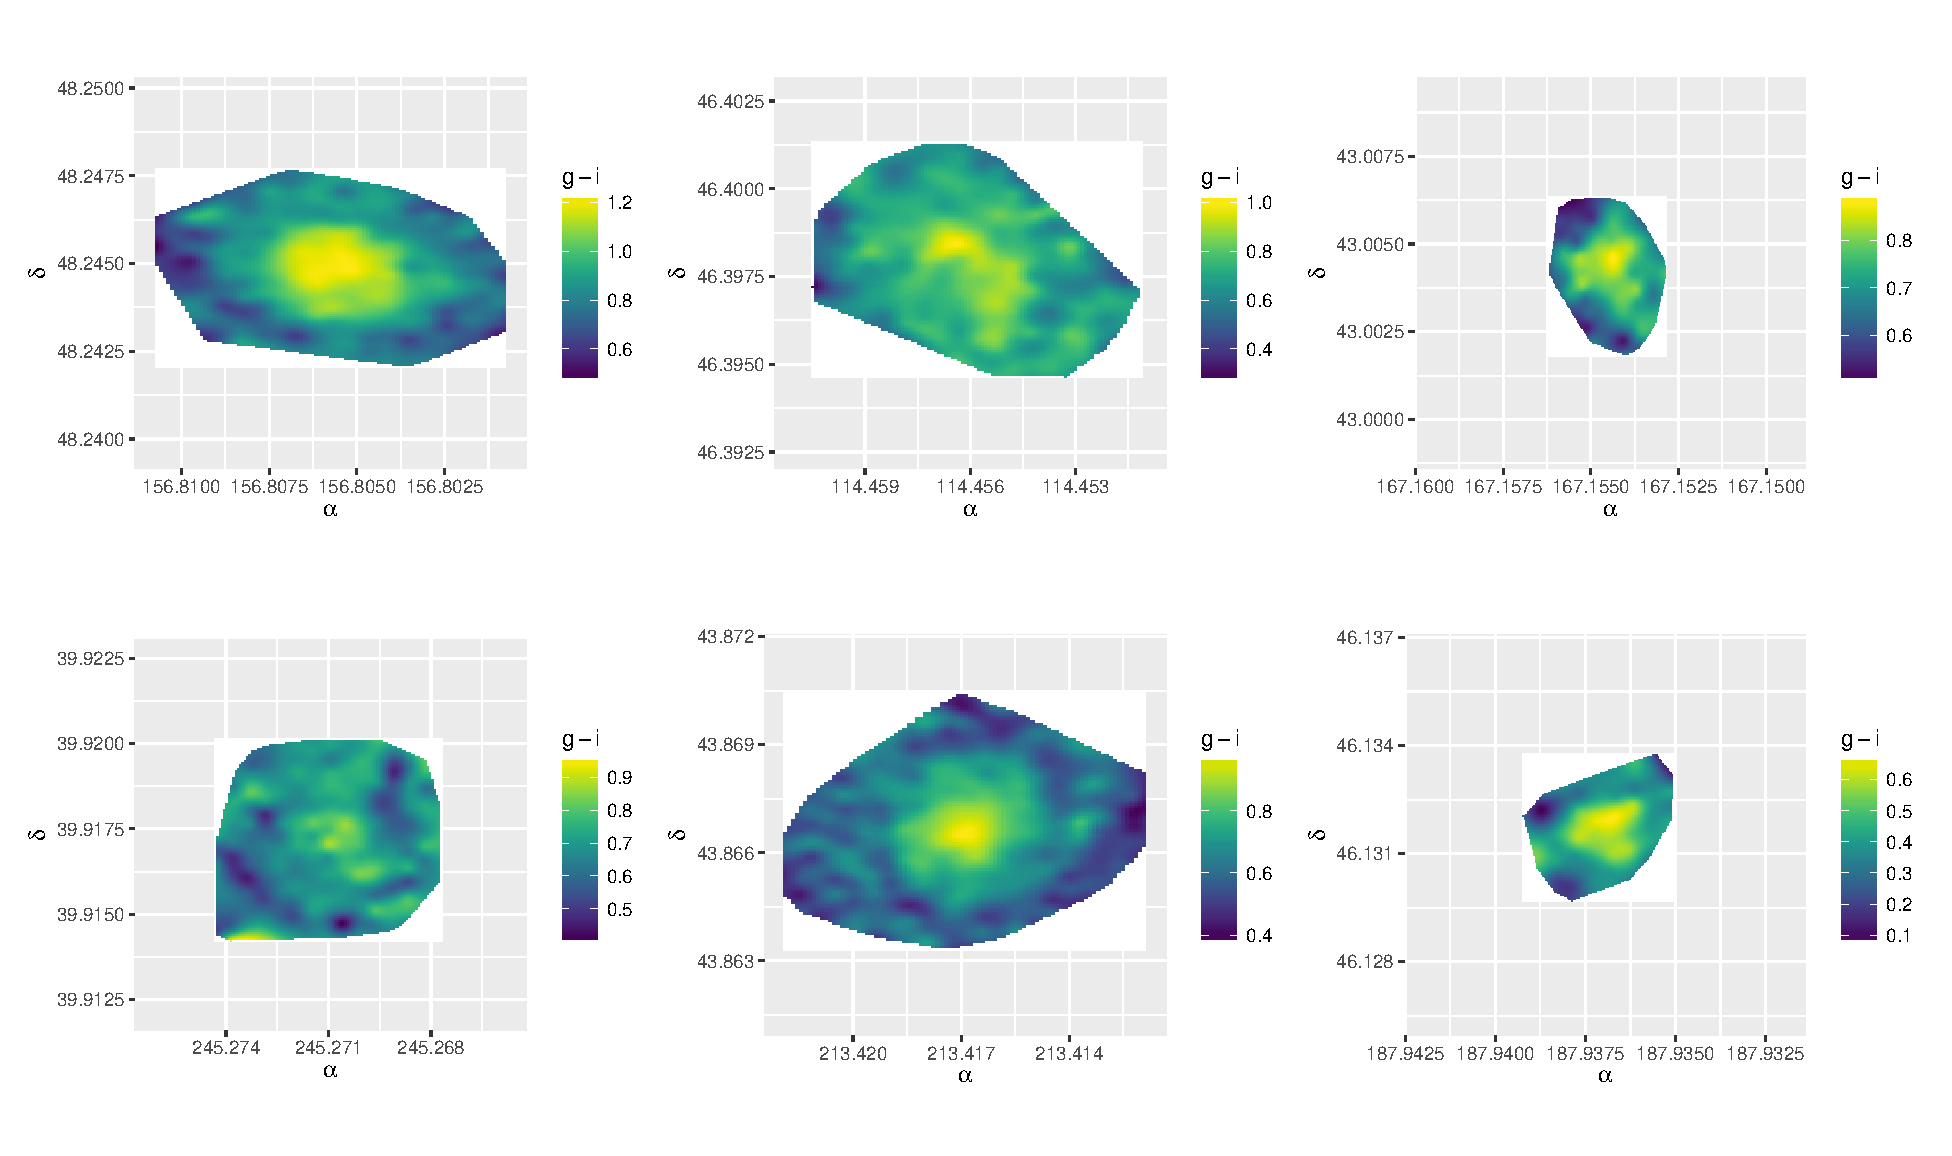
\includegraphics{g_imaps.eps}}
%\caption{Modeled g-i color. This is the estimated dereddened intrinsic color due to starlight only.}
%\label{fig:g_imaps}
%\end{figure*}

%\begin{figure*}
%\centering
%\resizebox{\textwidth}{!}{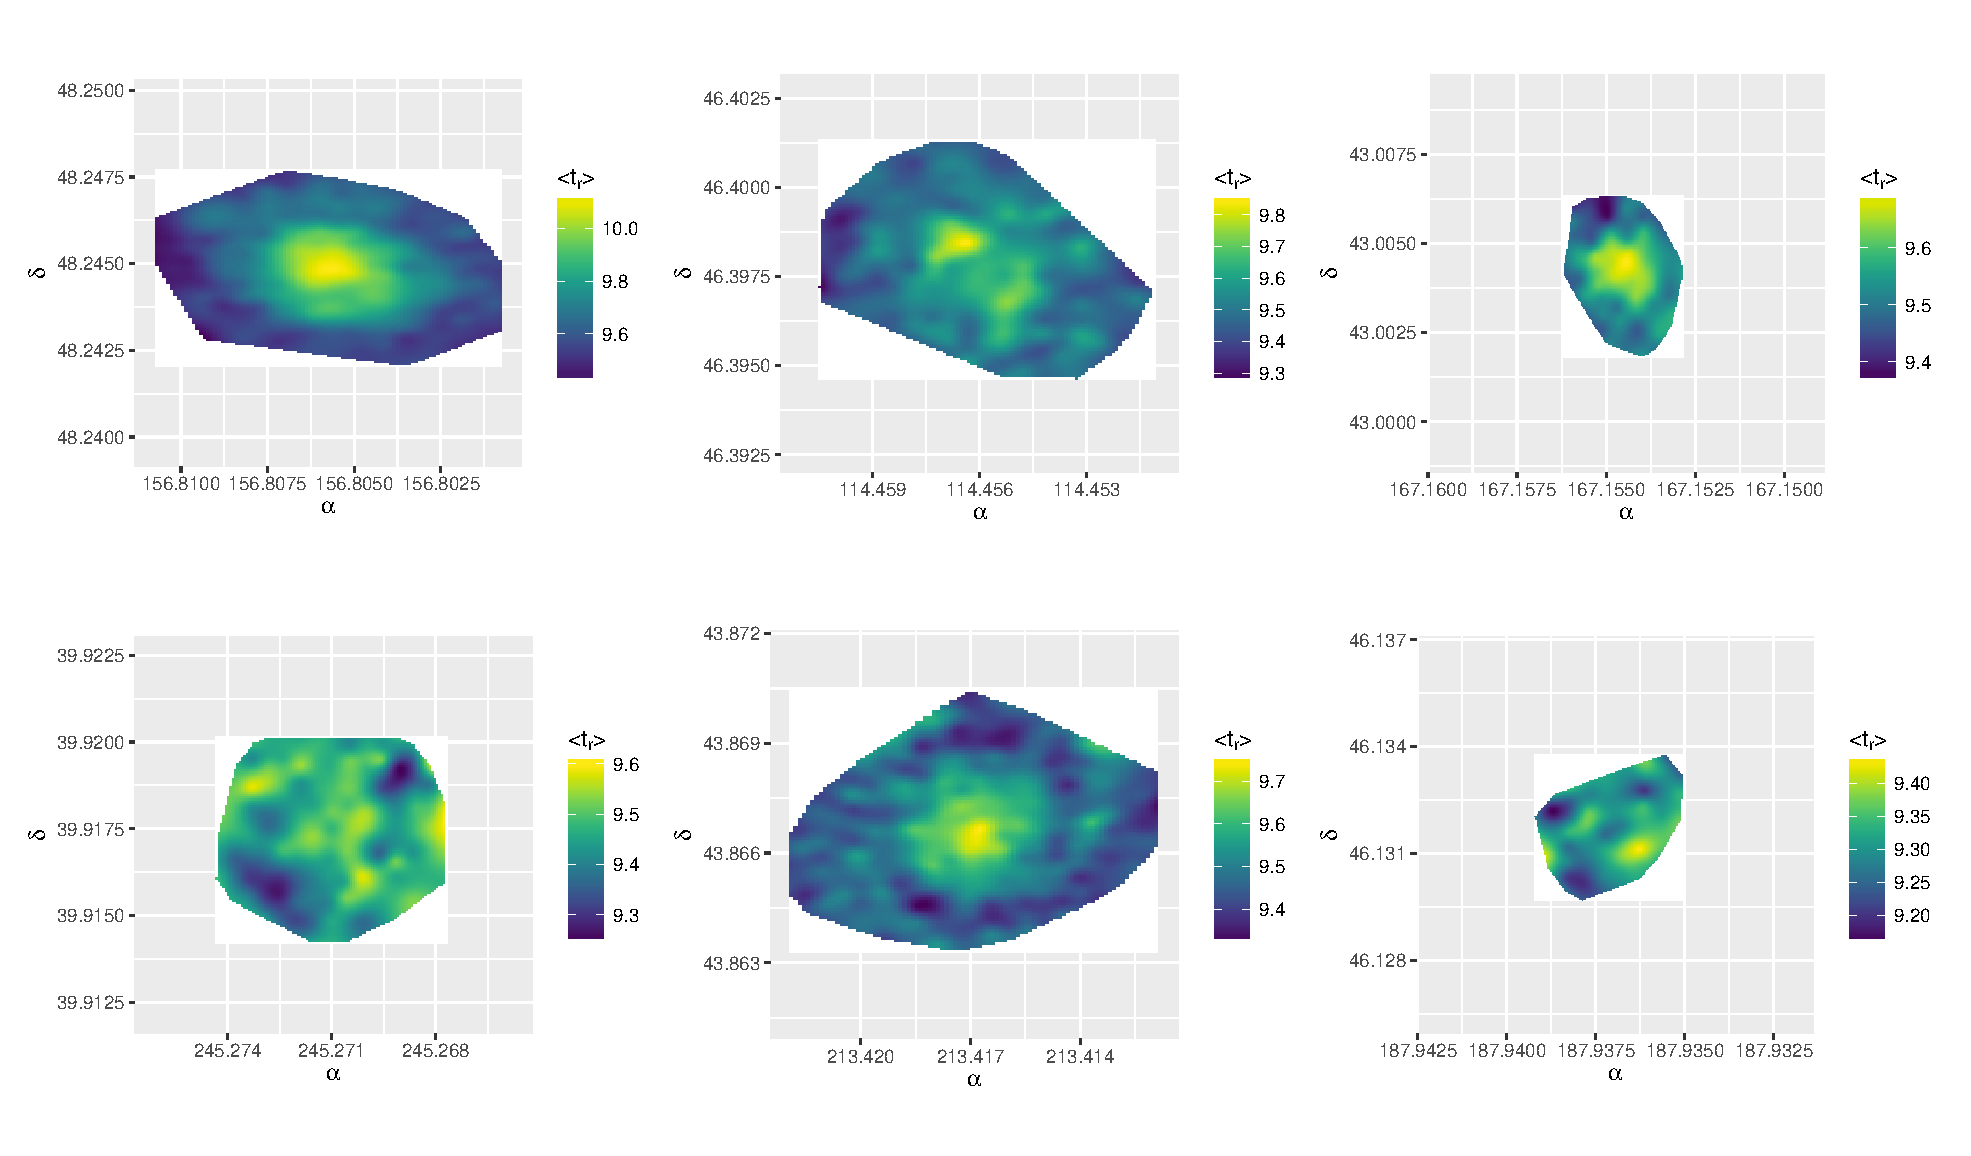
\includegraphics{tbar_lummaps.eps}}
%\caption{r band light weighted age ($yr$).}
%\label{fig:tbar_lummaps}
%\end{figure*}

\end{document}
